
\documentclass[hide notes,intlimits,unknownkeysallowed]{beamer}

\mode<presentation>
{
  \usetheme[footline]{UAFshade}
  \setbeamercovered{transparent}
}

% load packages
\usepackage{tikz}
\usetikzlibrary{shapes,arrows,shadows}
\usepackage{bm}
\usepackage[english]{babel}
\usepackage[latin1]{inputenc}
\usepackage[T1]{fontenc}
\usepackage{multimedia}
\usepackage[multidot]{grffile}

\usepackage{tikz}
\usetikzlibrary{shapes,arrows,shadows, calc}

%\usepackage{hyperref}

% Some useful commands (from ELB)
\newcommand{\bD}{\mathbf{D}}
\newcommand{\bbf}{\mathbf{f}}
\newcommand{\bF}{\mathbf{F}}
\newcommand{\bg}{\mathbf{g}}
\newcommand{\bn}{\mathbf{n}}
\newcommand{\bq}{\mathbf{q}}
\newcommand{\bT}{\mathbf{T}}
\newcommand{\bu}{\mathbf{u}}
\newcommand{\bU}{\mathbf{U}}
\newcommand{\bv}{\mathbf{v}}

%% commands to facilitate units and temperature
\newcommand{\unit}[1]{\ensuremath{\,\mathrm{#1}}}
\newcommand{\s}[1]{\ensuremath{\,\mathrm{#1}}}
\newcommand{\cels}[1]{\ensuremath{#1^{\circ}\,\mathrm{C}}}


\newcommand{\hbe}{\hat{\mathbf{e}}}
%\newcommand{\define}[1]{{\textbf{#1}}\marginpar{\psshadowbox[framearc=0.3,shadowsize=2pt]{\footnotesize #1}}}
\newcommand{\define}[1]{{\textbf{#1}}\marginpar{\fbox{\footnotesize #1}}}
\newcommand{\epsdot}{\dot{\varepsilon}}
\newcommand{\bsigma}{\mbox{\boldmath$\sigma$\unboldmath}}
\newcommand{\bepsdot}{\mbox{\boldmath$\epsdot$\unboldmath}}


% some parameters for customization
\def\shadowshift{3pt,-3pt}
\def\shadowradius{6pt}

\colorlet{innercolor}{black!60}
\colorlet{outercolor}{gray!05}

% this draws a shadow under a rectangle node
\newcommand\drawshadow[1]{
    \begin{pgfonlayer}{shadow}
        \shade[outercolor,inner color=innercolor,outer color=outercolor] ($(#1.south west)+(\shadowshift)+(\shadowradius/2,\shadowradius/2)$) circle (\shadowradius);
        \shade[outercolor,inner color=innercolor,outer color=outercolor] ($(#1.north west)+(\shadowshift)+(\shadowradius/2,-\shadowradius/2)$) circle (\shadowradius);
        \shade[outercolor,inner color=innercolor,outer color=outercolor] ($(#1.south east)+(\shadowshift)+(-\shadowradius/2,\shadowradius/2)$) circle (\shadowradius);
        \shade[outercolor,inner color=innercolor,outer color=outercolor] ($(#1.north east)+(\shadowshift)+(-\shadowradius/2,-\shadowradius/2)$) circle (\shadowradius);
        \shade[top color=innercolor,bottom color=outercolor] ($(#1.south west)+(\shadowshift)+(\shadowradius/2,-\shadowradius/2)$) rectangle ($(#1.south east)+(\shadowshift)+(-\shadowradius/2,\shadowradius/2)$);
        \shade[left color=innercolor,right color=outercolor] ($(#1.south east)+(\shadowshift)+(-\shadowradius/2,\shadowradius/2)$) rectangle ($(#1.north east)+(\shadowshift)+(\shadowradius/2,-\shadowradius/2)$);
        \shade[bottom color=innercolor,top color=outercolor] ($(#1.north west)+(\shadowshift)+(\shadowradius/2,-\shadowradius/2)$) rectangle ($(#1.north east)+(\shadowshift)+(-\shadowradius/2,\shadowradius/2)$);
        \shade[outercolor,right color=innercolor,left color=outercolor] ($(#1.south west)+(\shadowshift)+(-\shadowradius/2,\shadowradius/2)$) rectangle ($(#1.north west)+(\shadowshift)+(\shadowradius/2,-\shadowradius/2)$);
        \filldraw ($(#1.south west)+(\shadowshift)+(\shadowradius/2,\shadowradius/2)$) rectangle ($(#1.north east)+(\shadowshift)-(\shadowradius/2,\shadowradius/2)$);
    \end{pgfonlayer}
}

% create a shadow layer, so that we don't need to worry about overdrawing other things
\pgfdeclarelayer{shadow} 
\pgfsetlayers{shadow,main}

\newsavebox\mybox
\newlength\mylen

\newcommand\shadowimage[2][]{%
\setbox0=\hbox{\includegraphics[#1]{#2}}
\setlength\mylen{\wd0}
\ifnum\mylen<\ht0
\setlength\mylen{\ht0}
\fi
\divide \mylen by 120
\def\shadowshift{\mylen,-\mylen}
\def\shadowradius{\the\dimexpr\mylen+\mylen+\mylen\relax}
\begin{tikzpicture}
\node[anchor=south west,inner sep=0] (image) at (0,0) {\includegraphics[#1]{#2}};
\drawshadow{image}
\end{tikzpicture}}

\newcommand\shadowimagec[3][]{%
\setbox0=\hbox{\includegraphics<#1>[#2]{#3}}
\setlength\mylen{\wd0}
\ifnum\mylen<\ht0
\setlength\mylen{\ht0}
\fi
\divide \mylen by 120
\def\shadowshift{\mylen,-\mylen}
\def\shadowradius{\the\dimexpr\mylen+\mylen+\mylen\relax}
\begin{tikzpicture}
\node[anchor=south west,inner sep=0] (image) at (0,0) {\includegraphics<#1>[#2]{#3}};
\drawshadow{image}
\end{tikzpicture}}


\graphicspath{{figures/}}

\newenvironment{transbox}{%

\begin{tikzpicture}
\node[drop shadow,rounded corners,text width=\textwidth,fill=white, fill opacity=0.75,text opacity=1] \bgroup
}{
\egroup;\end{tikzpicture}}

\setbeamercolor{boxed}{fg=black,bg=uaf yellow}


% title page
\title[Glacier Dynamics] % (optional, use only with long paper titles)
{Why do glaciers flow?}
\subtitle{McCarthy Summer School, June 2024}

\author[Aschwanden] % (optional, use only with lots of authors)
{Andy Aschwanden}
% - Give the names in the same order as the appear in the paper.
% - Use the \inst{?} command only if the authors have different
%   affiliation.

\institute[GI] % (optional, but mostly needed)
{
  Geophysical Institute\\
  University of Alaska Fairbanks, USA
}
% - Use the \inst command only if there are several affiliations.
% - Keep it simple, no one is interested in your street address.

\titlegraphic{\shadowimage[width=.95\textwidth]{gris-nw-speed-exp-600m}}

\date{}
\subject{Glaciers}

\begin{document}

\AtBeginSection[]
{
  \begin{frame}<handout:0>
    \frametitle{Outline}
    \tableofcontents[sectionstyle=show/shaded,subsectionstyle=hide]
  \end{frame}
}


\setbeamertemplate{background canvas}
  {
     \tikz{\node[inner sep=0pt,opacity=1.0] {\includegraphics[width=\paperwidth]{uaf_beamer_shade_bg}};}
} 

% insert titlepage
\begin{frame}
  \titlepage
\end{frame}

\setbeamertemplate{background canvas}
{
%
} 

\setbeamertemplate{background canvas}
  {
     \tikz{\node[inner sep=0pt,opacity=0.75] {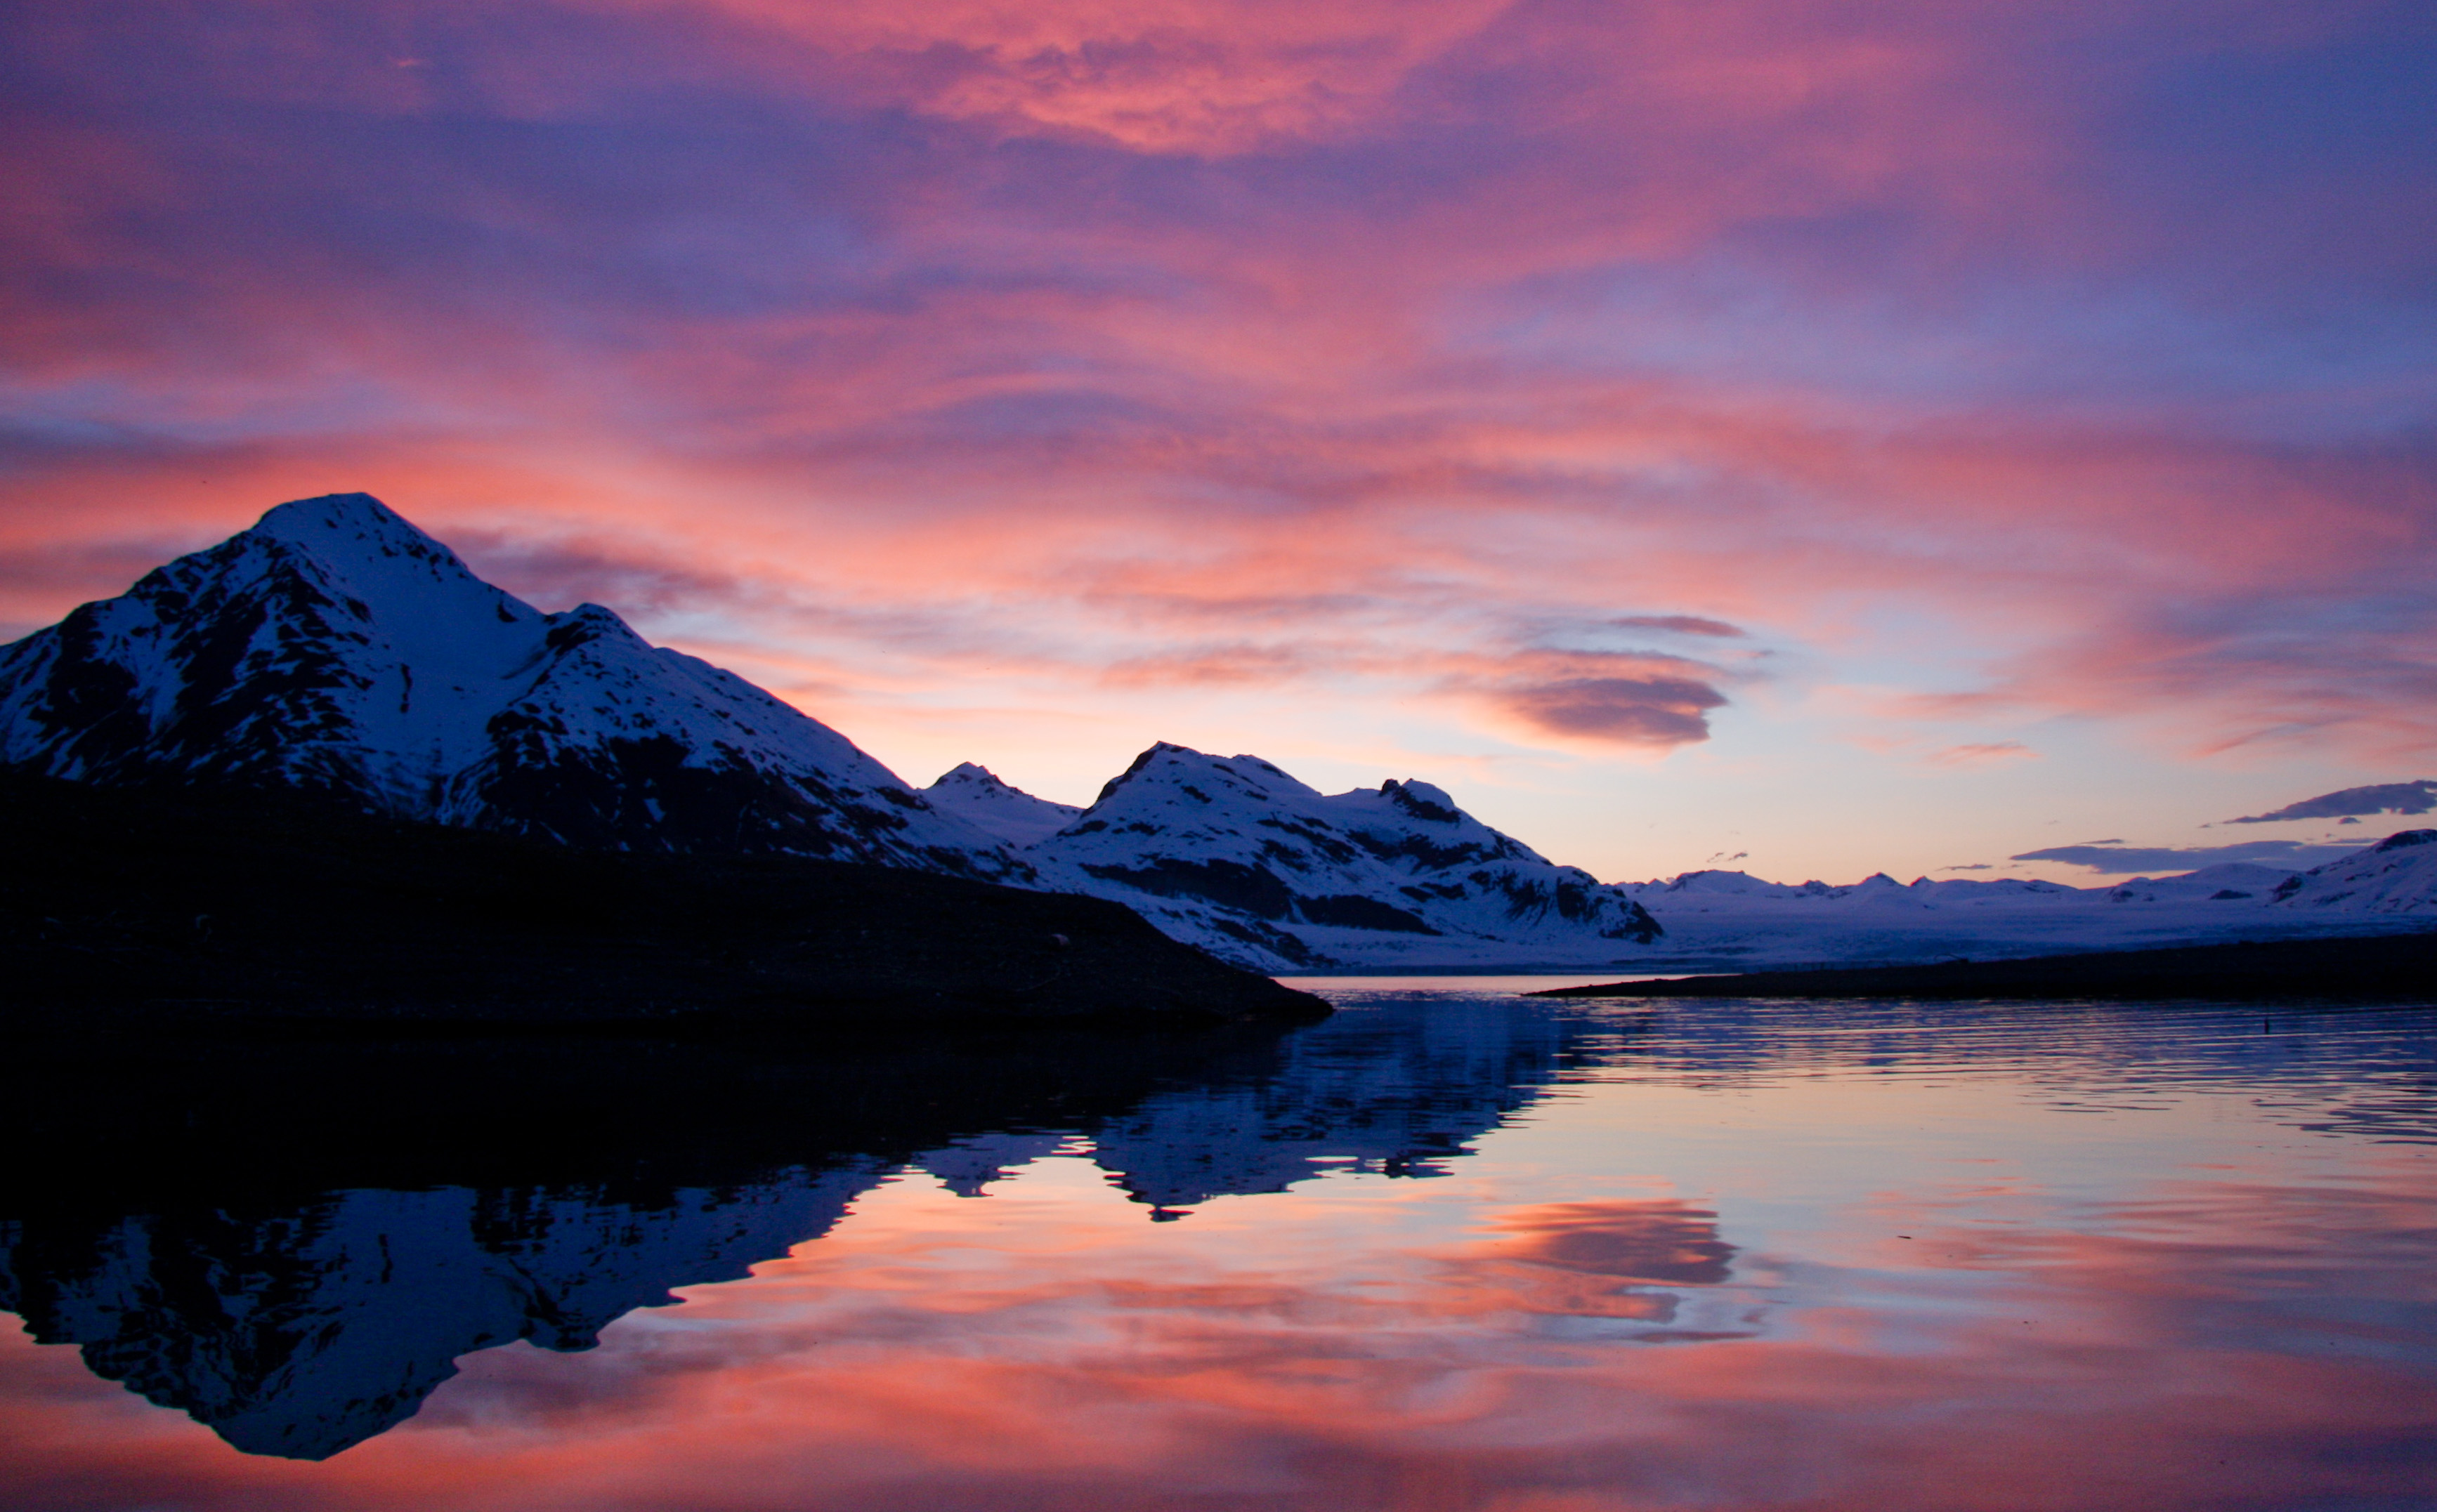
\includegraphics[height=
\paperheight,width=\paperwidth]{yakutat_sunset}};}
} 

\begin{frame}[plain] % not in the handout
  \begin{columns}
    \column[C]{7.5cm}
  \begin{transbox}
    \Large{``The most interesting fact about glaciers is that they flow''} \\[1.0em]
\emph{Garry Clark, J. Glaciol. (1987)}
  \end{transbox}
\end{columns}
\end{frame}



\setbeamertemplate{background canvas}
  {
     \tikz{\node[inner sep=0pt,opacity=.75] {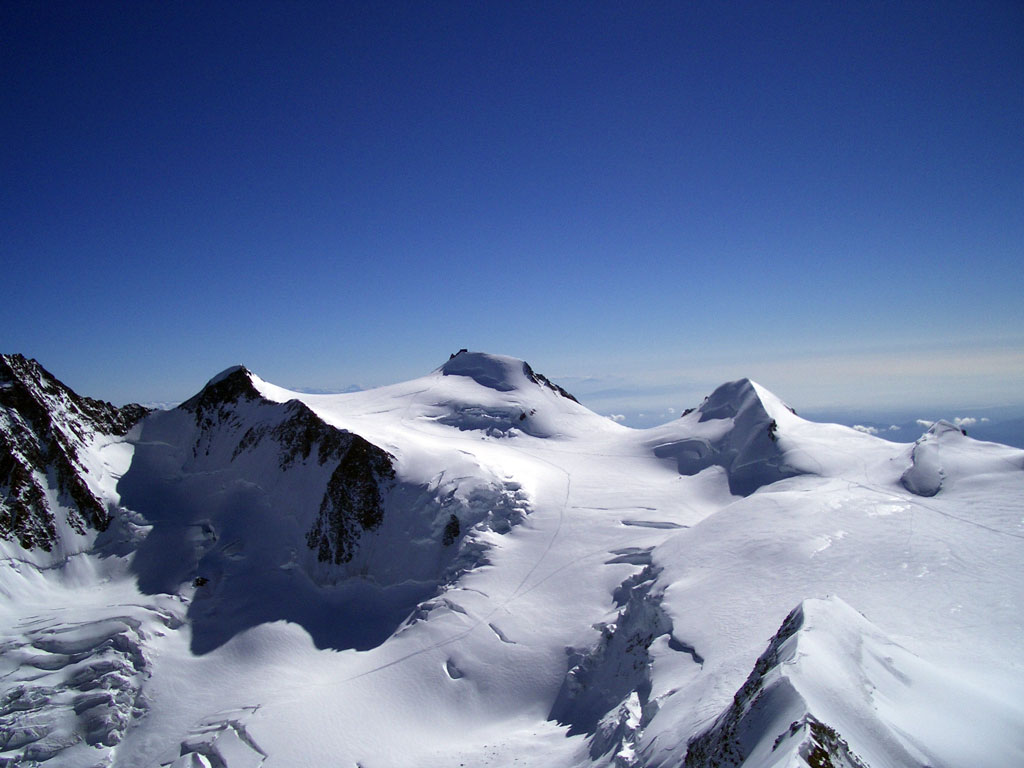
\includegraphics[height=
\paperheight,width=\paperwidth]{colle}};}
} 

\begin{frame}[plain]
  \begin{transbox}
    \begin{block}{What is a glacier?}
      \begin{itemize}[<+- | alert@+>] % some control parameters
      \item Artists, Tourists: beautiful landscape
      \item Geographers: element of landscape
      \item Geologists: soft rock, sediment
      \item Hydrologists: water reservoir
      \item Climatologists: subsystem of climate system, climate archive
      \item Physicists: thermomechanical non-Newtonian fluid
      \item Mathematicians: free boundary problem in fluid dynamics
      \item Electrical engineers: one sided accessible dielectric
      \item Glaciologists: part of the cryosphere
      \end{itemize} 
    \end{block}
  \end{transbox}
  \note[item]{Well, before we start talking about ice sheets, we need to ask the question: ``What is an ice sheet''?}
  \note[item]{Depending on who you ask, you may get quite different answers.}
\end{frame}

\setbeamertemplate{background canvas}
{
%
} 

\begin{frame}
  \frametitle{What is a glacier?}
  \centering{
    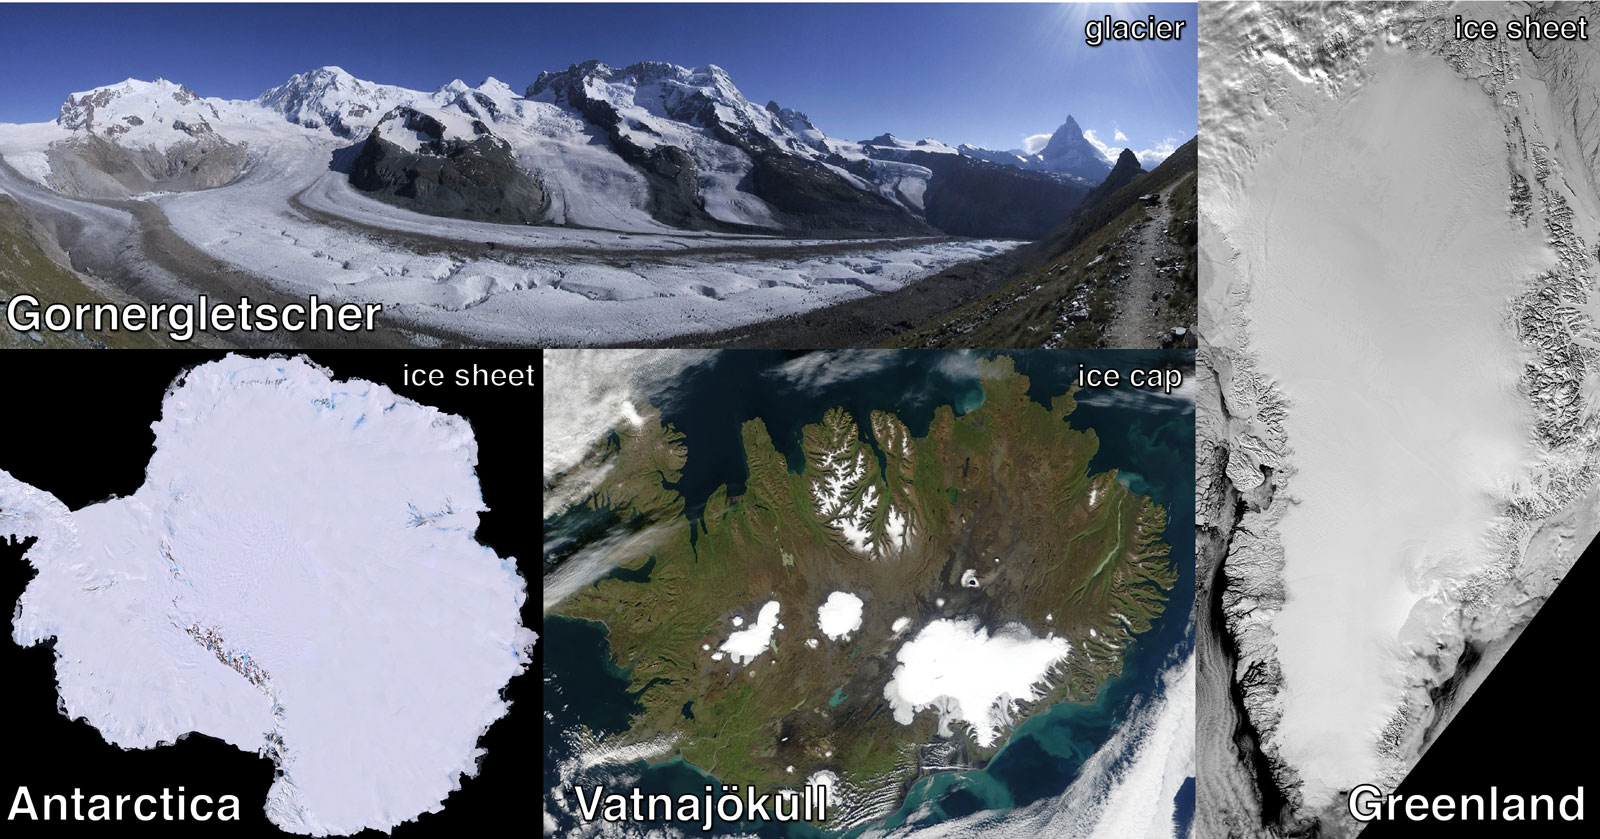
\includegraphics[width=.85\textwidth]{landice}
  }
  \begin{itemize}
  \item Glaciers flow slowly under their own weight
  \end{itemize}
  \note[itemize]{
    \item glaciers are the landice part of the cryosphere
}
\end{frame}


\begin{frame}
  \frametitle{Glacier flow vary over orders of magnitude}
  \begin{figure}
    \scriptsize{speeds by Evan Burgess (Wrangell) and Roman Motyka (Jakobshavn)}
    \includegraphics[width=.95\textwidth]{speeds-scale}
  \end{figure}
  \begin{itemize}
    \item observed speeds range from 20\,m\,a$^{-1}$ for a valley glacier to 15\,km\,a$^{-1}$ (``fast flow'')
  \end{itemize}
  \note[itemize]{
}
\end{frame}

\begin{frame}
  \frametitle{How does a glacier move?}
  \centering{
    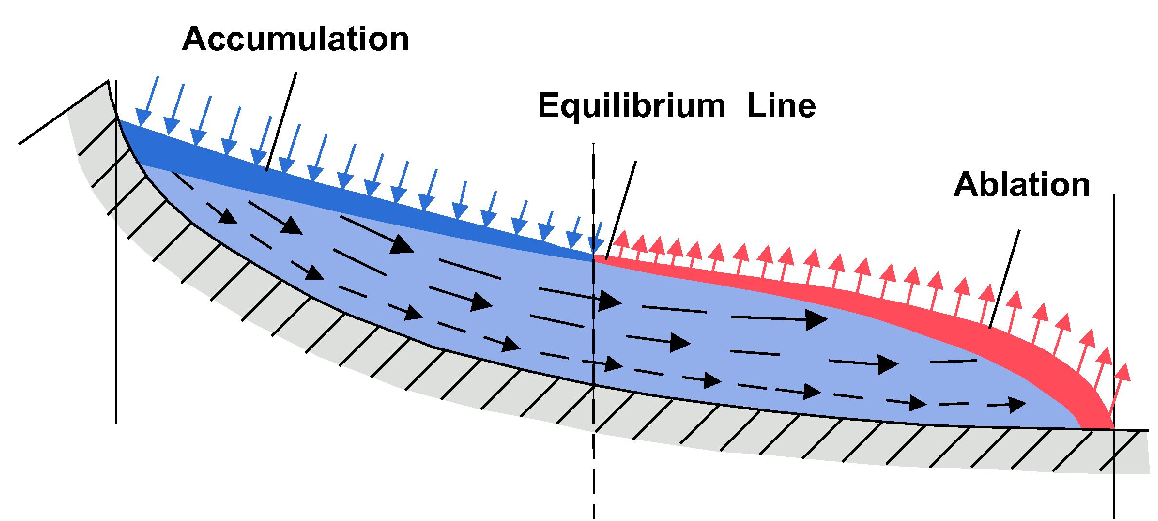
\includegraphics[width=.65\textwidth]{flow_acc_abl}
  }
  \begin{block}{In a nut shell:}
    \begin{itemize}
    \item Well-described by continuum mechanics (Martin's lecture)
    \item The ice can deform as a \alert{viscous} fluid
    \item The ice can slide over its substrate or the substrate deforms
    \end{itemize}
  \end{block}
\end{frame}

\begin{frame}{About viscosity $\eta$}
    \begin{columns}
      \column[C]{6cm}
      \begin{figure}
        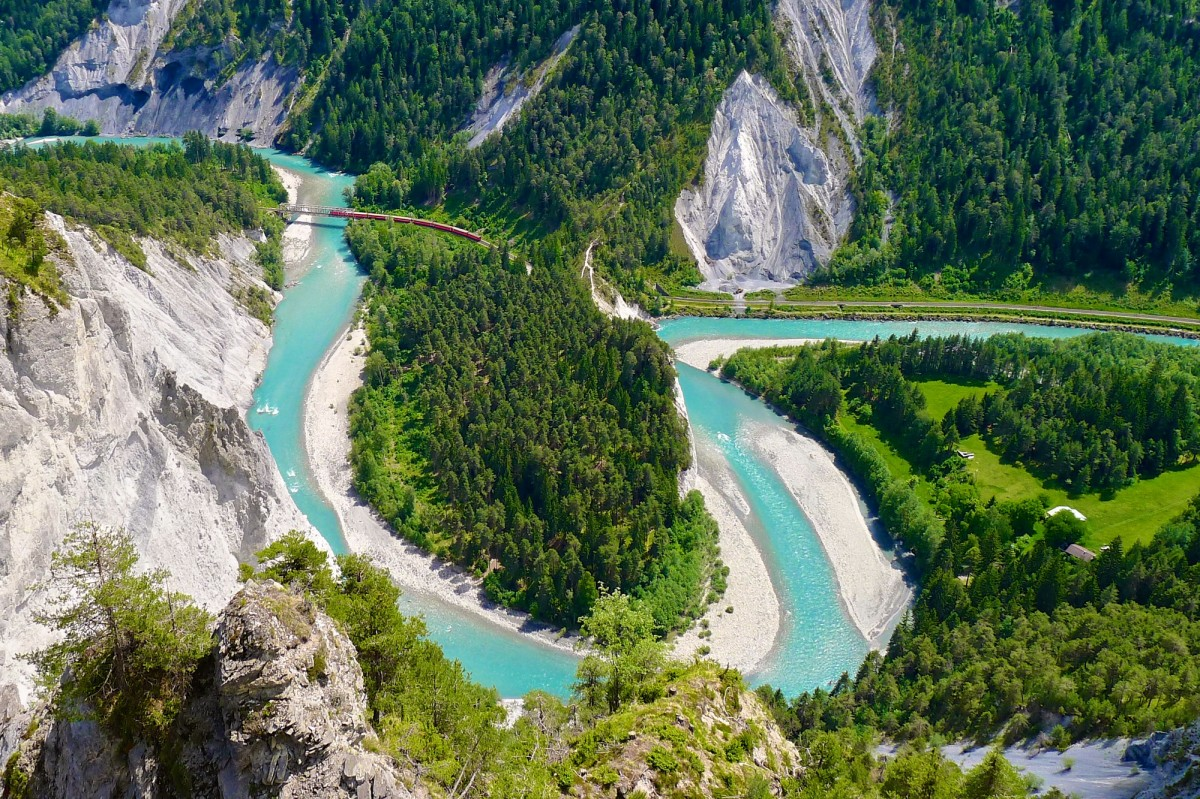
\includegraphics[height=3cm]{rhine_river}
      \end{figure}
      \column[C]{6cm}
      \begin{figure}
        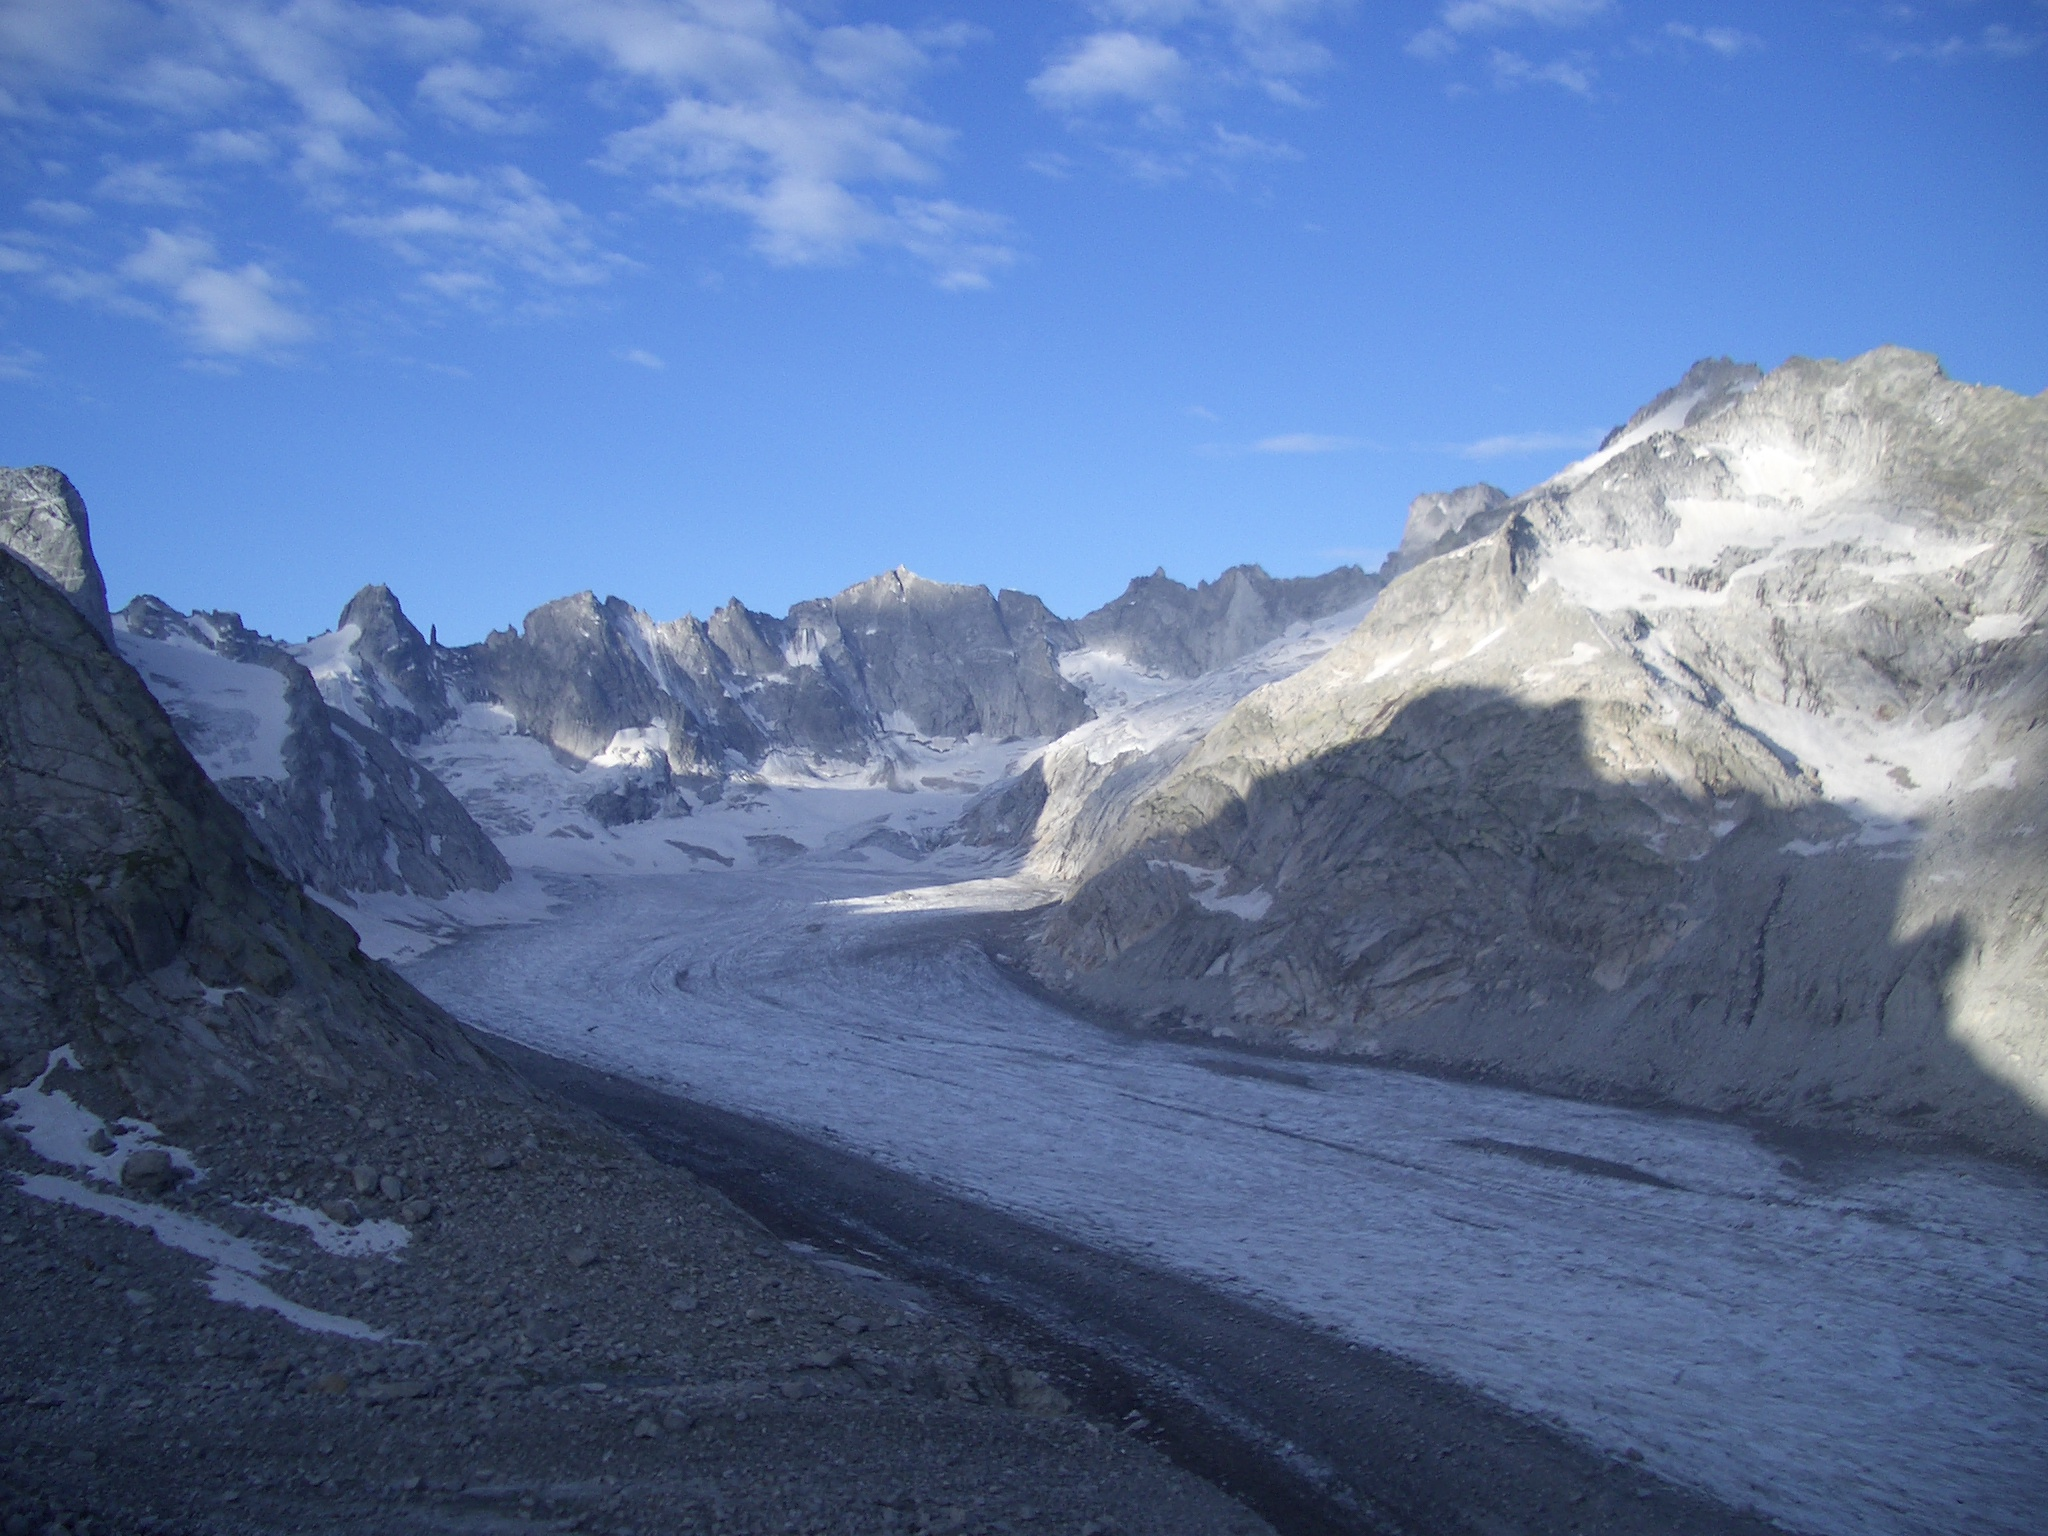
\includegraphics[height=3cm]{forno}
      \end{figure}
  \end{columns}
    \begin{columns}
      \column[C]{6cm}
      \begin{itemize}
        \item Newtonian fluid
        \item viscosity is constant ($10^{-3}$Pa\,s)
      \end{itemize}
      \column[C]{6cm}
      \begin{itemize}
      \item non-Newtonian fluid
        \item viscosity depends on temperature, water content, impurities, and on \alert{stress state}
      \end{itemize}
  \end{columns}
\end{frame}

\begin{frame}{Viscosity vs Glaciology}
  \begin{block}{Engineering and computational fluid dynamics (CFD)}
    Deformation causes stresses
  \begin{equation}
  \bm{\sigma}^{(d)} = 2 \eta \bm{\epsdot}
  \end{equation}
  \end{block}
  \begin{block}{Glaciology}
    Stresses cause deformation
  \begin{equation}
  \bm{\epsdot} = A \bm{\tau}^{n-1}  \bm{\sigma}^{(d)}
  \end{equation}
  \end{block}
  \alert{$\Rightarrow$} This can be confusing to ``outsiders''. The viscosity is given by
  \begin{equation}
    \eta = \frac{1}{2 A(T,\omega,\ldots) \sigma_{\mathrm{e}}^{n-1}}
  \end{equation}
\end{frame}

\begin{frame}{From Navier Stokes to Stokes}
  \begin{block}{From the (incompressible) Navier Stokes Equations}
    \begin{eqnarray}
      \nabla \cdot \bm{v} & = & 0 \\
    \rho \underbrace{\frac{\textrm{d} {\bm{v}}}{\textrm{d} t}}_{acceleration} & = & \underbrace{-\nabla p}_{pressure} +  \underbrace{\nabla \cdot \bm{\sigma}^{(d)}}_{viscous}  + \underbrace{\rho\bm{g}}_{gravity} + \underbrace{\rho\bm{f}}_{Coriolis}
  \end{eqnarray}
  \end{block}
  \begin{block}{to the (incompressible) Stokes Equation}
    \begin{eqnarray}
      \nabla \cdot \bm{v} & = & 0 \\
      \underbrace{\nabla \cdot \bm{\tau}}_{viscous} & = & - \underbrace{\rho\bm{g}}_{gravity}
    \end{eqnarray}
  \end{block}
\end{frame}

\begin{frame}{Scale Analysis}
  \begin{block}{Typical values}
    \begin{tabular}{lccc}
      & & glacier & ice sheet \\[.25em]
  \hline
  horizontal extent & L & 10\,km & 1,000\,km \\[.25em]
  \hline
  horizontal velocity & U & 10 \,m\,yr$^{-1}$ & 100\,m\,yr$^{-1}$ \\[.25em]
  \hline
  viscosity & $\eta$ & $10^{12}$\,Pa\,s & $10^{12}$\,Pa\,s \\[.25em]
  \hline
  gravity & G & \multicolumn{2}{c}{10\,m\,s$^{-1}$}\\[.25em]
  \hline
  pressure & P & \multicolumn{2}{c}{no natural scale} \\[.25em]
  \hline
\end{tabular}        
  \end{block}
  \begin{block}{Dimensionless numbers}\vspace{0.5em}
\begin{tabular}{lccccc}
\hline
Froude number & Fr & $\frac{\text{acceleration}}{\text{gravitational force}}$ & $\frac{U}{\sqrt{GL}}$ \\[.25em]
\hline
Rossby number & Ro & $\frac{\text{acceleration}}{\text{Coriolis force}}$ & $\frac{U}{2 \Omega L}$   \\[.25em]
\hline
Reynolds number & Re & $\frac{\text{acceleration}}{\text{viscous force}}$ & $\frac{\rho U L}{\eta}$ \\[.25em]
\hline
\end{tabular}        
  \end{block}
\end{frame}

\begin{frame}{Scaled Navier Stokes Equation}
  \begin{eqnarray}
    \nabla \cdot \bm{v}^* & = & 0 \\
    \frac{\textrm{d} {\bm{v}^*}}{\textrm{d} t^*} & = & -\frac{1}{Re}\nabla p^* +  \frac{1}{Re}\nabla \cdot \bm{\sigma}^{(d)^*}  + \frac{1}{Fr}\bm{g}^* + \frac{1}{Ro}\bm{f}^*
  \end{eqnarray}
  \begin{block}{Note}
    Greve and Blatter scale the pressure gradient by the overburden pressure $\rho g H$ instead of the viscous stress.
  \end{block}
\end{frame}

\begin{frame}{Gravity Driven Thin Film Flow}
  \alert{Note}: Similar to ``Parallel Sided Slab'' in Script but for any fluid with viscosity $\eta$.
  \begin{figure}
    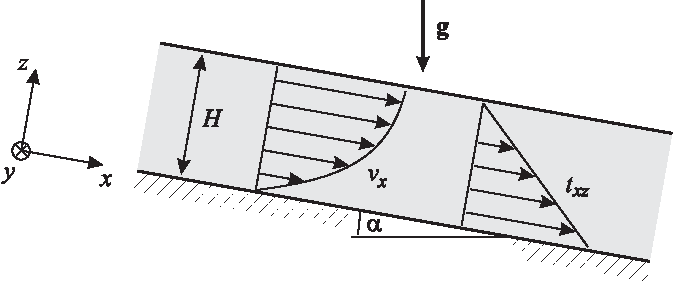
\includegraphics[width=7.5cm]{fig_3_11}
  \end{figure}
  \vspace{-1em}
  \begin{block}{Assumptions}
    \begin{itemize}
    \item[I] steady-state $\Rightarrow \mathrm{d} / \mathrm{d} t = 0$
    \item[II] uniform in x- and y-direction $\Rightarrow \partial / \partial x = \partial / \partial y = 0$
    \item[III] stress free surface $\Rightarrow \mathbf{T}\cdot \bn \vert_{z=H} = 0$
    \item[IV] no-slip at the base $\bv \vert_{z=b} = 0$
    \item[V] impenetrable basal plane 
%    \item[V] plane strain $\epsdot_{yx} = \epsdot_{yy} = \epsdot_{yz} = 0$
    \end{itemize}
  \end{block}
\end{frame}

\begin{frame}{Gravity Driven Thin Film Flow}
\begin{equation*}
    \begin{array}{ccl}
      v_x (z) &  = & \frac{\rho g}{\eta} \sin{\alpha}\left(Hz - \frac{z^2}{2}\right) \\[1em]
      p(z) & = & \rho g \left(H - z\right)\cos{\alpha}
    \end{array}
  \end{equation*}
\begin{block}{Noteworthy}
\begin{itemize}
\item this is an \alert{exact} solution of the incompressible Navier Stokes Equations.
\item horizontal velocity profile is \alert{parabolic}
\item pressure is \alert{hydrostatic}
\end{itemize}
\end{block}
\end{frame}

\begin{frame}{Flow of a Glacier in a Semi-Circular Valley}
  \vspace{-1em}
  \begin{figure}
    \centering
    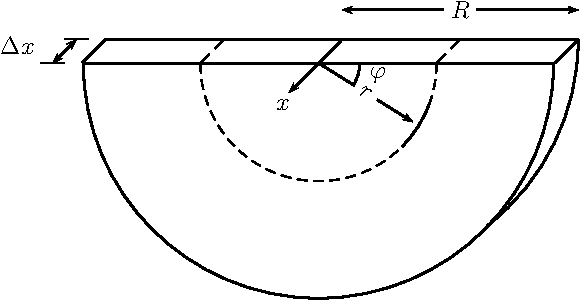
\includegraphics[width=0.4\textwidth]{fig_channel}
    \label{fig:valley-glacier-coord}
  \end{figure}
  \begin{block}{Assumptions}
    \begin{itemize}
    \item uniform in x- and $\varphi$-direction, steady-state $\Rightarrow \partial / \partial x = \partial / \partial \varphi = \partial / \partial t = 0$
    \item body force has to be balanced by tractions acting on the circumference in distance $r$ from the center
      \begin{equation*}
        \sigma_{rx} \pi r \Delta x = - \rho\,g\,\frac{\pi r^2}{2} \Delta x \sin \alpha
      \end{equation*}
\end{itemize}
  \end{block}
  \note[item]{Valley glacier: drag of the side walls}
\end{frame}

\begin{frame}{Flow of a Glacier in a Semi-Circular Valley}
 An analytical solution for the flow through a cylindrical channel can be obtained.
\begin{equation*}
v_x (r) = v_x (0) - \frac{2A}{n+1}\,\left( \frac{1}{2}\rho\,g\,\sin\alpha\right)^{n} r^{n+1}
\end{equation*}
\begin{block}{Noteworthy}
\begin{equation*}
v_{x, \text{channel}} = \left(\frac{1}{2}\right)^{n} v_{x, \text{slab}}
\end{equation*}
\begin{itemize}
\item here, the radius $R$ plays the role of the ice thickness $H$
\item center line velocity is \alert{eight} times slower than in an
  ice sheet of the same thickness (side wall drag)
\end{itemize}
\end{block}
\end{frame}


\begin{frame}
  \frametitle{Longitudinal Profile of a Valley Glacier}
  \begin{figure}
    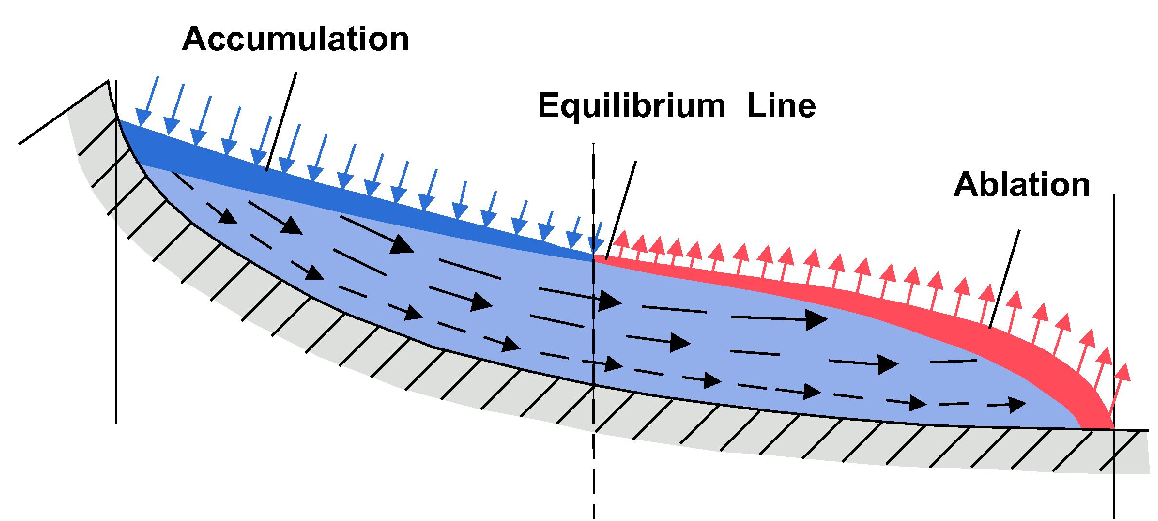
\includegraphics[width=\textwidth]{flow_acc_abl}
  \end{figure}
\end{frame}

\begin{frame}
  \frametitle{Evolution of the Glacier Surface}
  \begin{figure}
    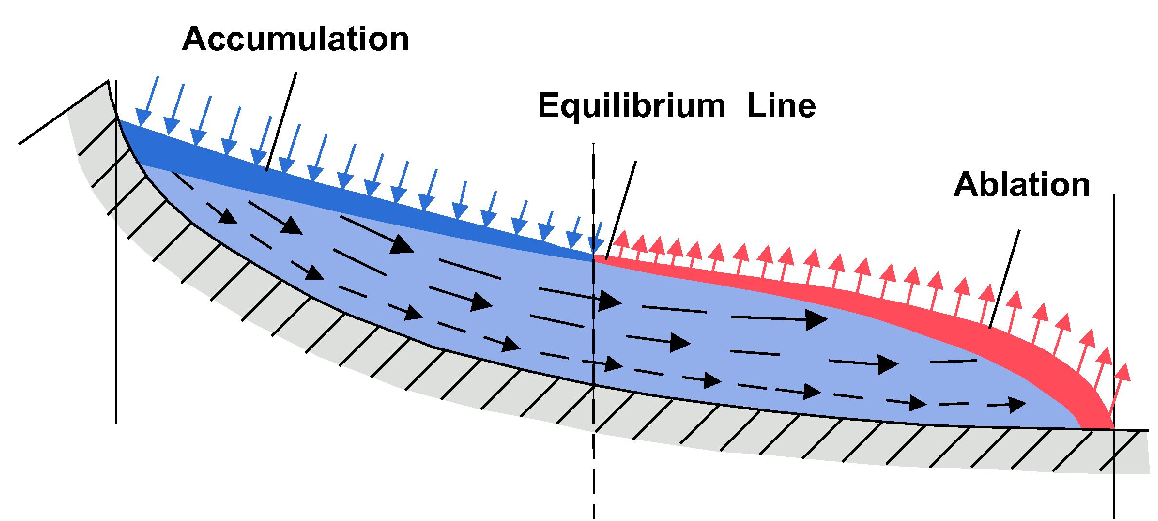
\includegraphics[width=.75\textwidth]{flow_acc_abl}
  \end{figure}
  Derivation on p. 12--14. Assuming $\partial b / \partial t = 0$ and no basal melt:
  \begin{equation*}
    \frac{\partial h}{\partial t} = \underbrace{-\nabla \cdot \mathbf{Q}}_{\text{dynamic changes}} \quad \underbrace{+B_{\text{clim}}}_{\text{climatic changes}}
  \end{equation*}
\end{frame}


\setbeamertemplate{background canvas}
{
%
} 



\begin{frame}
  \frametitle{Water plays an important role}
  \begin{figure}
    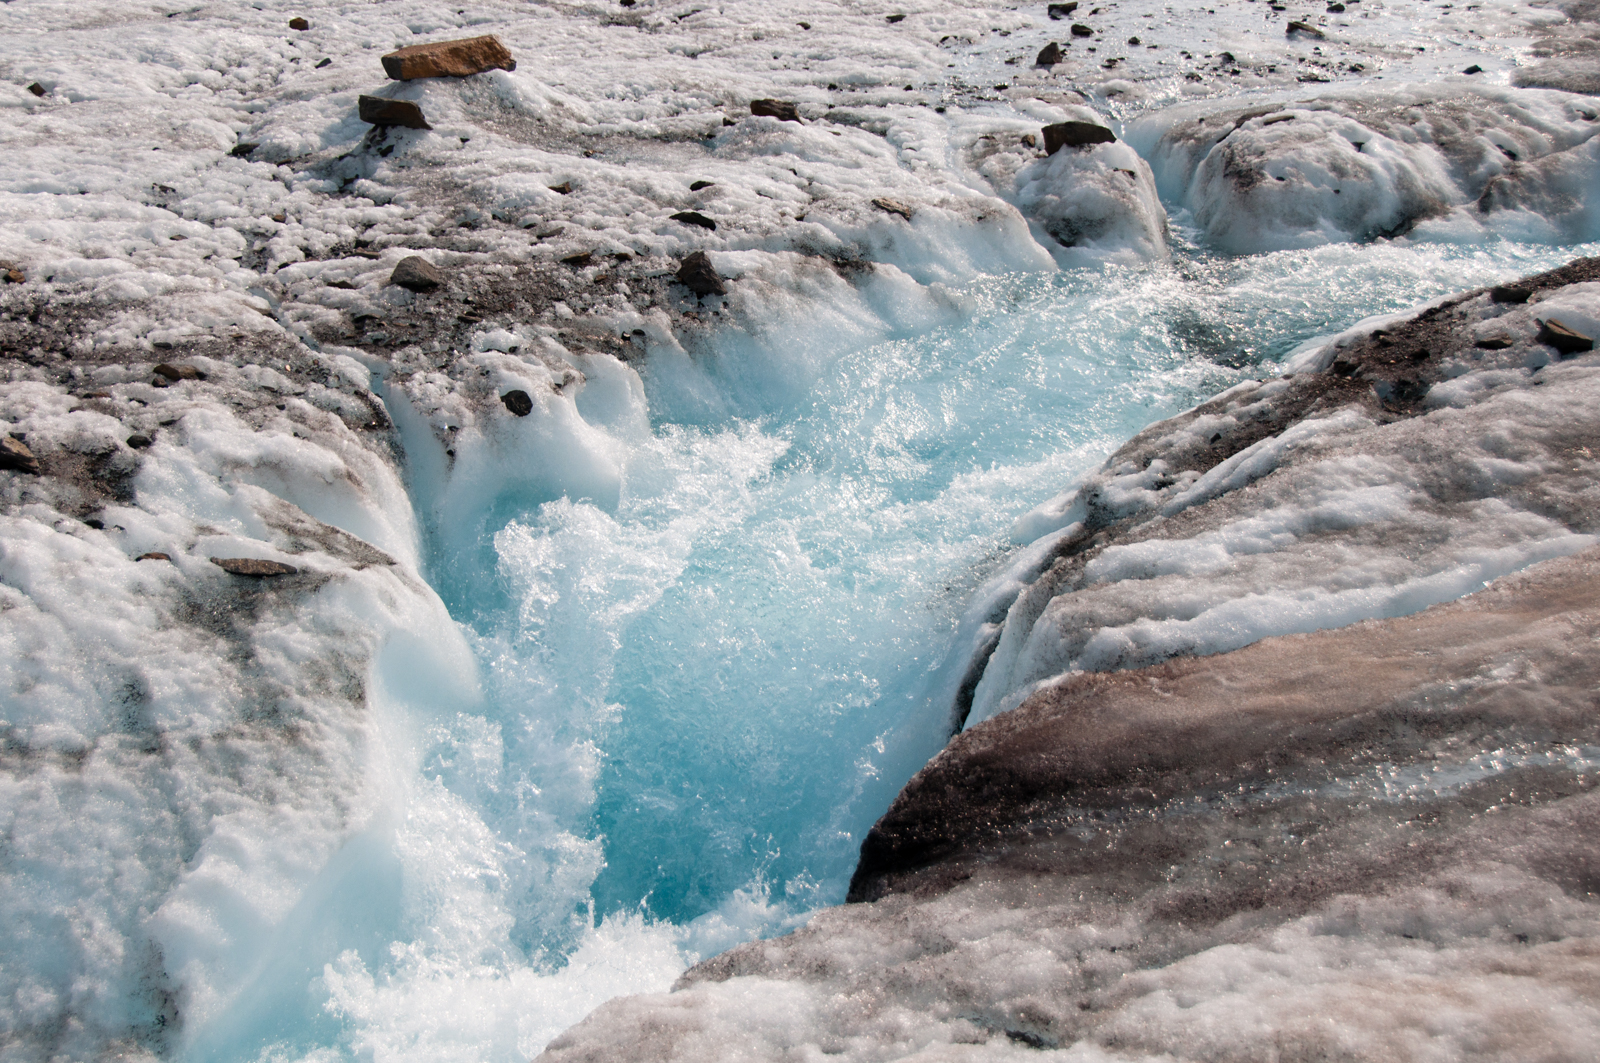
\includegraphics[height=5cm]{black-rapids-1} \vspace{0.25em}
    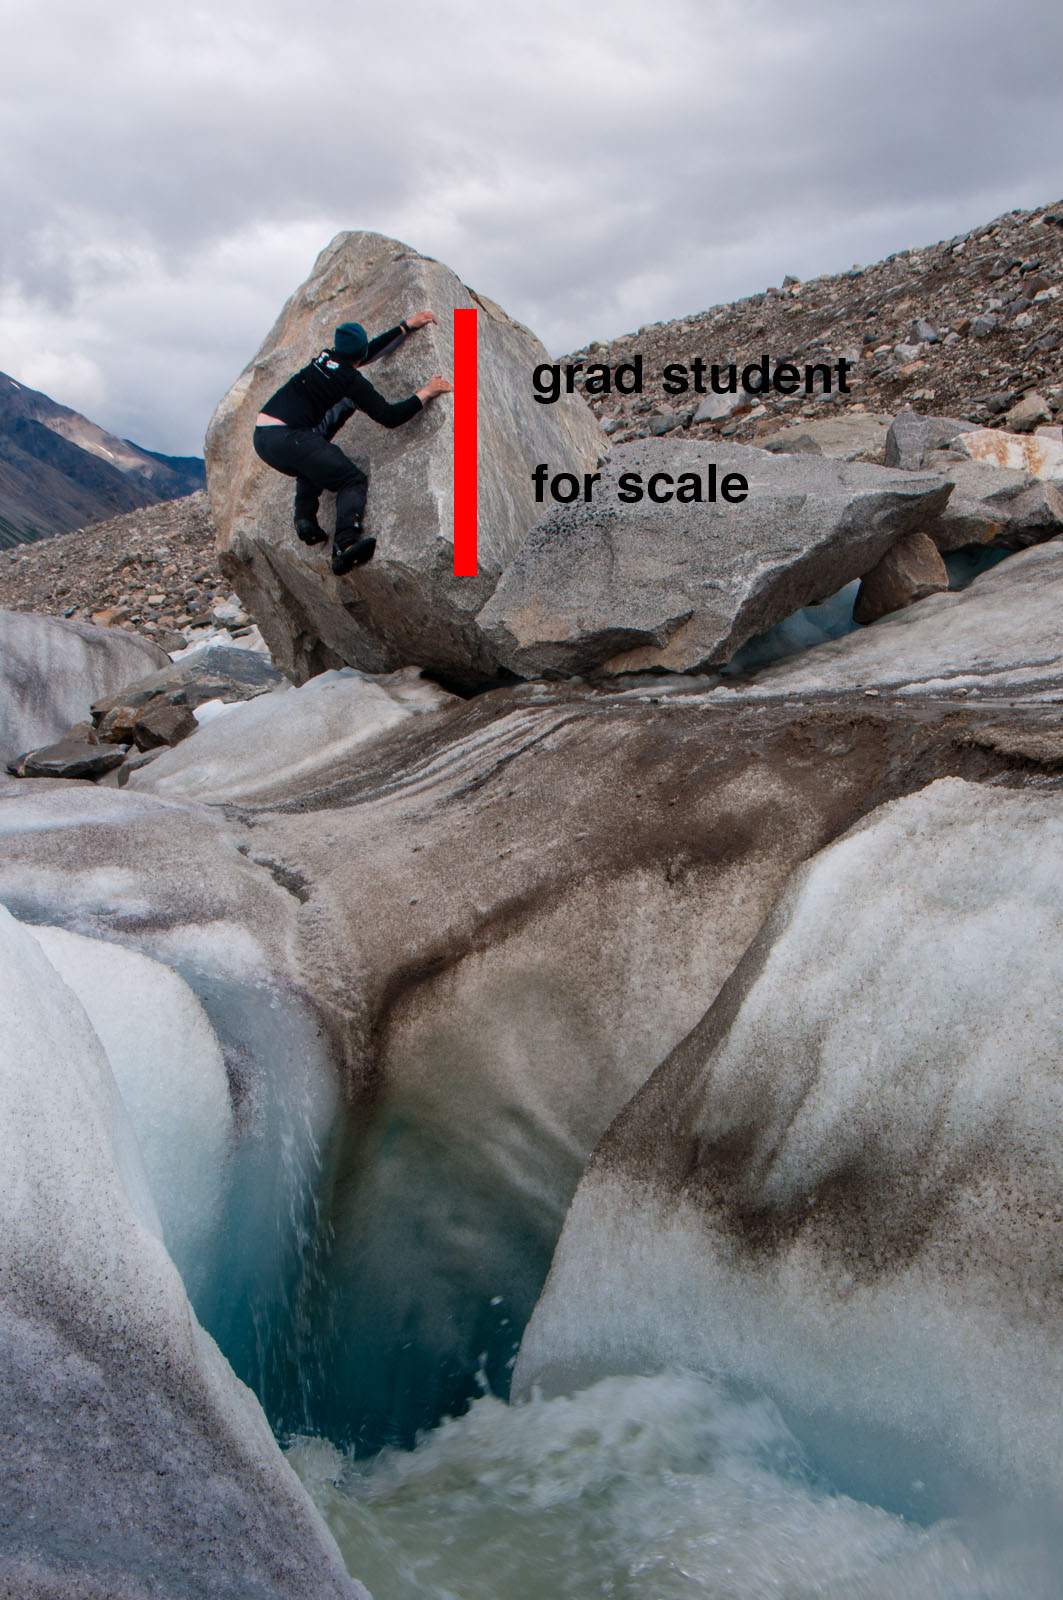
\includegraphics[height=5cm]{black-rapids-2}
  \end{figure}
  \begin{block}{Truffer's Law}
    \begin{itemize}
    \item whenever something interesting happens in a glacier, liquid water is involved
    \end{itemize}
  \end{block}
\end{frame}

\setbeamertemplate{background canvas}
  {
     \tikz{\node[inner sep=0pt,opacity=0.60] {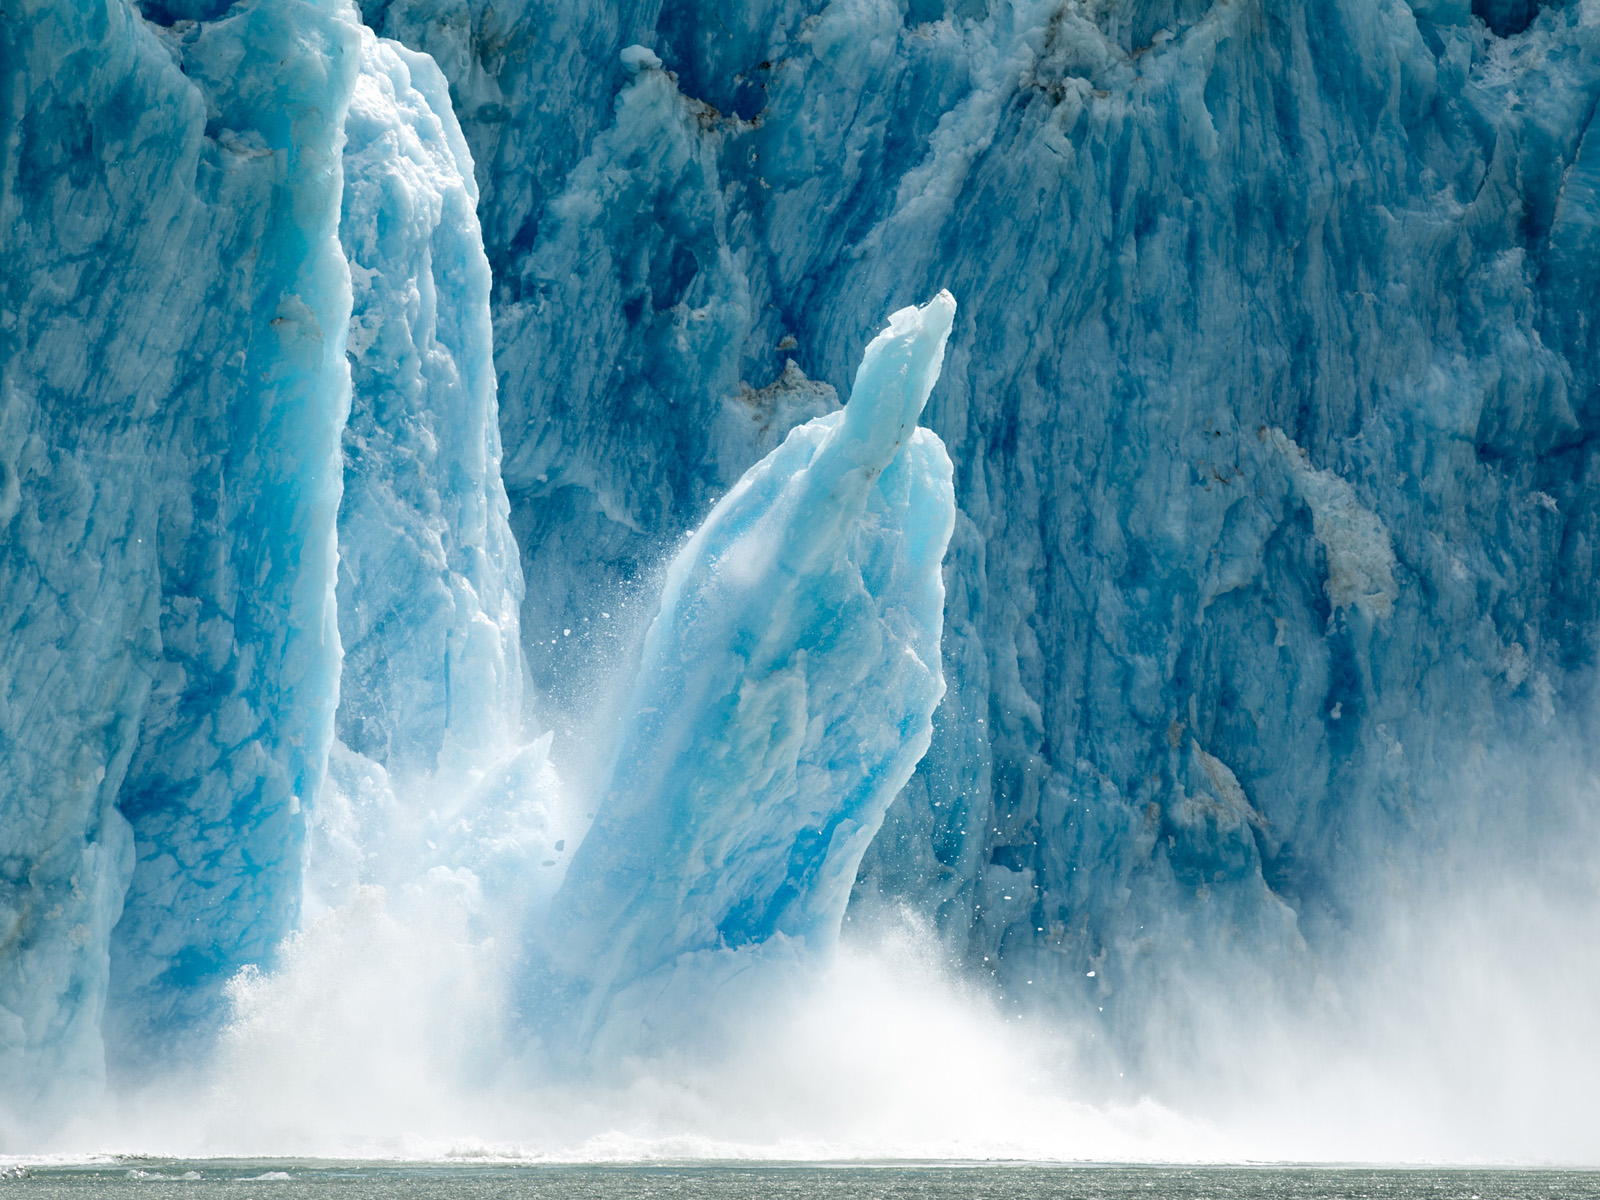
\includegraphics[height=
\paperheight,width=\paperwidth]{dawes_calving_alaska}};}
} 


\begin{frame}{The role of liquid water}
  \begin{columns}
    \column[C]{10cm}
    \begin{transbox}
      \begin{block}{at the lateral margin}
        \begin{columns}
          \column[C]{2.5cm}
          \begin{figure}
            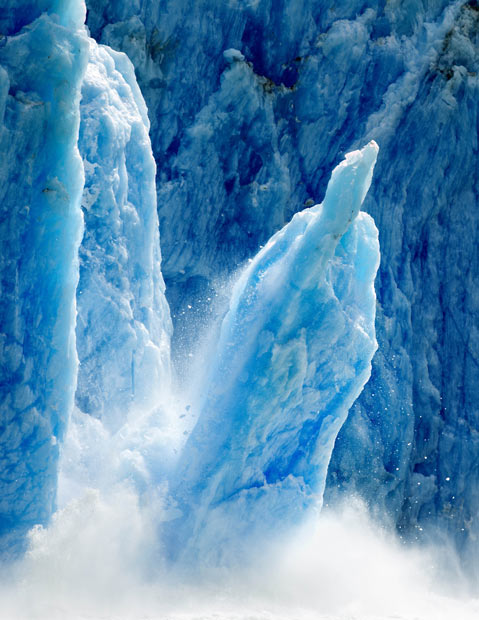
\includegraphics[width=\textwidth]{calving-close-up}
          \end{figure}
          \column[C]{7cm}
          drives calving and frontal melt of lake and ocean terminating glaciers\\
          lecture on \alert{tidewater glaciers and submarine melt} by Martin Truffer
        \end{columns}
      \end{block}
    \end{transbox}
  \end{columns}
\end{frame}

\begin{frame}{The role of liquid water}
  \begin{columns}
    \column[C]{10cm}
    \begin{transbox}
      \begin{block}{at the shelf base}
        \begin{columns}
          \column[C]{2.5cm}
          \begin{figure}
            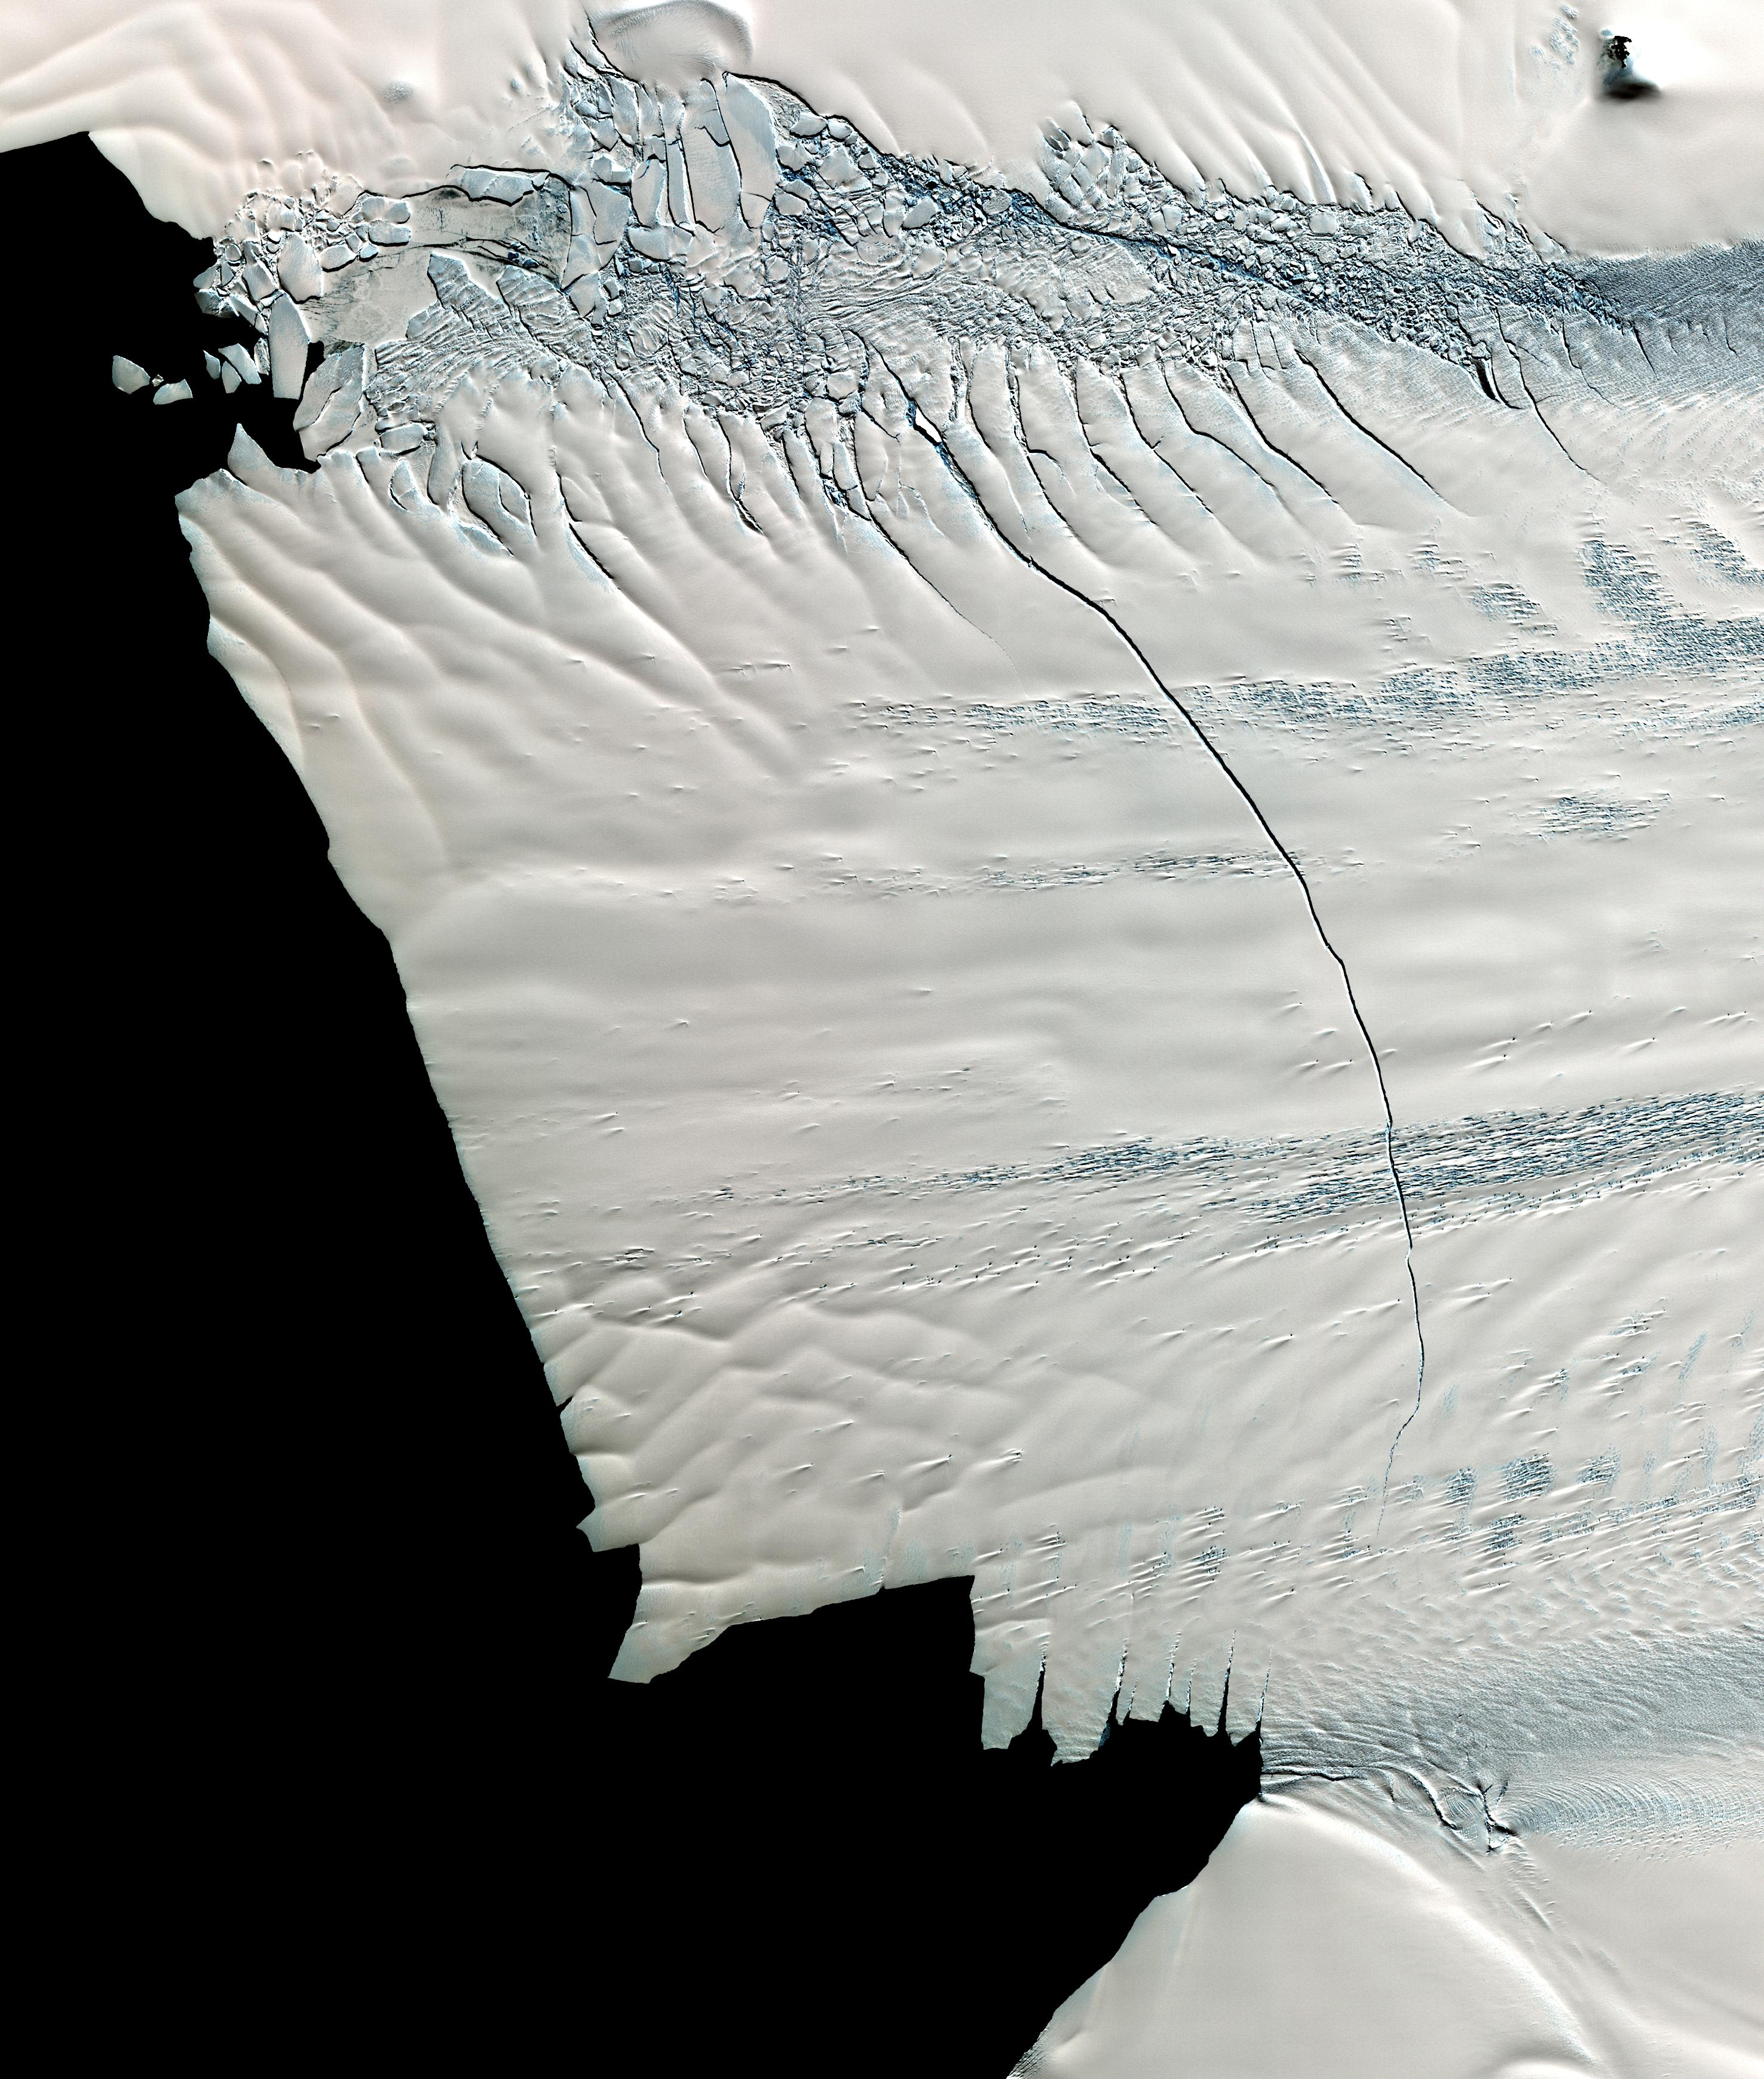
\includegraphics[width=\textwidth]{pig}
          \end{figure}
          \column[C]{7cm}
          attacks ice shelfs from below (sub-shelf basal melting) \\
          lecture on \alert{tidewater glaciers and submarine melt} by Martin Truffer
        \end{columns}
      \end{block}
    \end{transbox}
  \end{columns}
\end{frame}

\begin{frame}{The role of liquid water}
  \begin{columns}
    \column[C]{10cm}
    \begin{transbox}
      \begin{block}{at glacier base}
        \begin{columns}
          \column[C]{2.5cm}
          \begin{figure}
            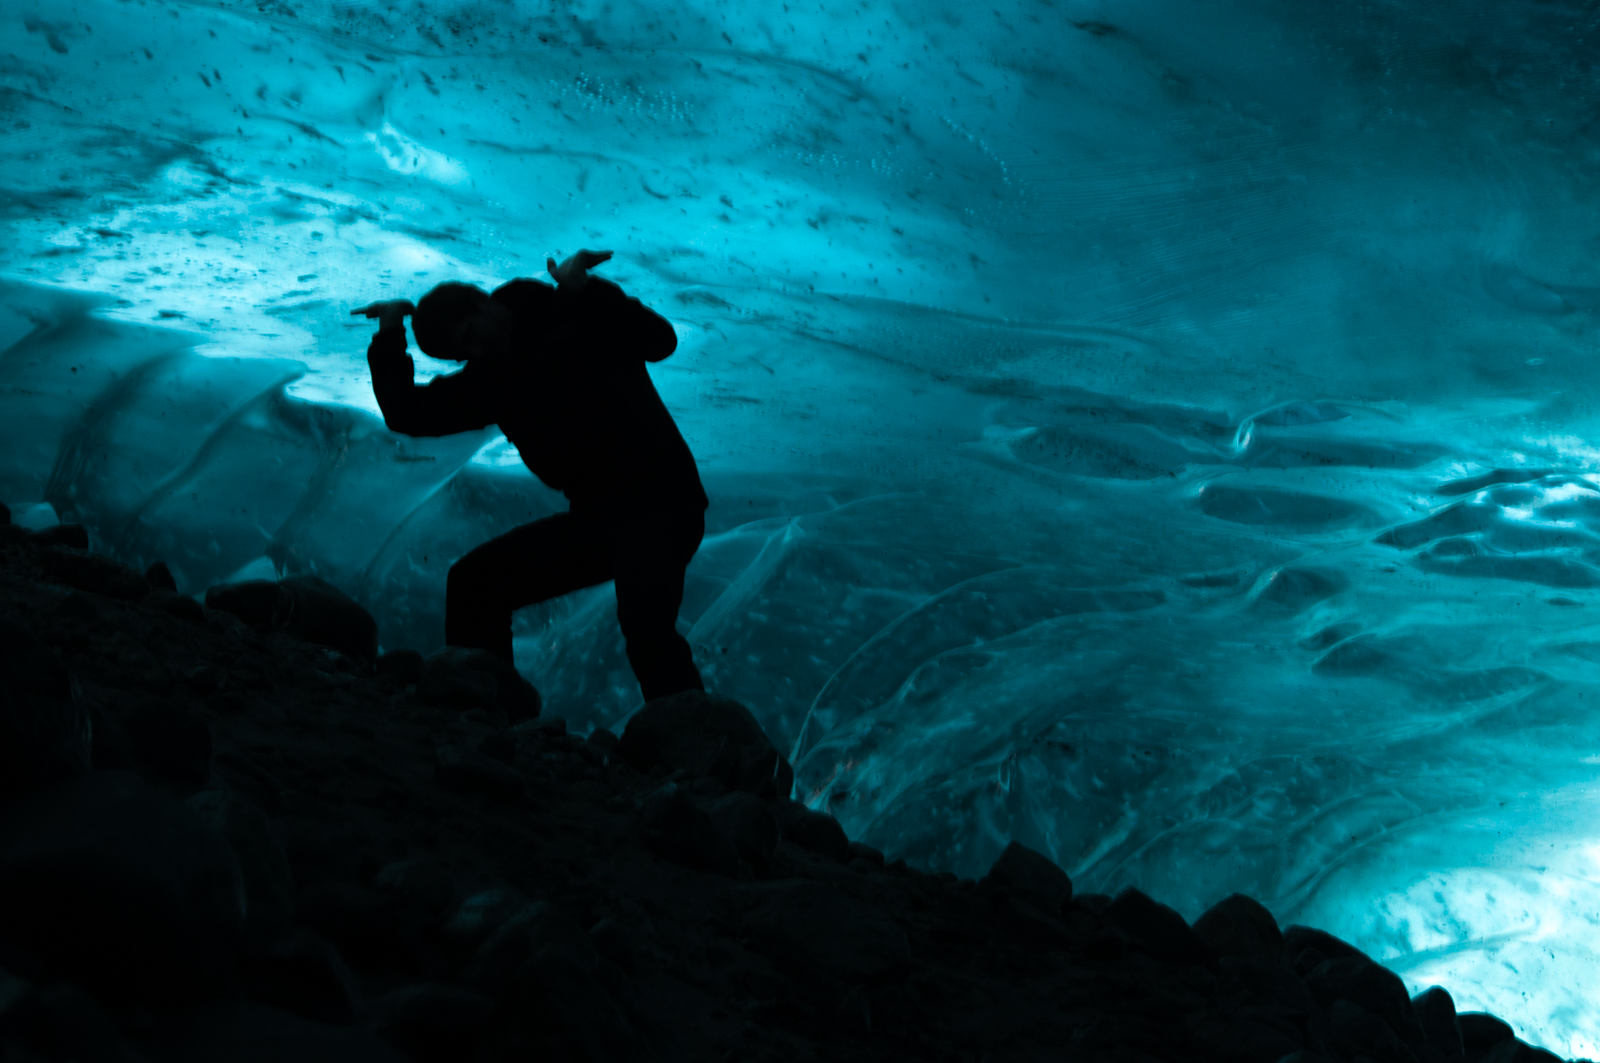
\includegraphics[width=\textwidth]{root-glacier-cave-1}
          \end{figure}
          \column[C]{7cm}
          acts as a lubricant at the base (sliding) \\
          lecture on \alert{subglacial hydrology} by Gwenn Flowers
          \\
          surging glaciers
        \end{columns}
      \end{block}
    \end{transbox}
  \end{columns}
\end{frame}



\begin{frame}{The role of liquid water}
  \begin{columns}
    \column[C]{10cm}
    \begin{transbox}
      \begin{block}{within temperate ice}
        \begin{columns}
          \column[C]{2.5cm}
          \begin{figure}
            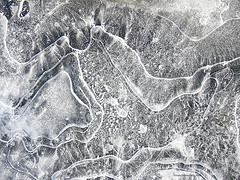
\includegraphics[width=\textwidth]{ice-matrix}
          \end{figure}
          \column[C]{7cm}
          softens the ice (decreases viscosity) \\
          lecture on \alert{thermodynamics} by Andy
        \end{columns}
      \end{block}
    \end{transbox}
  \end{columns}
\end{frame}

\setbeamertemplate{background canvas}
{
%
} 

%% \section[A Brief History]{A brief history of glacier flow}

%% \begin{frame}
%%   \frametitle{The role of water}
%%       In 1779, H.~B. de~Saussure observes sliding
%%       \begin{itemize}
%%         \item ``\ldots the weight of the ice might be sufficient to urge it down the slope of the valley, if the sliding motion were aided by the water flowing at the bottom.''
%%       \end{itemize}
%% \end{frame}

%% \begin{frame}
%%   \frametitle{The ``Hugi'' block}
%%   \begin{columns}
%%     \column[C]{4.25cm}
%%   \begin{figure}
%%     \includegraphics<1>[width=4cm]{hugi-block-boulder-movement-1}%
%%     \includegraphics<2>[width=4cm]{hugi-block-boulder-movement-2}%
%%     \includegraphics<3->[width=4cm]{hugi-block-boulder-movement-3}%
%%   \end{figure}
%%     \column[C]{7.75cm}
%%   \begin{figure}
%%     \includegraphics<1>[width=7cm]{glacier_flow_boulder_1}%
%%     \includegraphics<2>[width=7cm]{glacier_flow_boulder_2}%
%%     \includegraphics<4>[width=7cm]{glacier_flow_boulder_3}%
%%     \includegraphics<3>[width=7cm]{glacier_flow_boulder_4}%
%%   \end{figure}
%%   \end{columns}
%%   \visible<3->
%%       {\begin{block}{}
%%       J.~Hugi observed that a boulder moved $1315\,\text{m}$ downstream between 1827 and 1836
%%       \begin{itemize}
%%         \item<3> but back then, some people argued that a boulder slides on the glacier surface, the glacier itself is      \item<4> we would interpret this as clear evidence of glacier flow
%% motionless
%%       \end{itemize}
%%   \end{block}}
%% \end{frame}


%% \begin{frame}
%%   \frametitle{1840-1846 Dilatation theory by L. Agassiz}
%%   \begin{figure}
%%     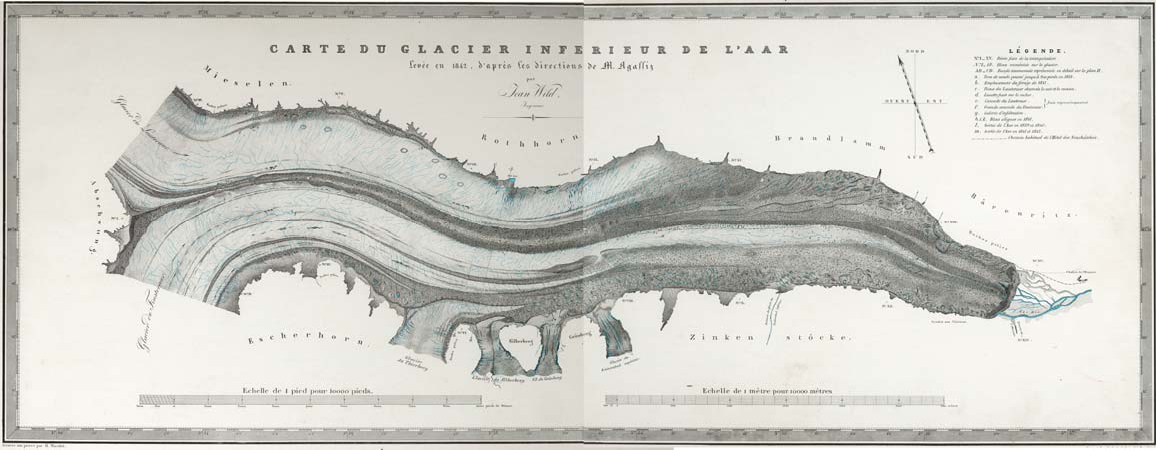
\includegraphics[width=8cm]{agassi}%
%%   \end{figure}
%%       \begin{itemize}
%%         \item glacier ice contains innumerable fissures and capillary tubes
%%         \item during the day, these tubes absorb the water
%%         \item and during the night, the water freezes
%%         \item this distension exerts a force and propels the glacier in the direction of least resistance
%%       \end{itemize}
%% \end{frame}


%% \begin{frame}
%%   \frametitle{1864-1930 Viscous flow theory by J.~Forbes$^*$}
%%   $^*$\emph{Abb{\'e} Rendu (Th{\'e}orie des glaciers de la Savoie, 1841) was the first to propose viscous flow}
%%   \begin{columns}
%%     \column[C]{4.2cm}
%%     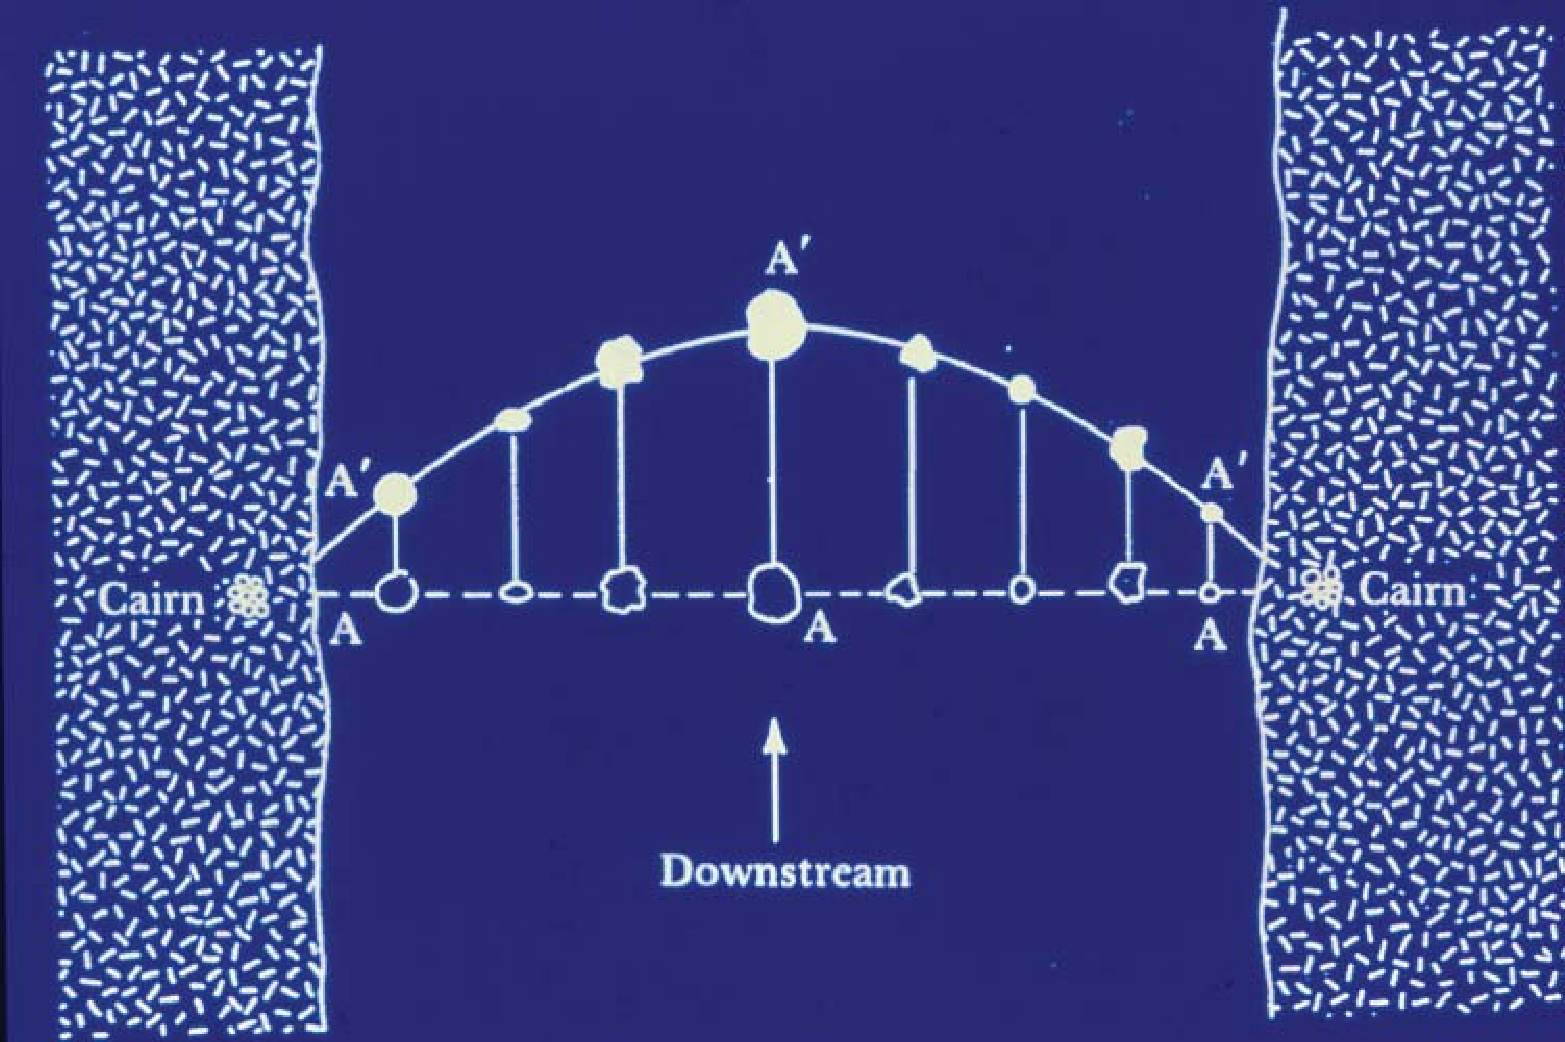
\includegraphics[width=3.8cm]{geschw_prof_oberfl}%
%%     \vskip1em
%%     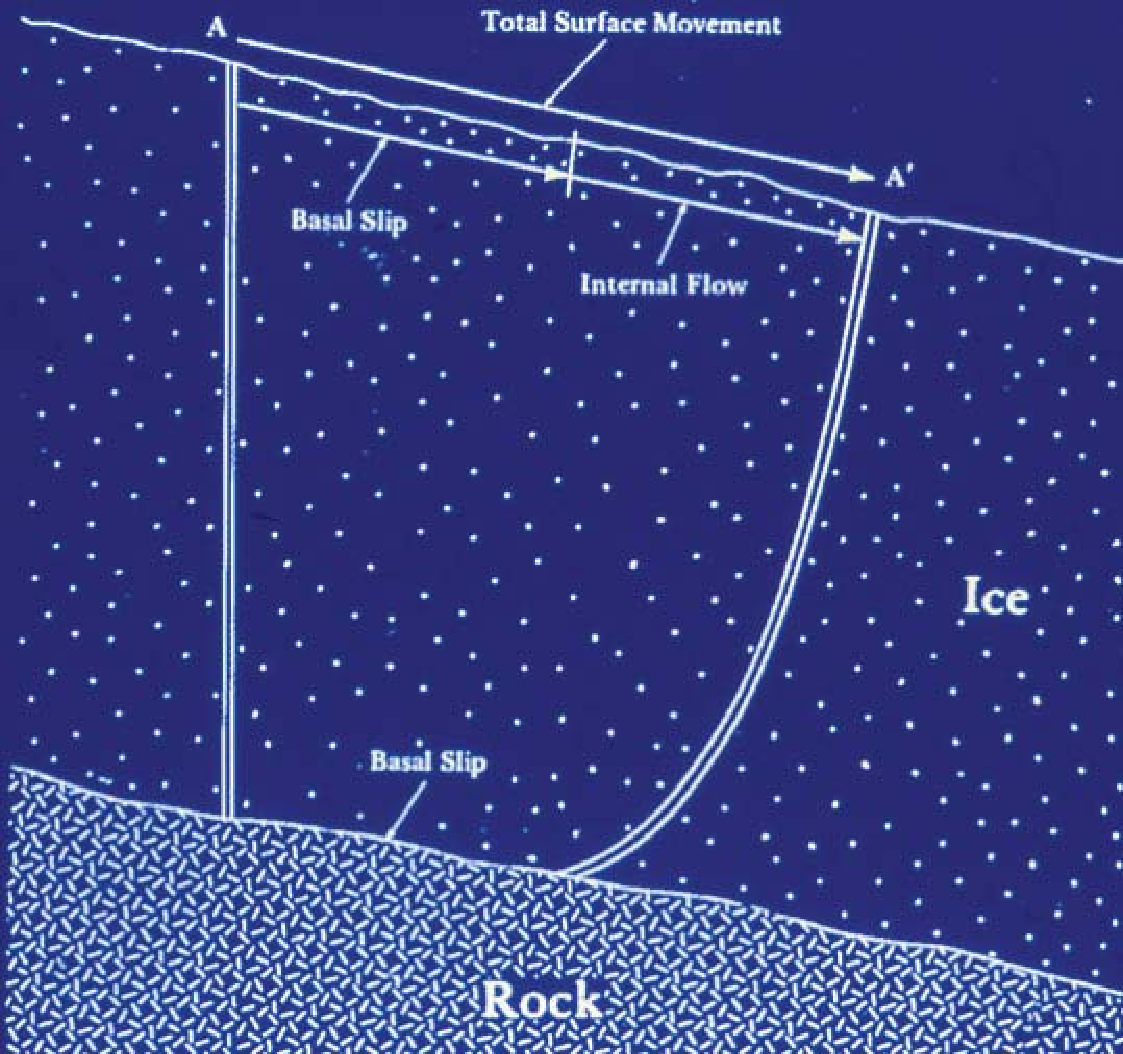
\includegraphics[width=3.8cm]{geschw_vert_prof}%
%%     \column[C]{7.8cm}
%%       \begin{itemize}
%%       \item made his own observations on Mer de Glace, France
%%       \item glacier flows fastest in the center
%%       \item opposes Agassi's theory
%%       \item if the dilatation theory were true
%%       \item then flow would be greatest at sunset
%%       \item and near the glacier margins
%%       \end{itemize}
%%   \end{columns}
%% \end{frame}




%% \begin{frame}{Forces}
%%   \begin{itemize}
%%   \item a force is a push or pull upon an object resulting from the object's interaction with another object
%%   \item whenever there is an interaction between two objects, there is a force upon each of the objects. 
%%   \end{itemize}
%%   In other words
%%   \begin{itemize}
%%   \item a force is any influence that causes an object to undergo a change in speed, a change in direction, or a change in shape
%%   \item forces exist inside continuous bodies such as a glacier
%%   \item these forces can cause a glacier to deform
%%   \end{itemize}
%% \end{frame}

%% \begin{frame}{What is stress?}
%%   ``Stress'' is the force per unit area acting on a material
%%   \begin{displaymath}
%%     \sigma = \frac{F}{A}
%%   \end{displaymath}
%%   Inside a glacier, stresses are due to
%%   \begin{itemize}
%%   \item weight of the overlying ice (overburden pressure)
%%   \item shape of the glacier surface (pressure gradients)
%%   \end{itemize}
%% \end{frame}


%% \begin{frame}{Types of stress}
%%   As a force per unit area, stress has a direction
%%   \begin{columns}
%%     \column[c]{5cm}
%%     \begin{figure}
%%       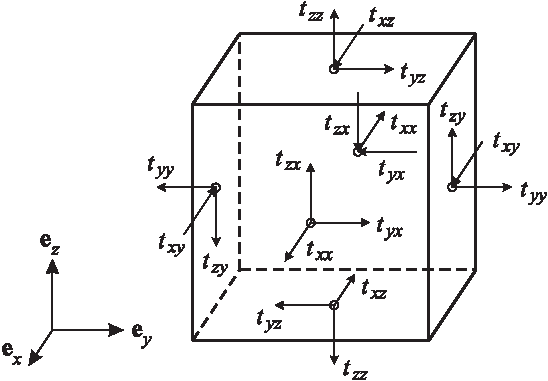
\includegraphics[width=4.75cm]{fig_3_08}
%%     \end{figure}
%%     \column[c]{6.5cm}
%%    \begin{block}{}
%%       Force can be directed normal to the area
%%       \begin{itemize}
%%       \item Result is \alert{pressure} if the force is the same on all faces of a cube.
%%       \item Result is \alert{normal stress} if forces are different on different faces
%%       \end{itemize}
%%     \end{block}
%%     \begin{block}{} 
%%       Force can be directed parallel to the area
%%       \begin{itemize}
%%       \item Result is \alert{shear stress}
%%       \end{itemize}
%%     \end{block}
%%   \end{columns}
%% \end{frame}

\begin{frame}{Pressure in a glacier}
  mass $m = \rho V$
     \begin{itemize}
      \item $\rho$ = ice density $\approx$ 900\,kg\,m$^{-3}$
      \item$V$ = Volume = Area $\times$ depth = $A \cdot h$
     \end{itemize}
     So pressure $p$ at depth $h$ is
     \begin{displaymath}
       p = \frac{m \cdot g}{A} = \frac{\rho \cdot A \cdot h \cdot g}{A} = \rho g h + p_{\textsf{air}}
     \end{displaymath}
     How deep do we have to drill into a glacier before the ice pressure is 2 atmosphere?
\end{frame}


\begin{frame}{Depth for 2\,atm pressure?}
    \begin{displaymath}
       h = \frac{p-p_{\textsf{air}}}{\rho\cdot g} = ?
     \end{displaymath}
     \begin{itemize}
     \item  So pressure rises by 1\,atm for every \alert{$x$}\,meters of depth in a glacier
     \item Does ice deform in response to this pressure?
     \end{itemize}
\end{frame}


\begin{frame}{Shear stress $\tau$}
  Total stress $t$ from ice column:
    \begin{displaymath}
       t = \frac{\rho V g}{A} = \rho\,g\,h
     \end{displaymath}
     \begin{itemize}
     \item How much of this weight will contribute to shear deformation?
     \item shear stress $\tau = \rho\,g\,h\,\sin{\alpha}$
     \item normal stress $\sigma = \rho\,g\,h\,\cos{\alpha}$
    \end{itemize}
\end{frame}


\begin{frame}{Shear stress in a glacier}
\begin{columns}[c]
  \begin{column}{.5\textwidth}
    \begin{block}{Valley Glacier}
      \begin{itemize}
      \item $h$ = 130\,m
      \item $\alpha$ = 5$^{\circ}$
      \end{itemize}
    \end{block}
  \end{column}
  \begin{column}{.5\textwidth}
    \begin{block}{Ice Sheet}
  \begin{itemize}
  \item $h$ = 1300\,m
  \item $\alpha$ = 0.5$^{\circ}$
  \end{itemize}
\end{block}
\end{column}
\end{columns}
\vspace{1em}
\begin{displaymath}
    \tau = \rho\,g\,h\,\sin{\alpha}
  \end{displaymath}
  \begin{beamercolorbox}[rounded=true,shadow=true]{boxed}
    Shear stress at the glacier base, $\tau_{b}$, is $\approx$ 1\,bar, which is a typical value for basal shear stress under a glacier
  \end{beamercolorbox}
\end{frame}
   

\begin{frame}{Are glacier thickness and slope related?}
  Suppose a glacier becomes thicker or steeper due to mass imbalance:
  \begin{itemize}
    \item it flows faster
    \item it quickly reduces thickness $h$ or slope $\alpha$, until $\tau_{b} \approx$ 1\,bar again
  \end{itemize}
  Can we then estimate glacier thickness ($z=h$) from its slope if we know $\tau_{b} \approx$ 1\,bar?
  \begin{displaymath}
    \tau = \rho\,g\,h\,\sin{\alpha} \quad \Rightarrow \quad h \sim \frac{\tau_{b}}{\rho\,g\,\sin{\alpha}}
  \end{displaymath}
\end{frame}


\begin{frame}{An ice sheet of infinite height?}
\begin{itemize}
  \item power-law stress-strain relationship $\Rightarrow$ ice softens
    rapidly as the shear stress exceeds 1\,bar.
  \item ice flow also increases rapidly $\Rightarrow$ glacier expands
    and thins
  \item that 1\,bar is a typical stress is a result of $A$ and $n$
\end{itemize}

\end{frame}


%% \begin{frame}{A Recipe}
%%   A recipe to calculate the flow velocities from given stresses, strain rates, symmetry conditions and
%%   boundary conditions
%%   \begin{enumerate}
%%   \item determine all components of the stress tensor $\sigma_{ij}$
%%     exploiting the symmetries, and using the flow law
%%   \item calculate the mean stress $\sigma_m$
%%   \item calculate the deviatoric stress tensor $\sigma^{(d)}_{ij}$
%%   \item calculate the effective shear stress (second invariant) $\tau$
%%   \item calculate the strain rates $\epsdot_{ij}$ from $\tau$ and
%%     $\sigma^{(d)}_{ij}$ using  the flow law
%%   \item integrate the strain rates to obtain velocities
%%   \item insert boundary conditions
%%   \end{enumerate}
%% \end{frame}



%% \begin{frame}{Why ice sheet modeling is easy}
%%   \begin{columns}[c]
%%     \begin{column}{.28\linewidth}
%%       \begin{figure}
%%         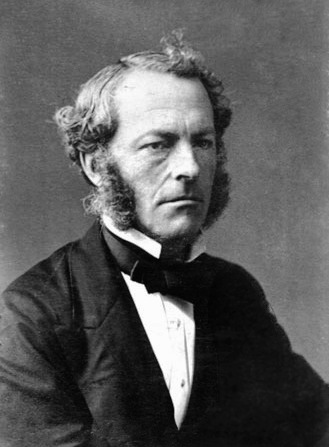
\includegraphics[width=\linewidth]{ggstokes}
%%         \\ \scriptsize{G.~G.~Stokes}
%%       \end{figure}
%%     \end{column}
%%     \begin{column}{.67\linewidth}
%%       \begin{itemize}[<+- | alert@+>]
%%       \item composed of a single, largely homogeneous material
%%       \item flow governed by the Stokes equations known since the mid-19th century
%%       \item flows slowly: we can ignore turbulence, Coriolis and other inertial effects
%%       \item no density/salinity stratification
%%       \item most of what makes atmosphere and ocean flow interesting is missing
%%       \end{itemize}
%%     \end{column}
%%   \end{columns}
%% \end{frame}

%% \begin{frame}{On turbulence}
%%   \begin{beamercolorbox}[rounded=true,shadow=true]{boxed}
%%     ``I am an old man now, and when I die and go to heaven there are two matters on which I hope for enlightenment. One is quantum electrodynamics, and the other is the turbulent motion of fluids. And about the former I am rather optimistic.'' (O.~Reynolds)
%%   \end{beamercolorbox}
%%   \begin{itemize}
%%   \item so what makes the flow of slow, cold, laminar ice interesting?
%%   \end{itemize}
%% \end{frame}


%% \begin{frame}{Why ice sheet modeling is so hard}
%%     \begin{columns}[c]<1-2>
%%       \begin{column}{.28\linewidth}
%%         \begin{figure}
%%           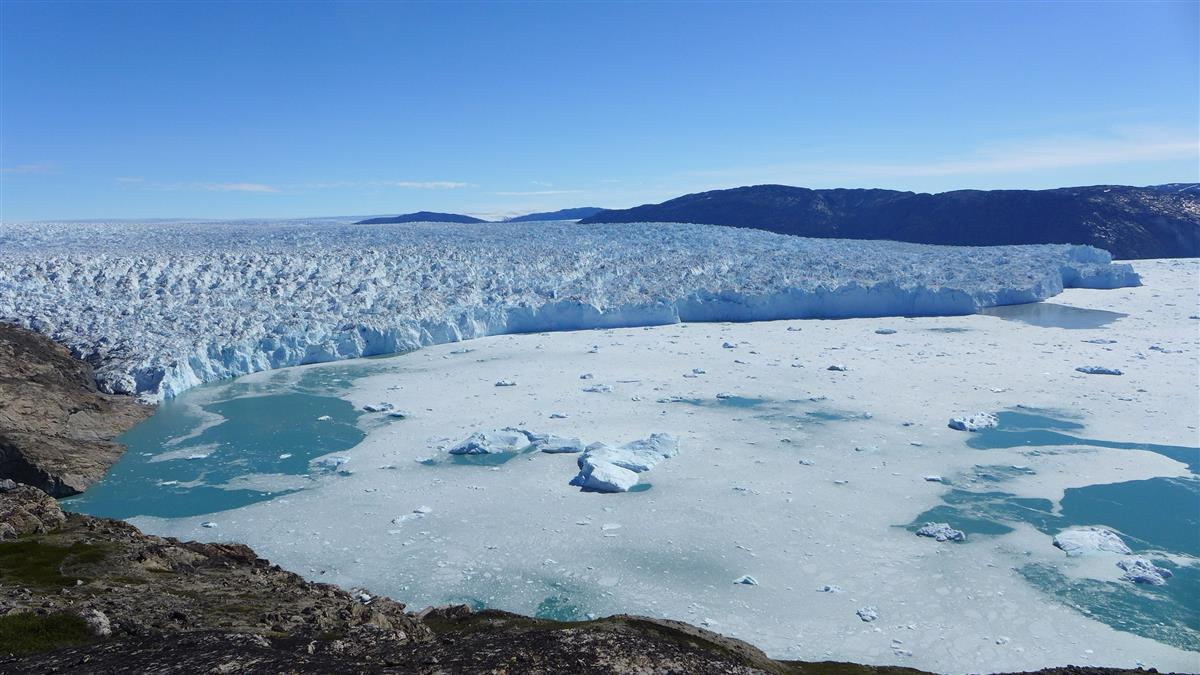
\includegraphics[width=\linewidth]{storeglacier}
%%         \end{figure}
%%       \end{column}
%%       \begin{column}{.67\linewidth}
%%         \begin{block}{Boundary conditions}
%%         \begin{itemize}
%%         \item seaward margin boundary condition
%%         \item basal boundary condition
%%         \end{itemize}
%%       \end{block}
%%       \end{column}
%%     \end{columns}
%%     \begin{columns}[c]<1>
%%       \begin{column}{.28\linewidth}
%%         \begin{figure}
%%           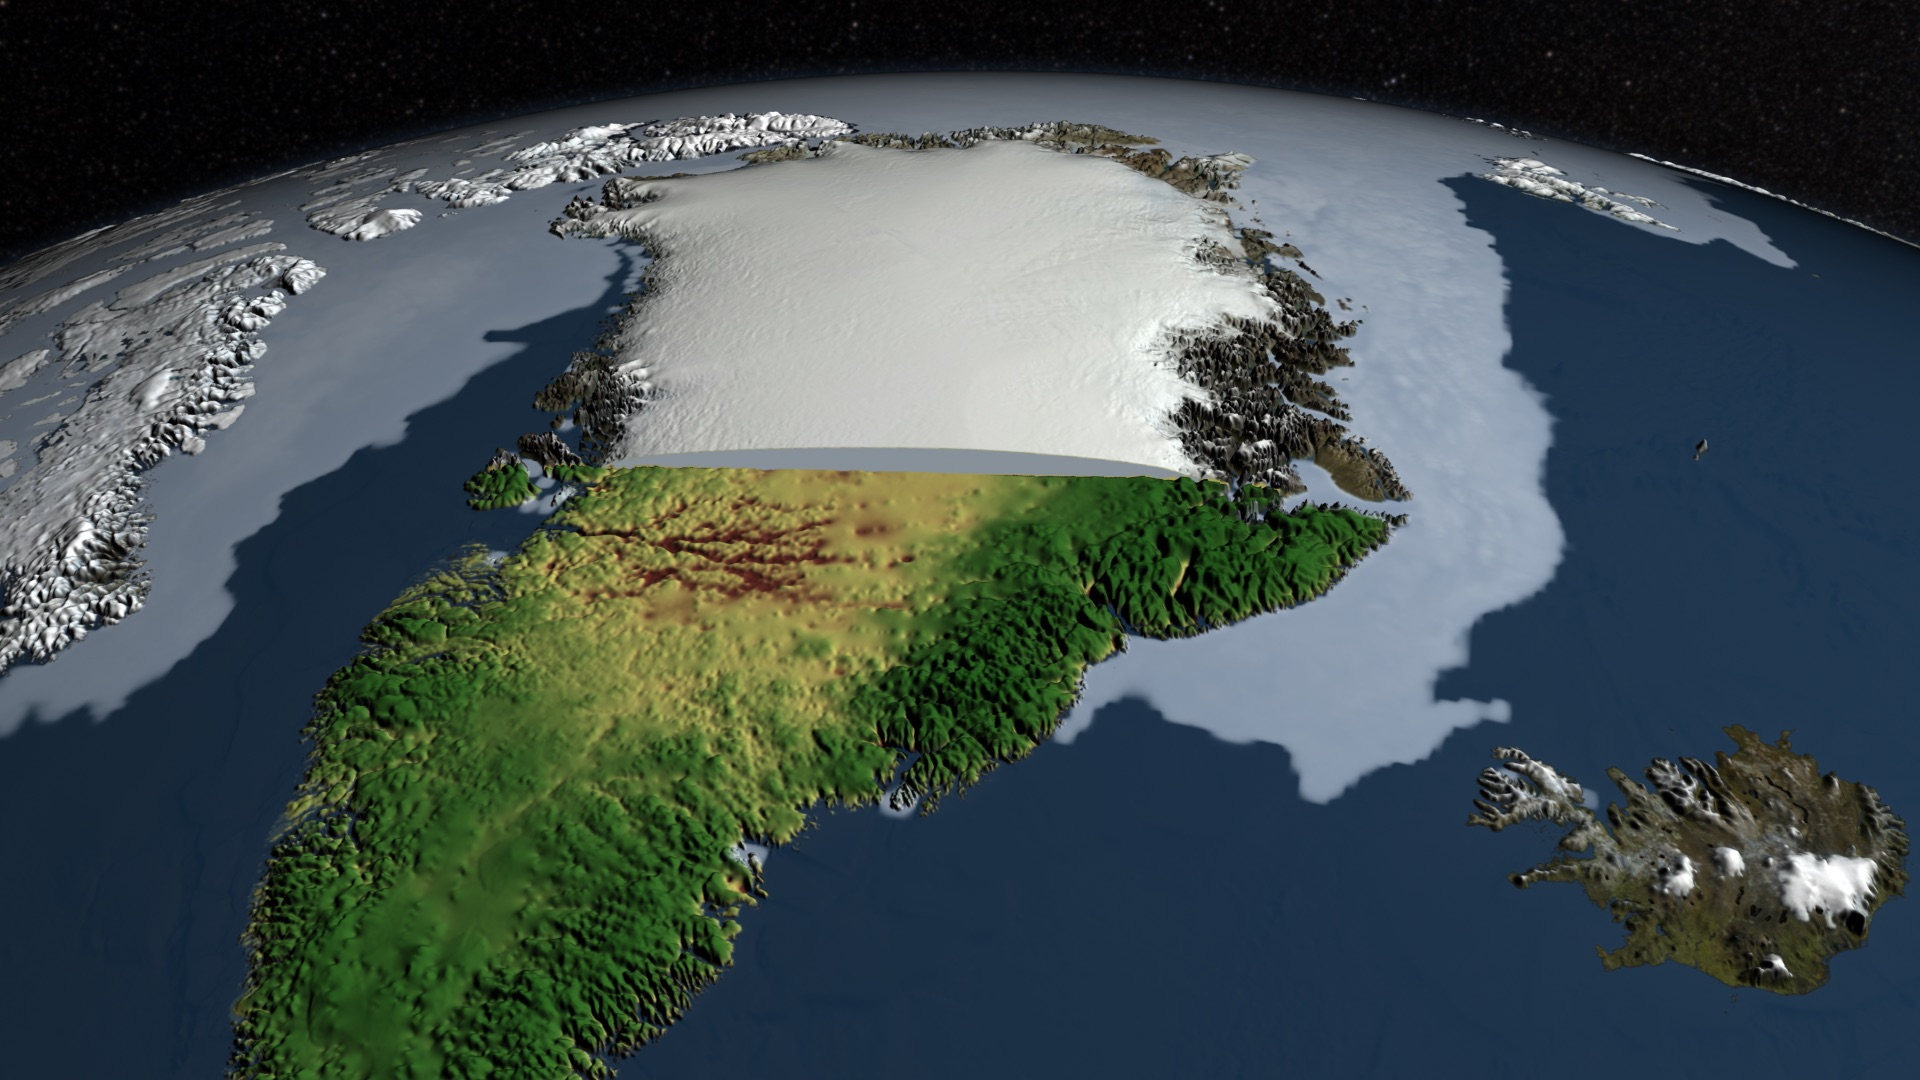
\includegraphics[width=\linewidth]{canale_grande_V05}
%%         \end{figure}
%%       \end{column}
%%       \begin{column}{.67\linewidth}
%%         \begin{block}{Initial conditions}
%%         \begin{itemize}
%%         \item ice thickness / subglacial topography is a first order constraint on ice flow
%%         \end{itemize}
%%       \end{block}
%%       \end{column}
%%     \end{columns}
%%     \begin{columns}[c]<1>
%%       \begin{column}{.3\linewidth}
%%         \begin{figure}
%%           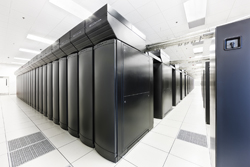
\includegraphics[width=\linewidth]{bw_front_sm}
%%         \end{figure}
%%       \end{column}
%%       \begin{column}{.67\linewidth}
%%         \begin{block}{Computational costs}
%%         \begin{itemize}
%%         \item solving the Stokes equations is computationally very expensive
%%         \end{itemize}
%%       \end{block}
%%       \end{column}
%%     \end{columns}
%% \end{frame}


%% \begin{frame}{Challenge: basal boundary condition}
%%   \begin{columns}[c]
%%     \begin{column}{.45\linewidth}
%%       \begin{figure}
%%         \scriptsize{basal resistance} \\
%%         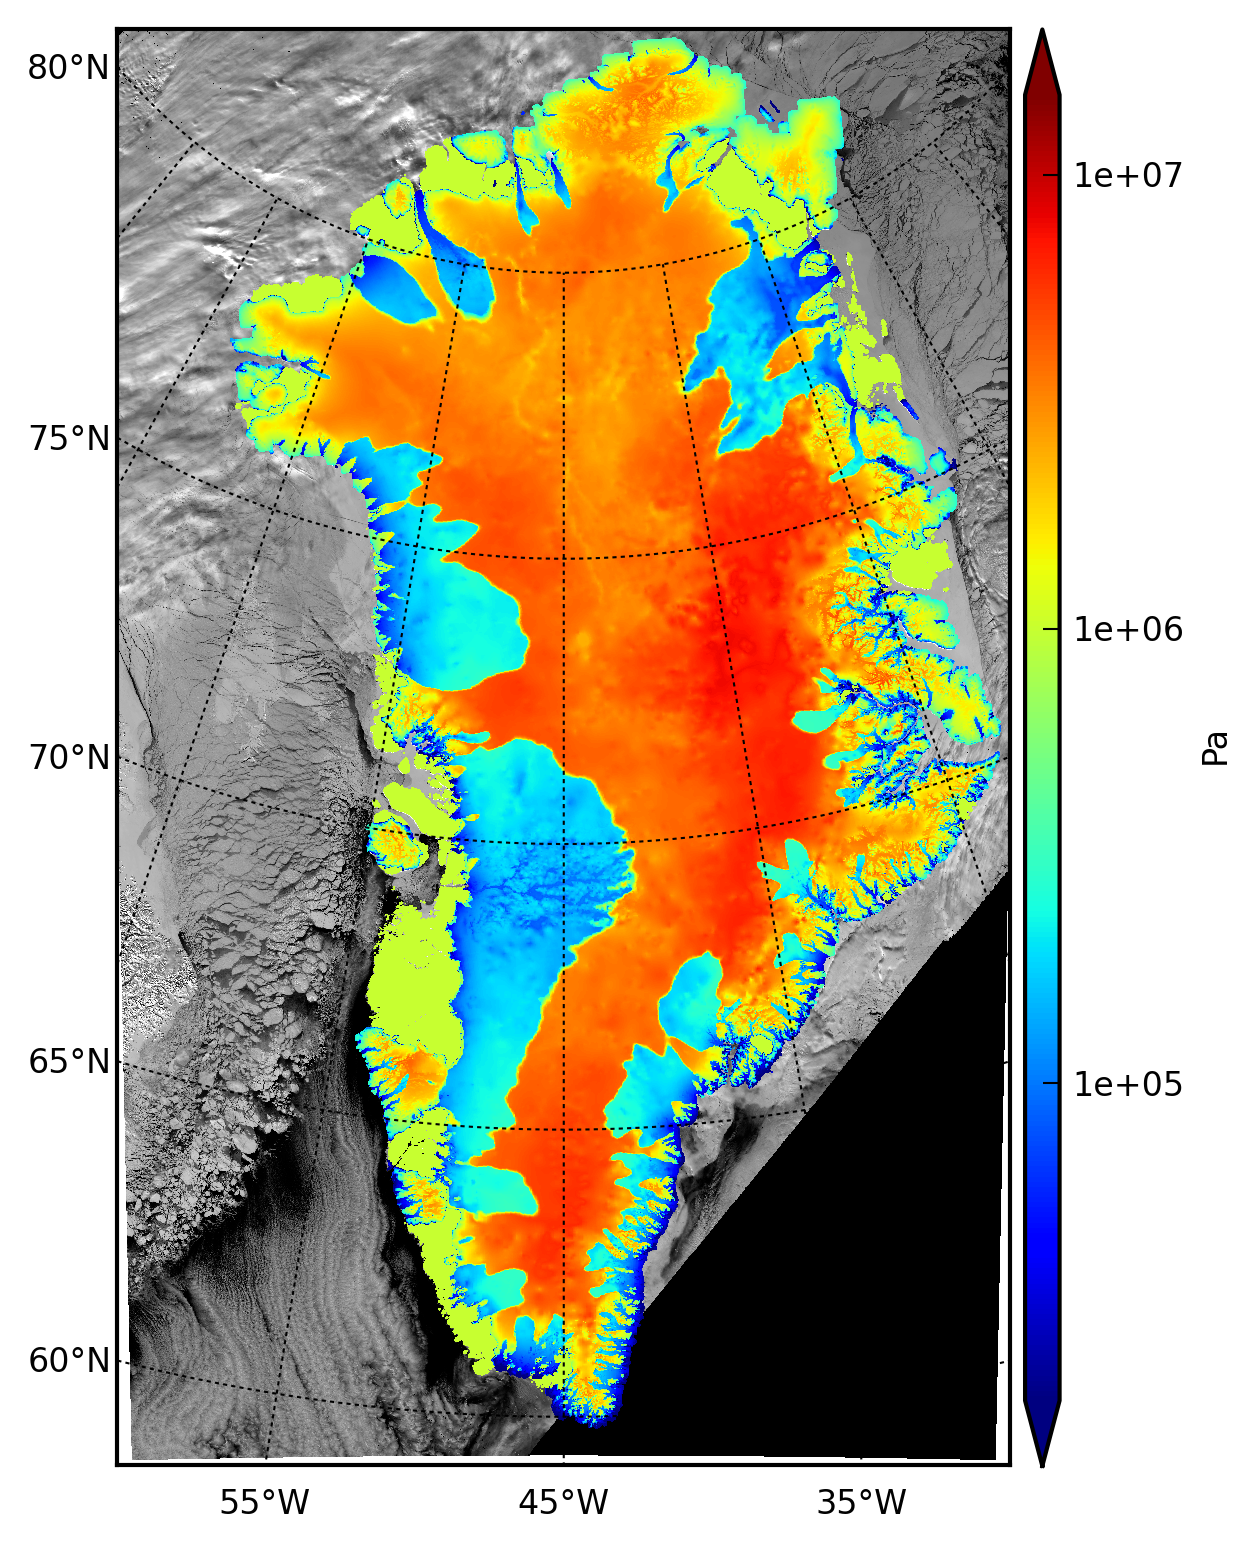
\includegraphics[width=\textwidth]{tauc}
%%       \end{figure}
%%     \end{column}
%%     \begin{column}{.54\linewidth}
%%       \begin{itemize}
%%       \item stresses vary by orders of magnitude
%%       \item basal hydrology, the glacier's ``plumbing system'' runs on a faster time scale than ice flow
%%       \item despite more than 5 decades of research, we only have crude parametrizations
%%       \item[$\Rightarrow$] Martin's inverse method lecture
%%       \end{itemize}
%%     \end{column}
%%   \end{columns}
%%   \note[item]{First, stresses at the base vary by several orders of magnitude}
%%   \note[item]{depend on many factors, most importantly on the presence or absence of water}
%%   \note[item]{basal hydrology (the glacier's plumbing system) runs on a faster time scale than the ice flow itself}
%%   \note[item]{but the sub-glacial environment is not easy accessible}
%%   \note[item]{at the basal boundary, interactions between water flow, friction, heat flow, and sediment deformation is so complex that a deriving a theory from first principles is real challenge}
%% \end{frame}


%% \begin{frame}{Challenge: seaward margin boundary condition}
%%       \begin{figure}
%%         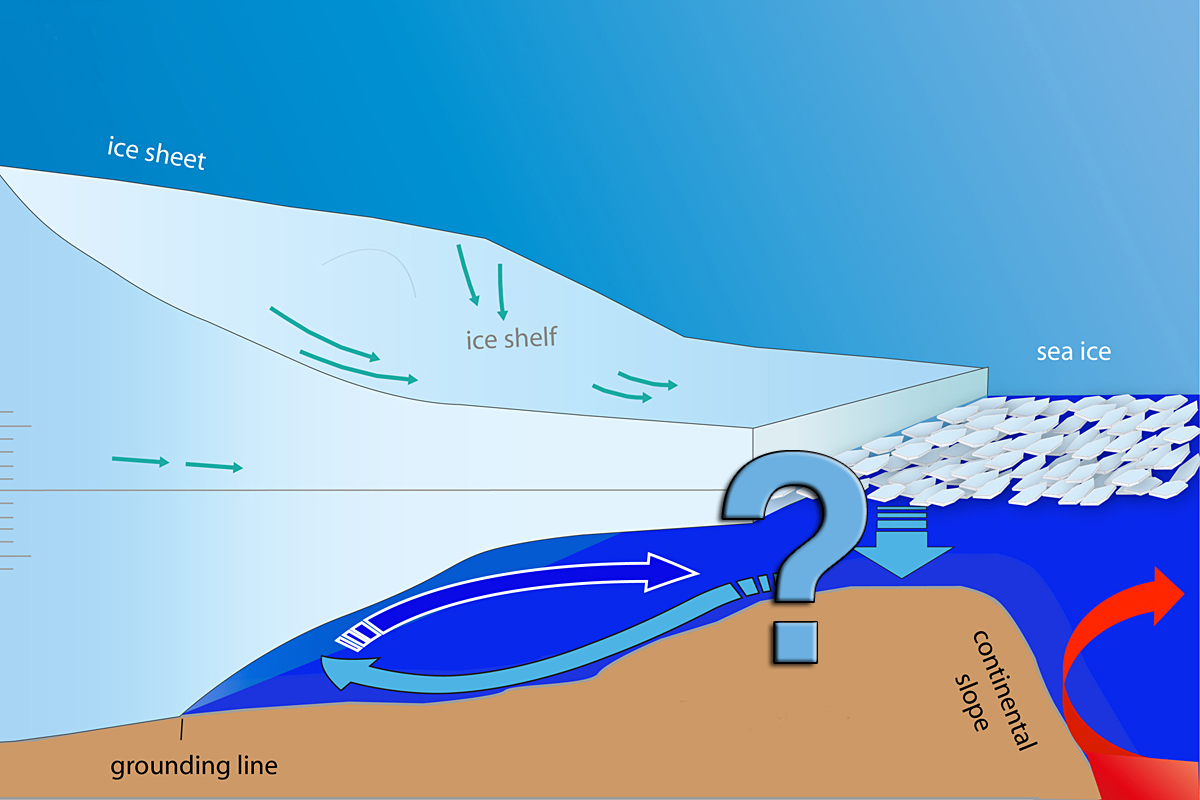
\includegraphics[width=.5\textwidth]{ice-shelf}
%%       \end{figure}
%%       \begin{itemize}
%%       \item ocean circulation $\Rightarrow$ basal melt rates
%%       \item calving mechanism
%%       \item[$\Rightarrow$] Martin's tidewater glacier lecture
%%       \end{itemize}
%%       \note[item]{a big challenge is to understand how changing ocean currents and ocean temperatures affects sub-shelf basal melt rates}
%%       \note[item]{how this can weaken a shelf, and potentially lead to break up}
%% \end{frame}


%% \begin{frame}{Why ice sheet modeling is so hard}
%%     \begin{columns}[c]<1>
%%       \begin{column}{.28\linewidth}
%%         \begin{figure}
%%           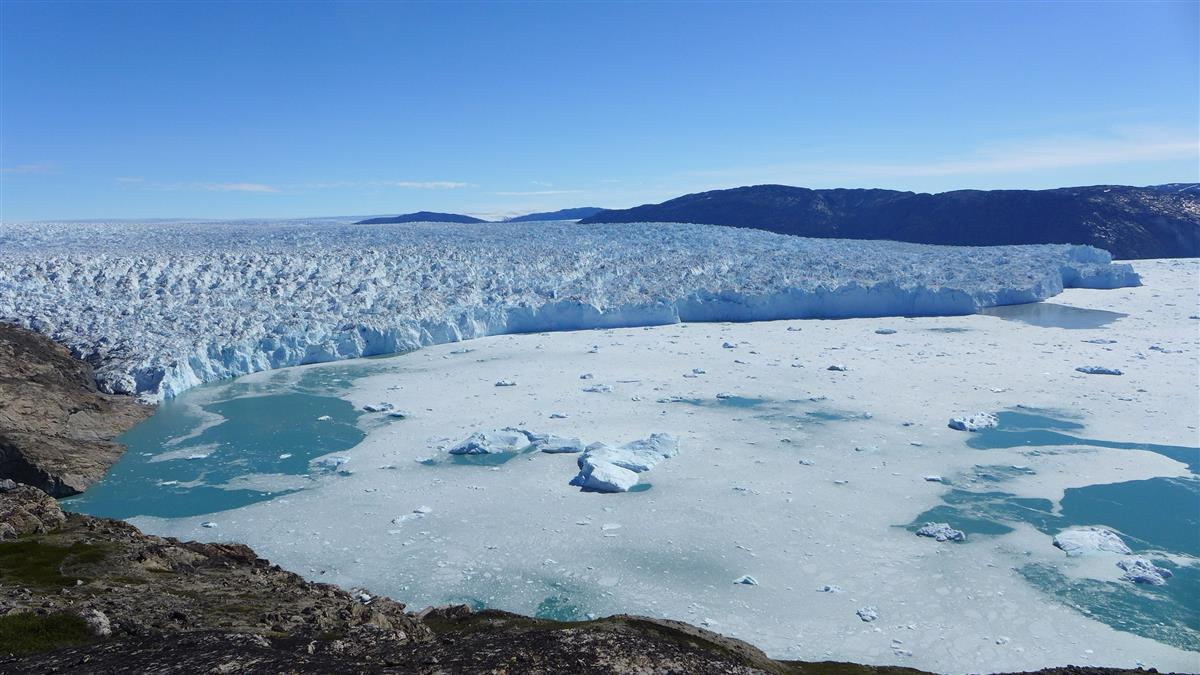
\includegraphics[width=\linewidth]{storeglacier}
%%         \end{figure}
%%       \end{column}
%%       \begin{column}{.67\linewidth}
%%         \begin{block}{Boundary conditions}
%%         \begin{itemize}
%%         \item seaward margin boundary condition
%%         \item basal boundary condition
%%         \end{itemize}
%%       \end{block}
%%       \end{column}
%%     \end{columns}
%%     \begin{columns}[c]<1-2>
%%       \begin{column}{.28\linewidth}
%%         \begin{figure}
%%           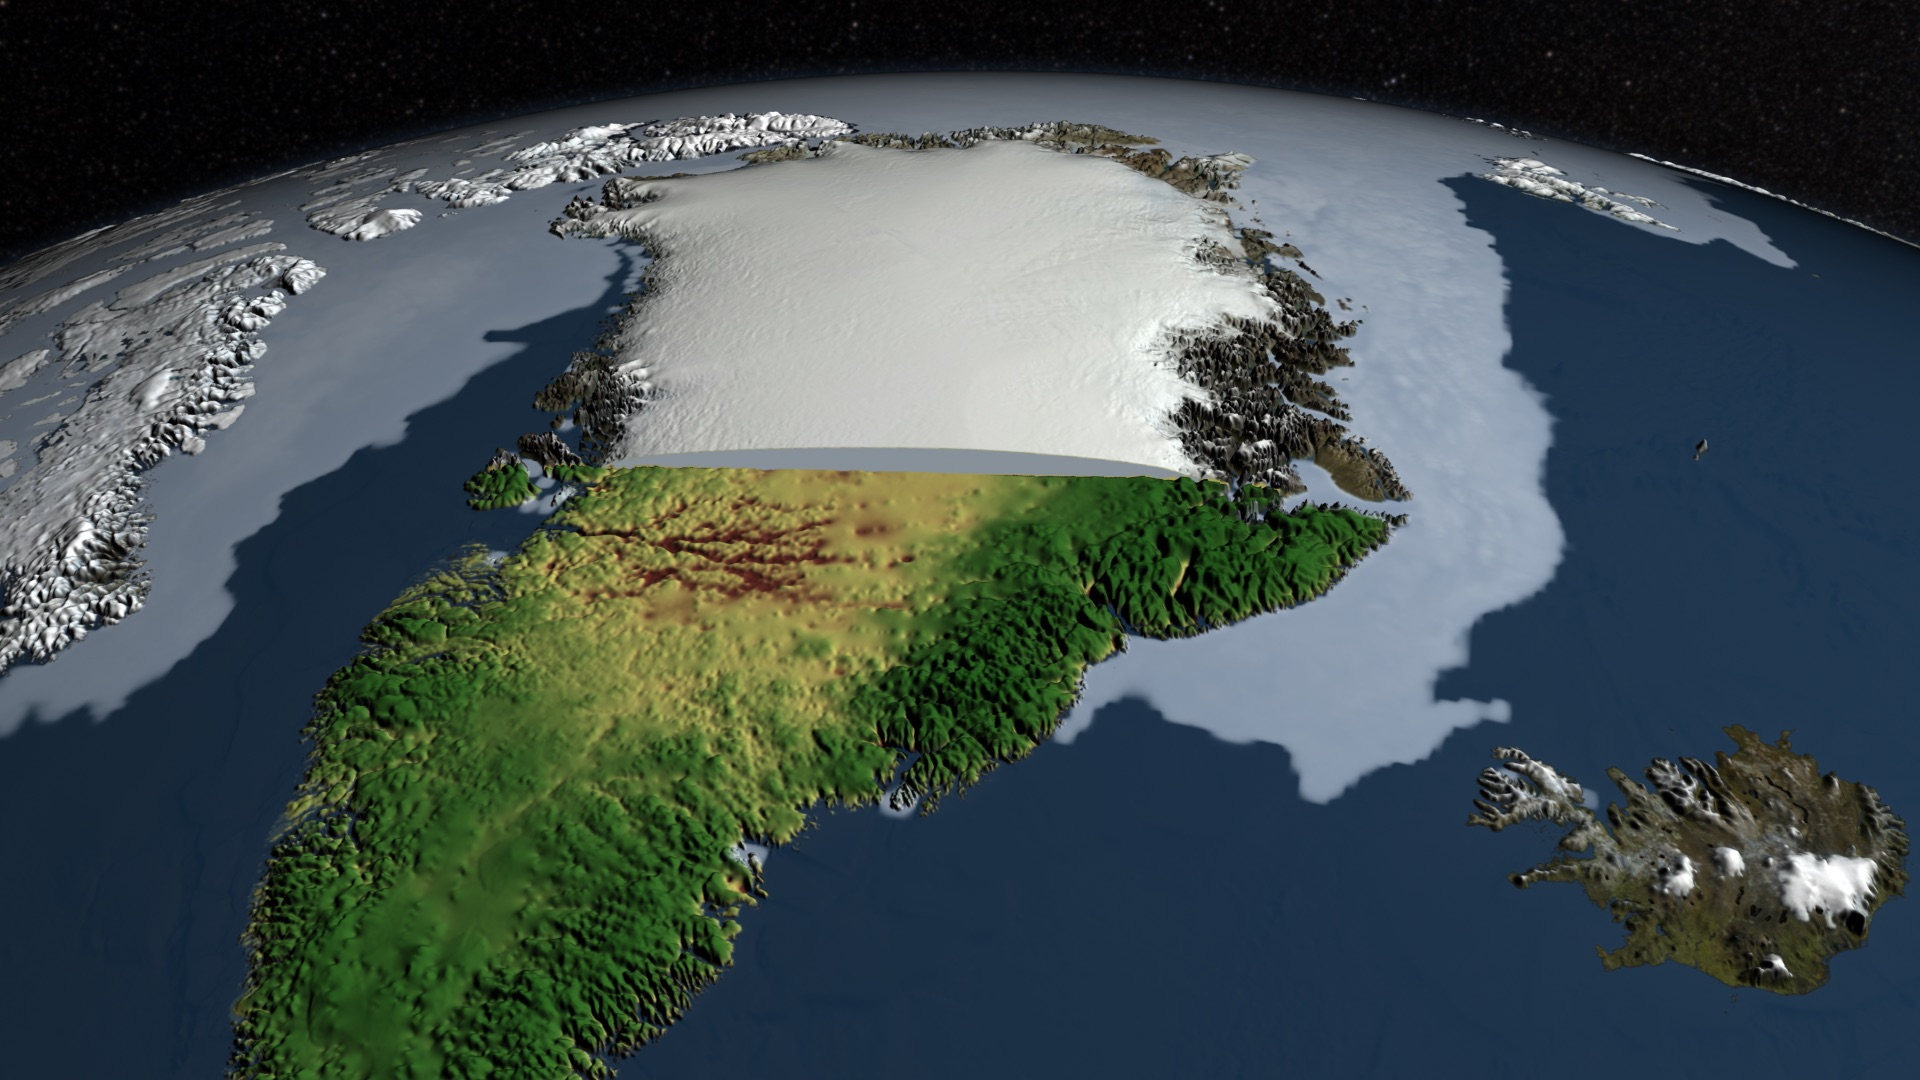
\includegraphics[width=\linewidth]{canale_grande_V05}
%%         \end{figure}
%%       \end{column}
%%       \begin{column}{.67\linewidth}
%%         \begin{block}{Initial conditions}
%%         \begin{itemize}
%%         \item ice thickness / subglacial topography is a first order constraint on ice flow
%%         \end{itemize}
%%       \end{block}
%%       \end{column}
%%     \end{columns}
%%     \begin{columns}[c]<1-3>
%%       \begin{column}{.3\linewidth}
%%         \begin{figure}
%%           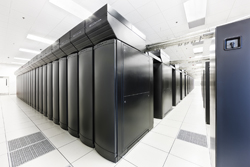
\includegraphics[width=\linewidth]{bw_front_sm}
%%         \end{figure}
%%       \end{column}
%%       \begin{column}{.67\linewidth}
%%         \begin{block}{Computational costs}
%%         \begin{itemize}
%%         \item solving the Stokes equations is computationally very expensive
%%         \end{itemize}
%%       \end{block}
%%       \end{column}
%%     \end{columns}
%% \end{frame}


%% \begin{frame}{1. Simplify the Stokes equations}
%%   \begin{block}{Ice sheets are shallow}
%%     \begin{itemize}
%%     \item below in red is a no-vertical-exaggeration cross section of Greenland at $71^\circ$
%%       \small
%%     \item green and blue: standard vertically-exaggerated cross section
%%     \end{itemize}
%%     \begin{center}
%%       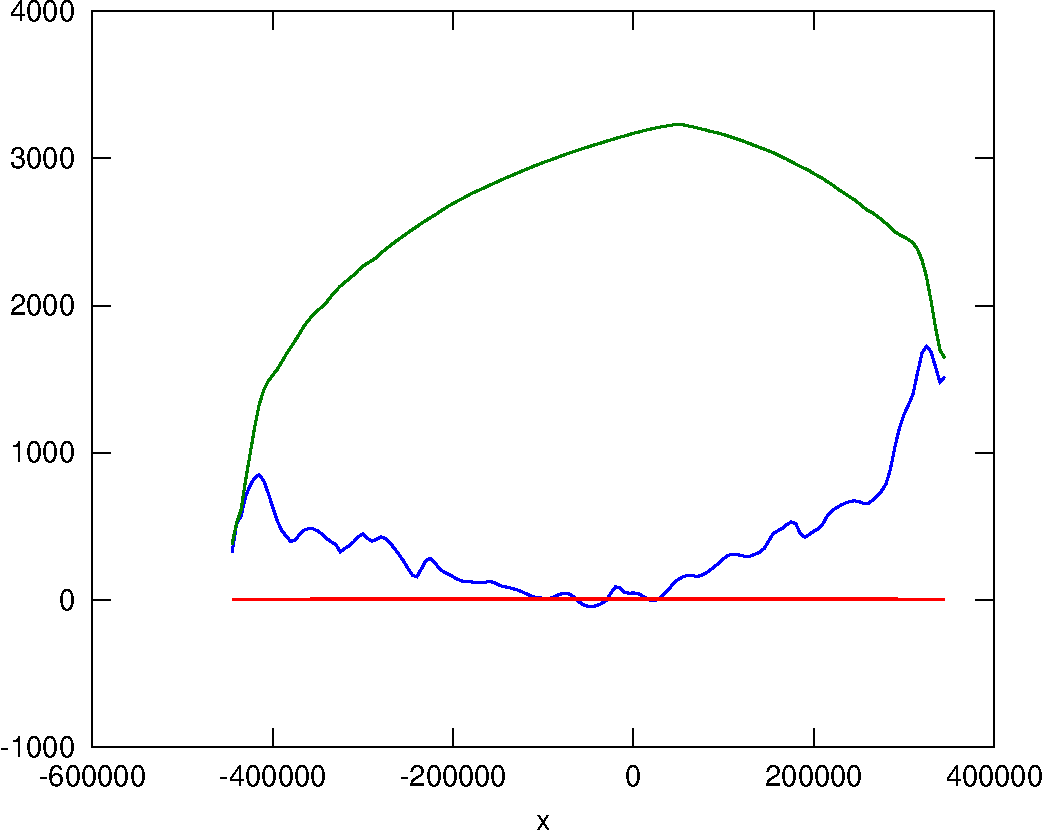
\includegraphics[width=0.4\textwidth]{green_transect} \\
%%       \footnotesize{Figure by E. Bueler}
%%     \end{center}
%%   \end{block}
%% \end{frame}

%% \begin{frame}{2. High Performance Computing (HPC)}
%%   \begin{block}{Exploit modern HPC through parallelism}
%%     \begin{figure}
%%       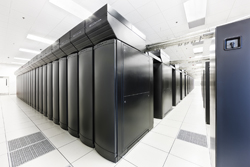
\includegraphics[width=5.5cm]{bw_front_sm}
%%       \hfill
%%       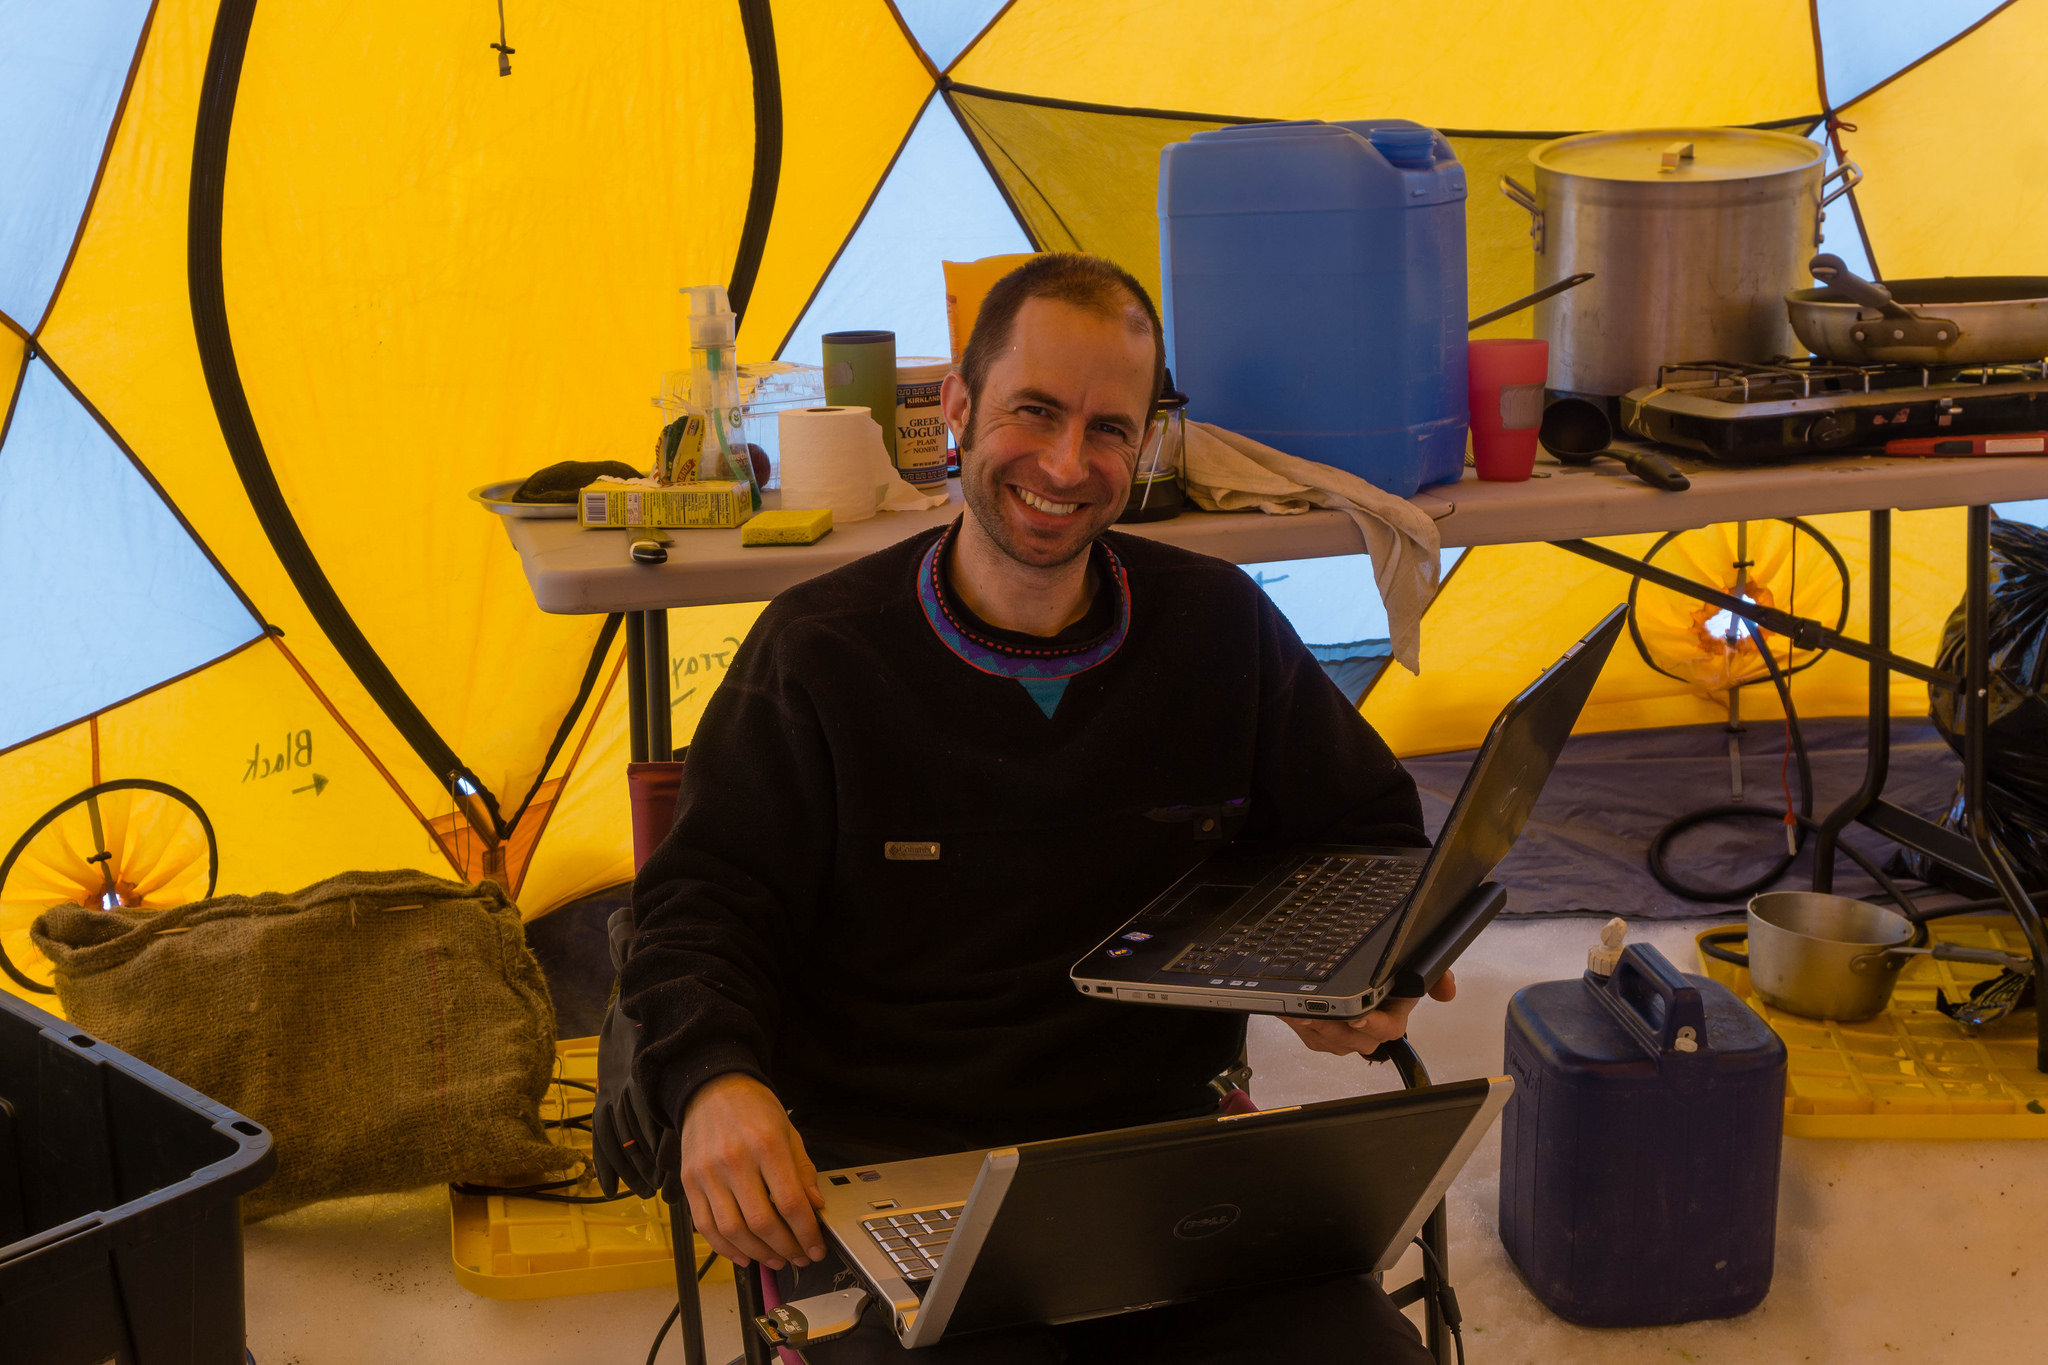
\includegraphics[width=5.5cm]{jason-parallel}
%%     \end{figure}
%%   \end{block}
%% \end{frame}

%% \begin{frame}{Challenge: ice thickness}
%%   \begin{columns}
%%     \column[c]{1.25cm}
%%     
\includegraphics[width=\textwidth]{nasa-logo} \\
%%     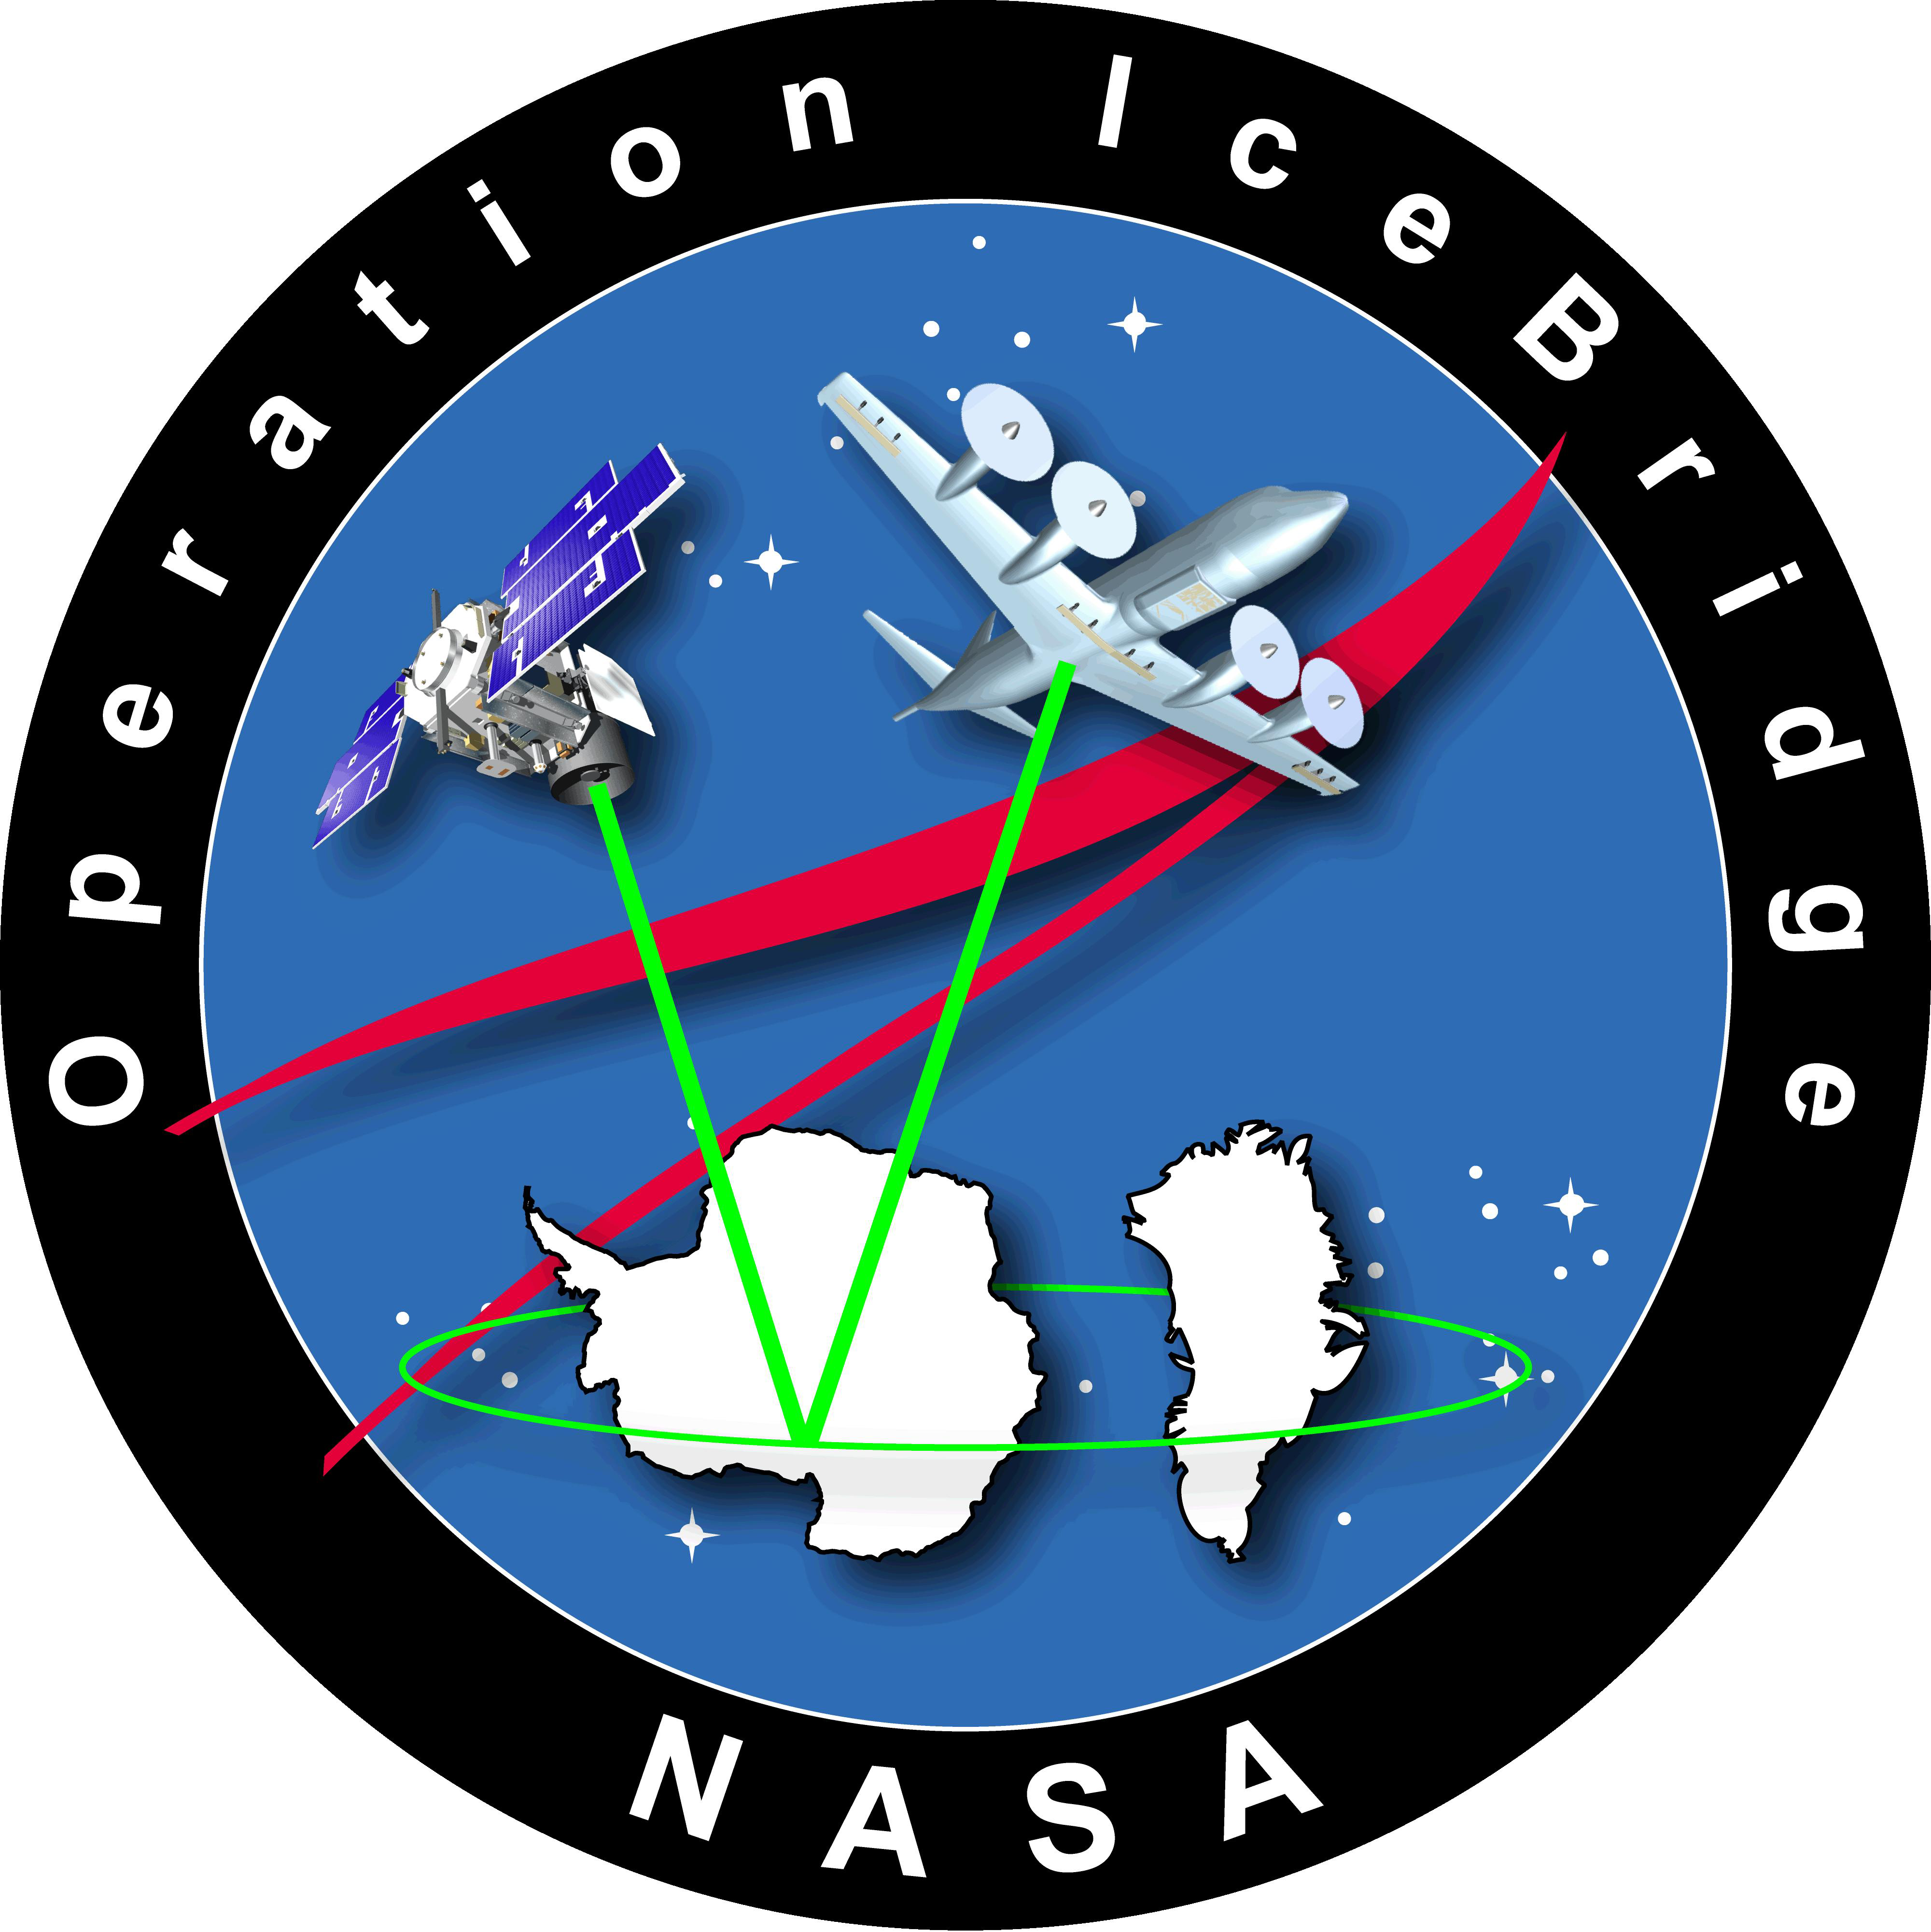
\includegraphics[width=\textwidth]{oib}
%%     \column[c]{10cm}
%%     \begin{itemize}
%%     \item ice thickness is a leading order constraint on ice flow
%%     \item but expensive to measure
%%     \item NASA realized that collecting a lot more ice thickness measurements is crucial to make ice sheet models better
%%     \item ice thickness measurements using the CReSIS radar became an important part of their Operation IceBridge mission (2009--2019)
%%     \end{itemize}
%%   \end{columns}
%%   \begin{figure}
%%     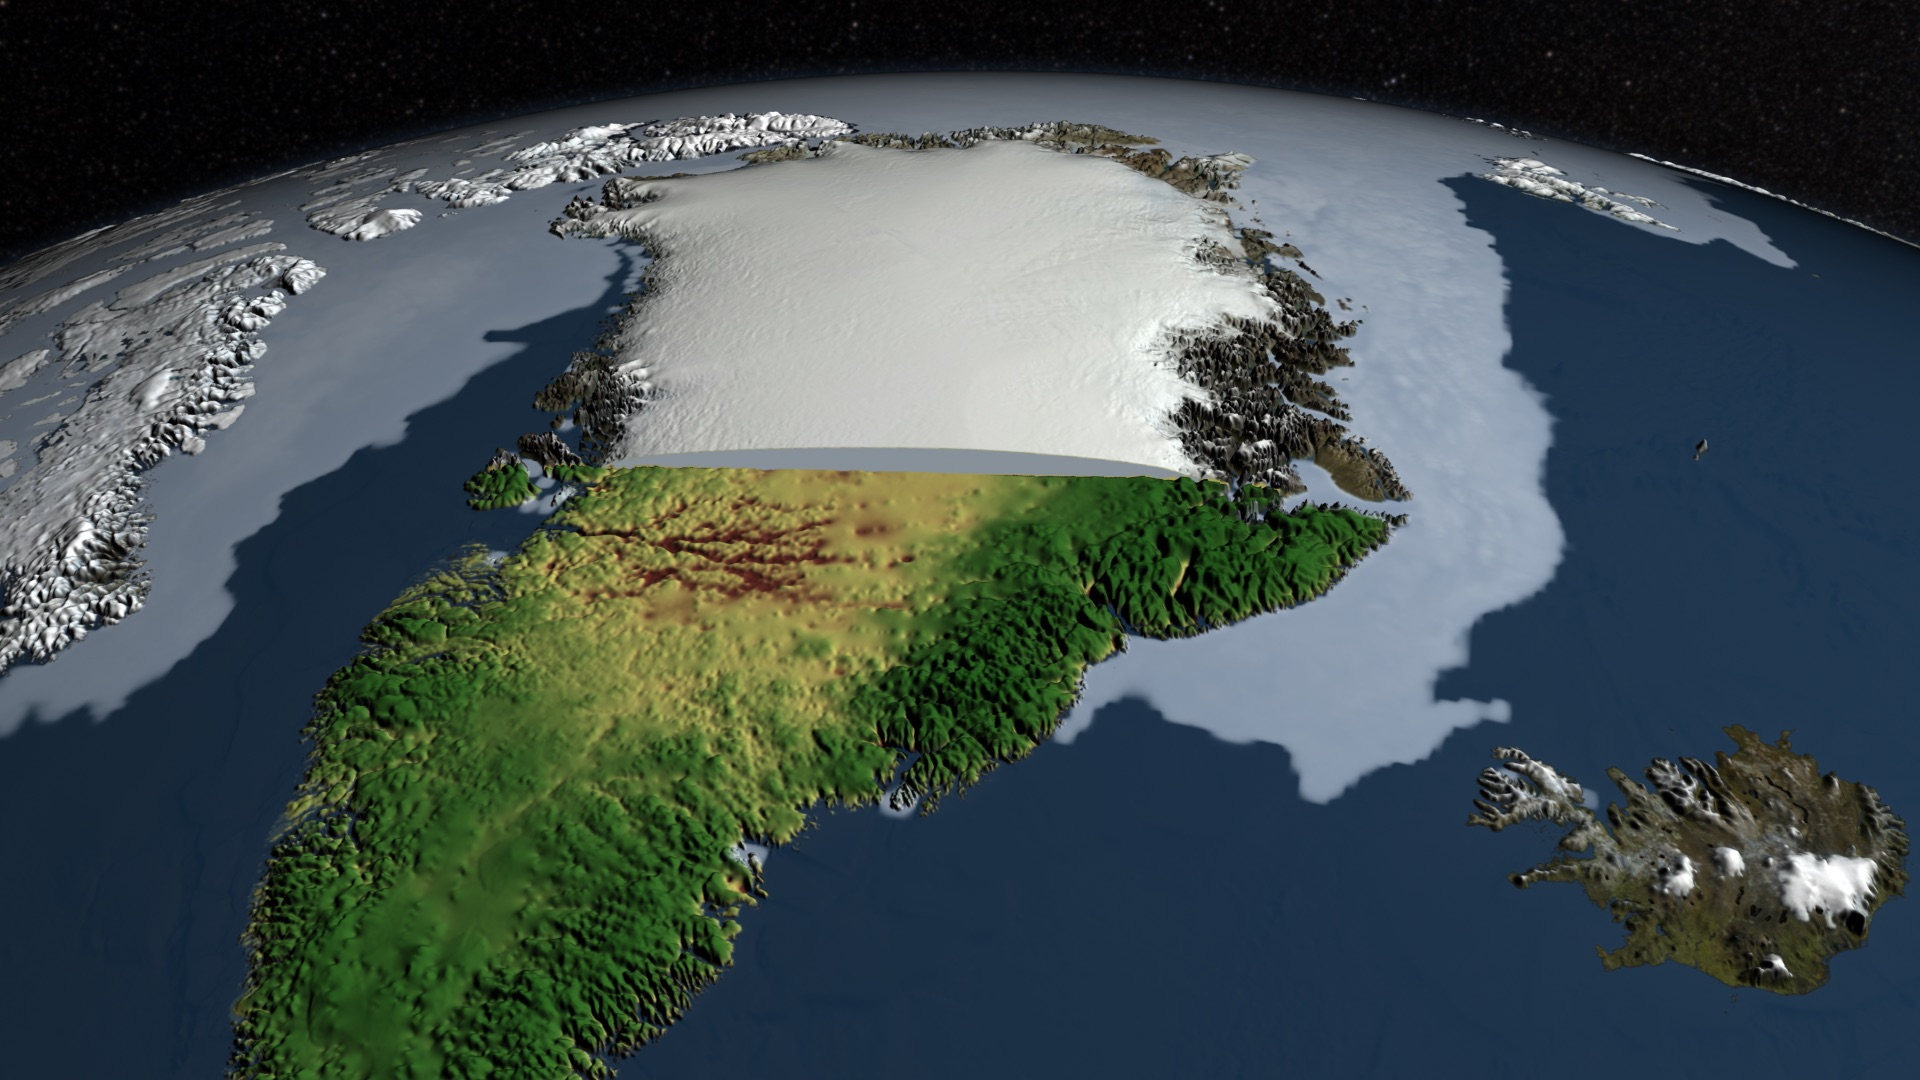
\includegraphics[width=6cm]{canale_grande_V05}
%%   \end{figure}
%% \note[item]{ice thickness is the difference between ice upper surface and the subglacial topography}
%% \end{frame}


%% \begin{frame}{NASA Operation IceBridge}
%%   \vspace{-0.74em}
%%   \begin{columns}
%%     \column[c]{4cm}
%%     \begin{itemize}
%%     \item additional flight lines since 2009
%%     \end{itemize}
%%     \column[c]{6cm}
%%     \begin{figure}
%%       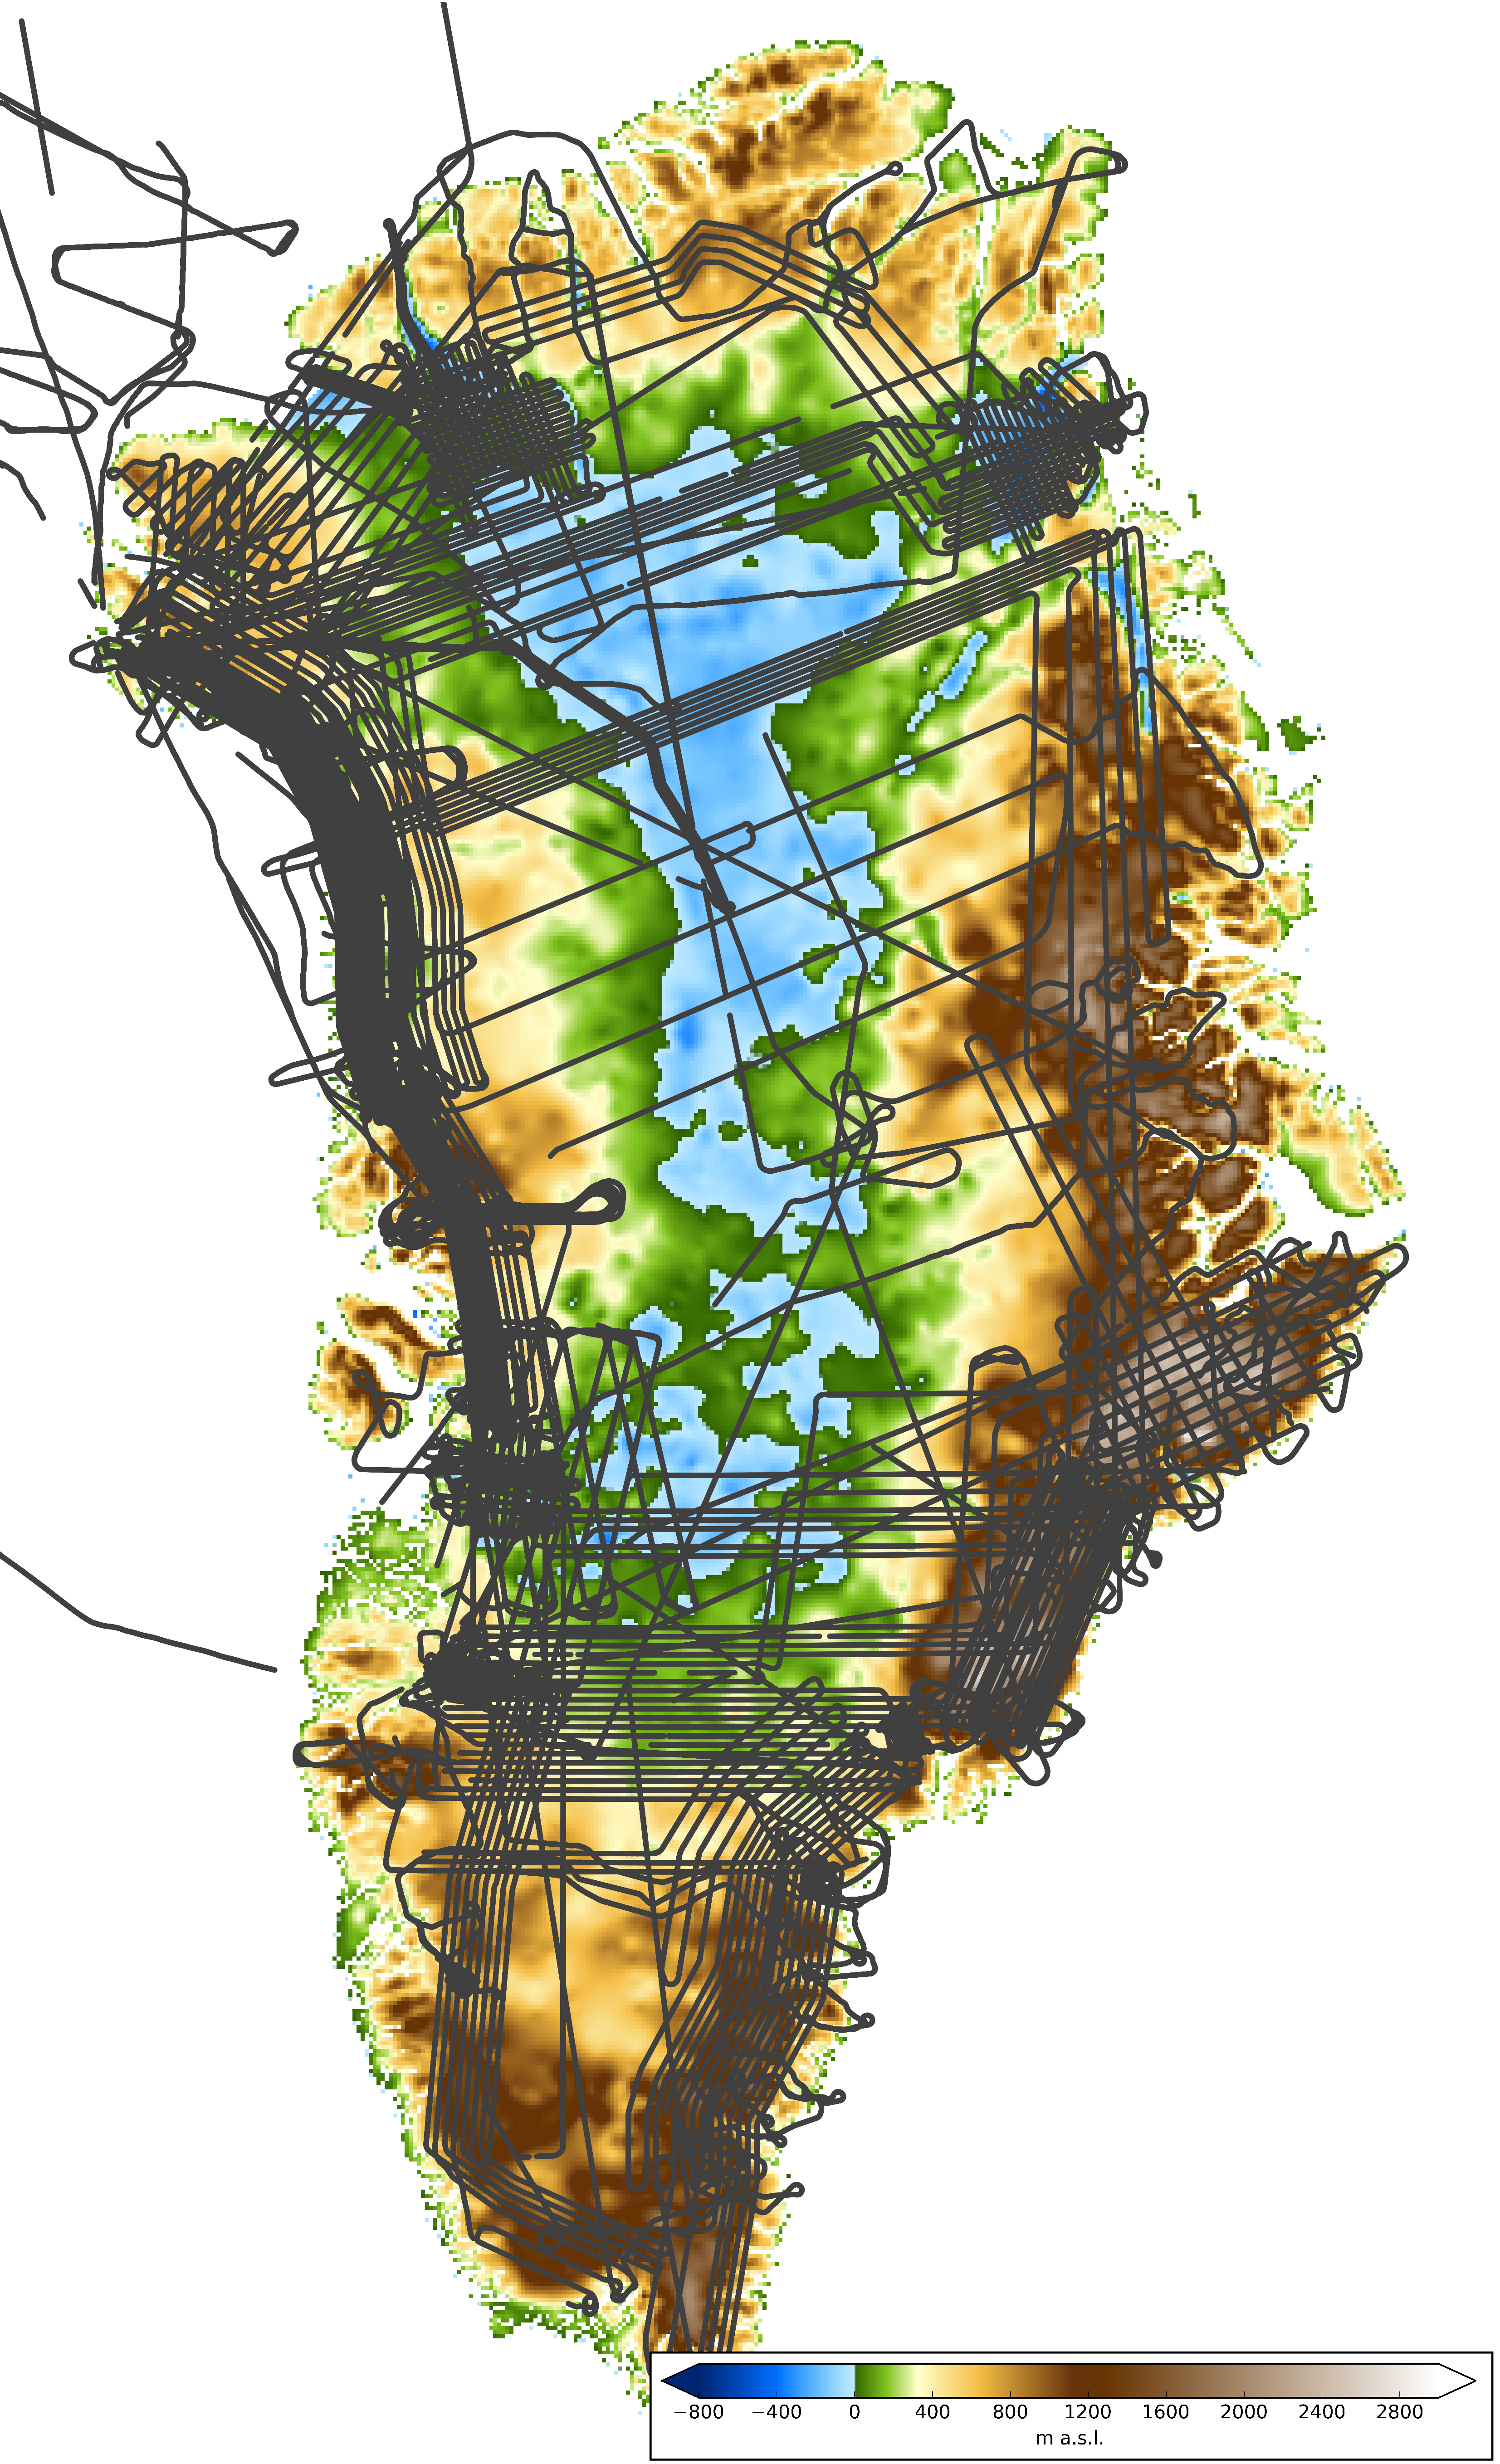
\includegraphics[height=8cm]{greenland-bed-old-oib}
%%     \end{figure}
%%   \end{columns}
%% \end{frame}

%% \begin{frame}{Zoom in to Jakobshavn Isbr{\ae}}
%%   \begin{figure}
%%     \small{old (2001) \hspace{5em} new (2014)}
%%     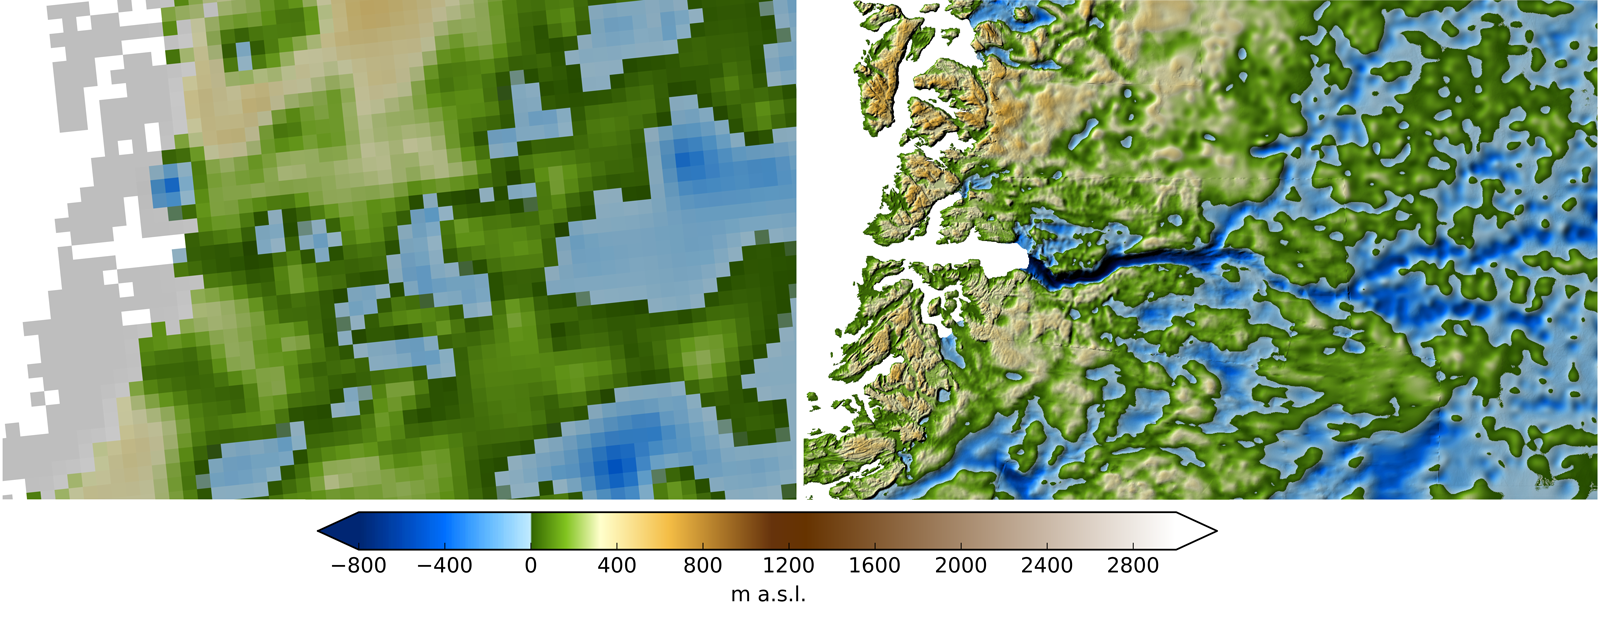
\includegraphics[width=12cm]{jako_bed}
%%  \end{figure}
%% \end{frame}


%% \begin{frame}{NASA Operation IceBridge}
%%   \begin{columns}
%%     \column[c]{8cm}
%%     \begin{figure}
%%       \small{old (2001) \hspace{4em} new (2014)}
%%       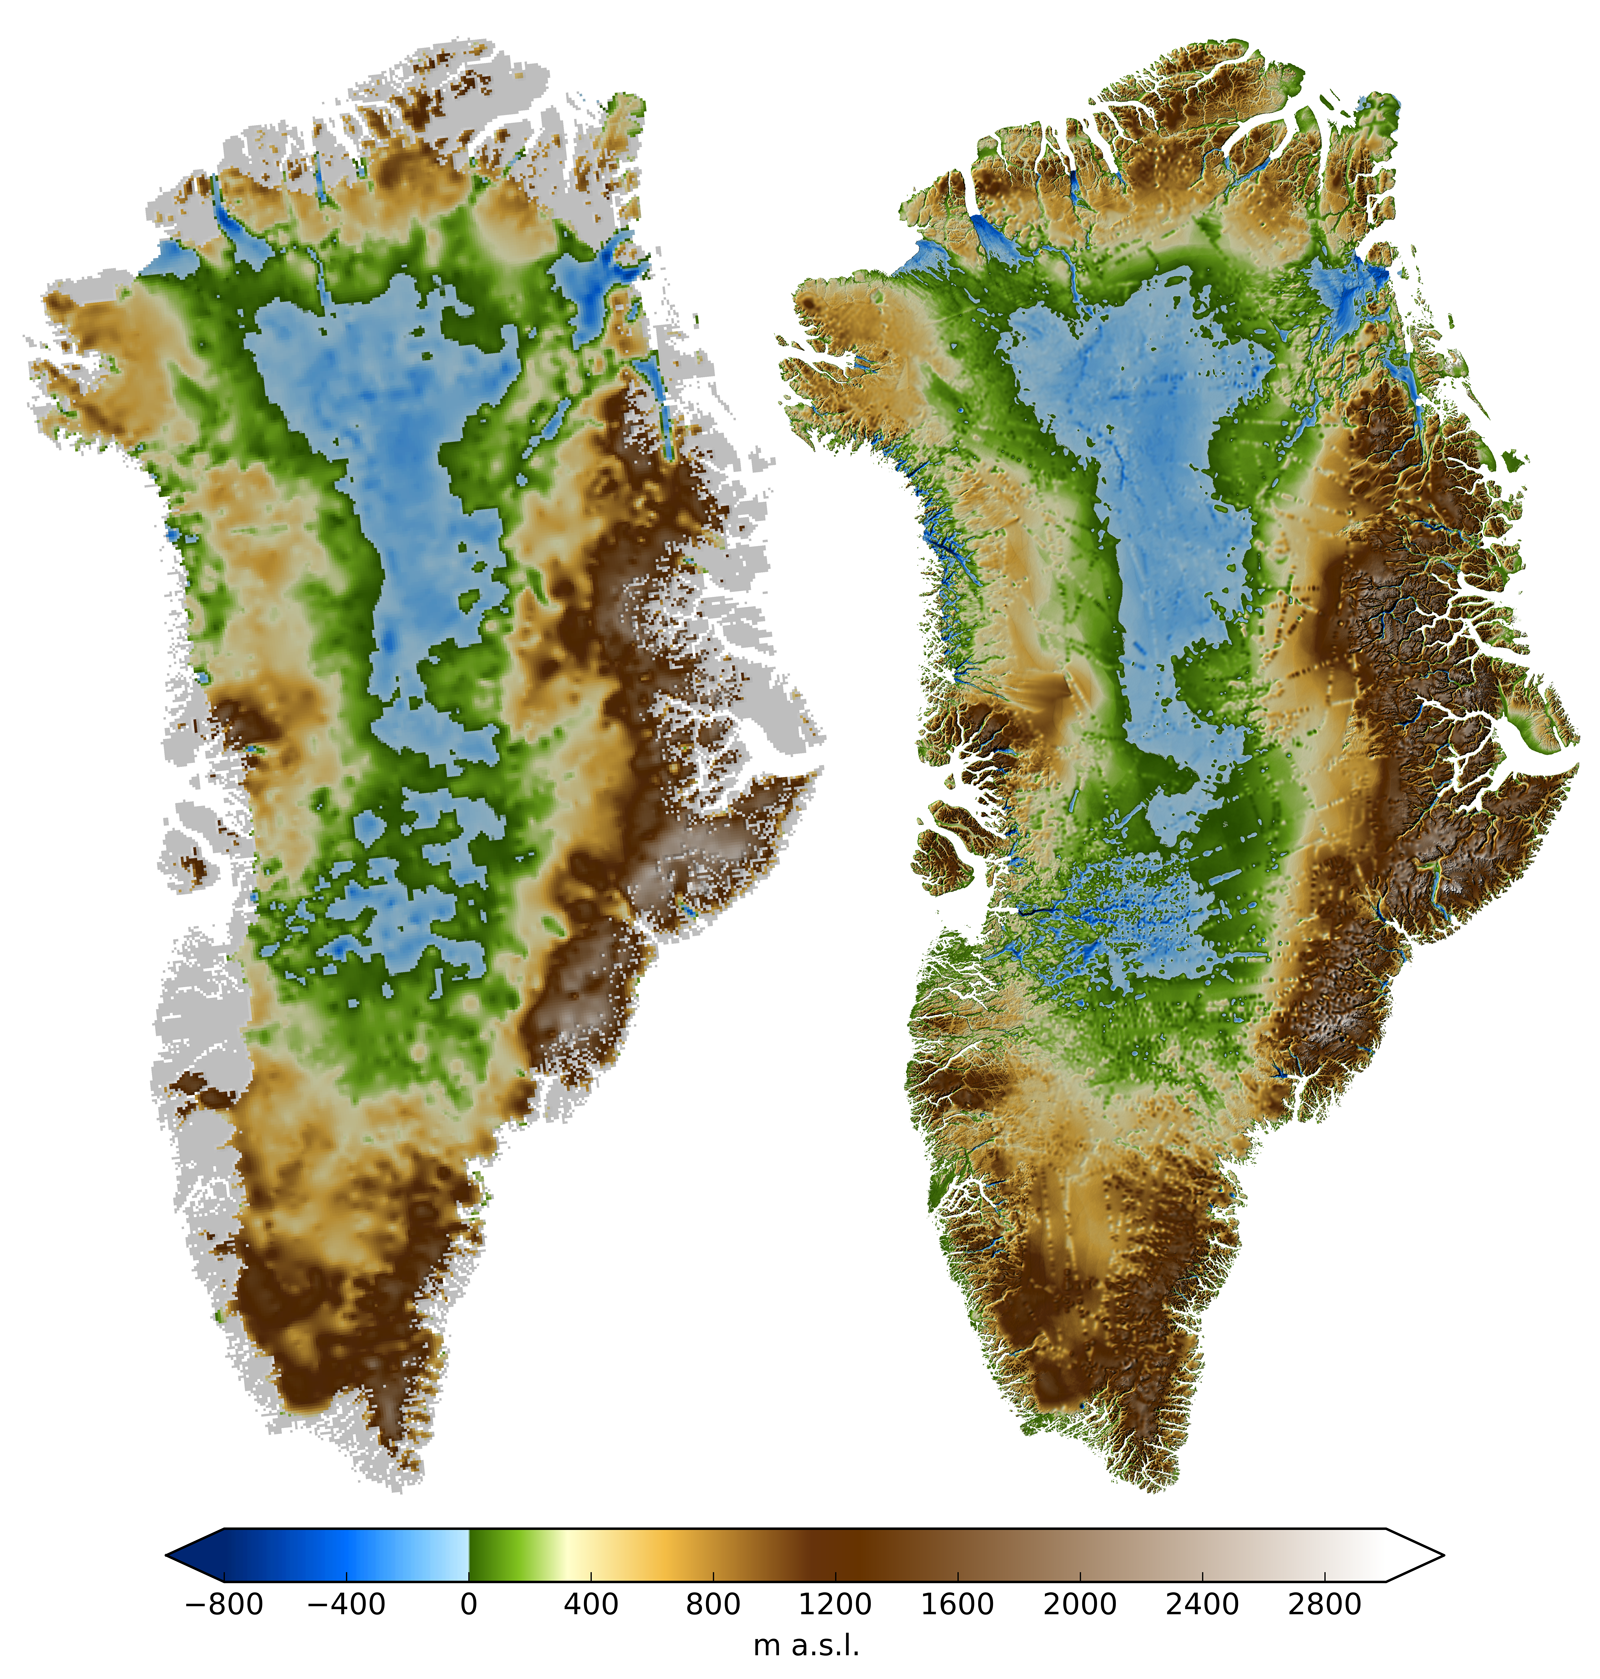
\includegraphics[height=7.5cm]{greenland_bed}
%%     \end{figure}
%%     \column[c]{4cm}
%%     \begin{itemize}
%%     \item from 5\,km to 150\,m horizontal grid resolution
%%     \end{itemize}
%%   \end{columns}
%% \end{frame}

%% \begin{frame}{NASA Operation IceBridge}
%%   \begin{figure}
%%     
\includegraphics[height=2.5cm]{nasa-logo} \qquad
%%     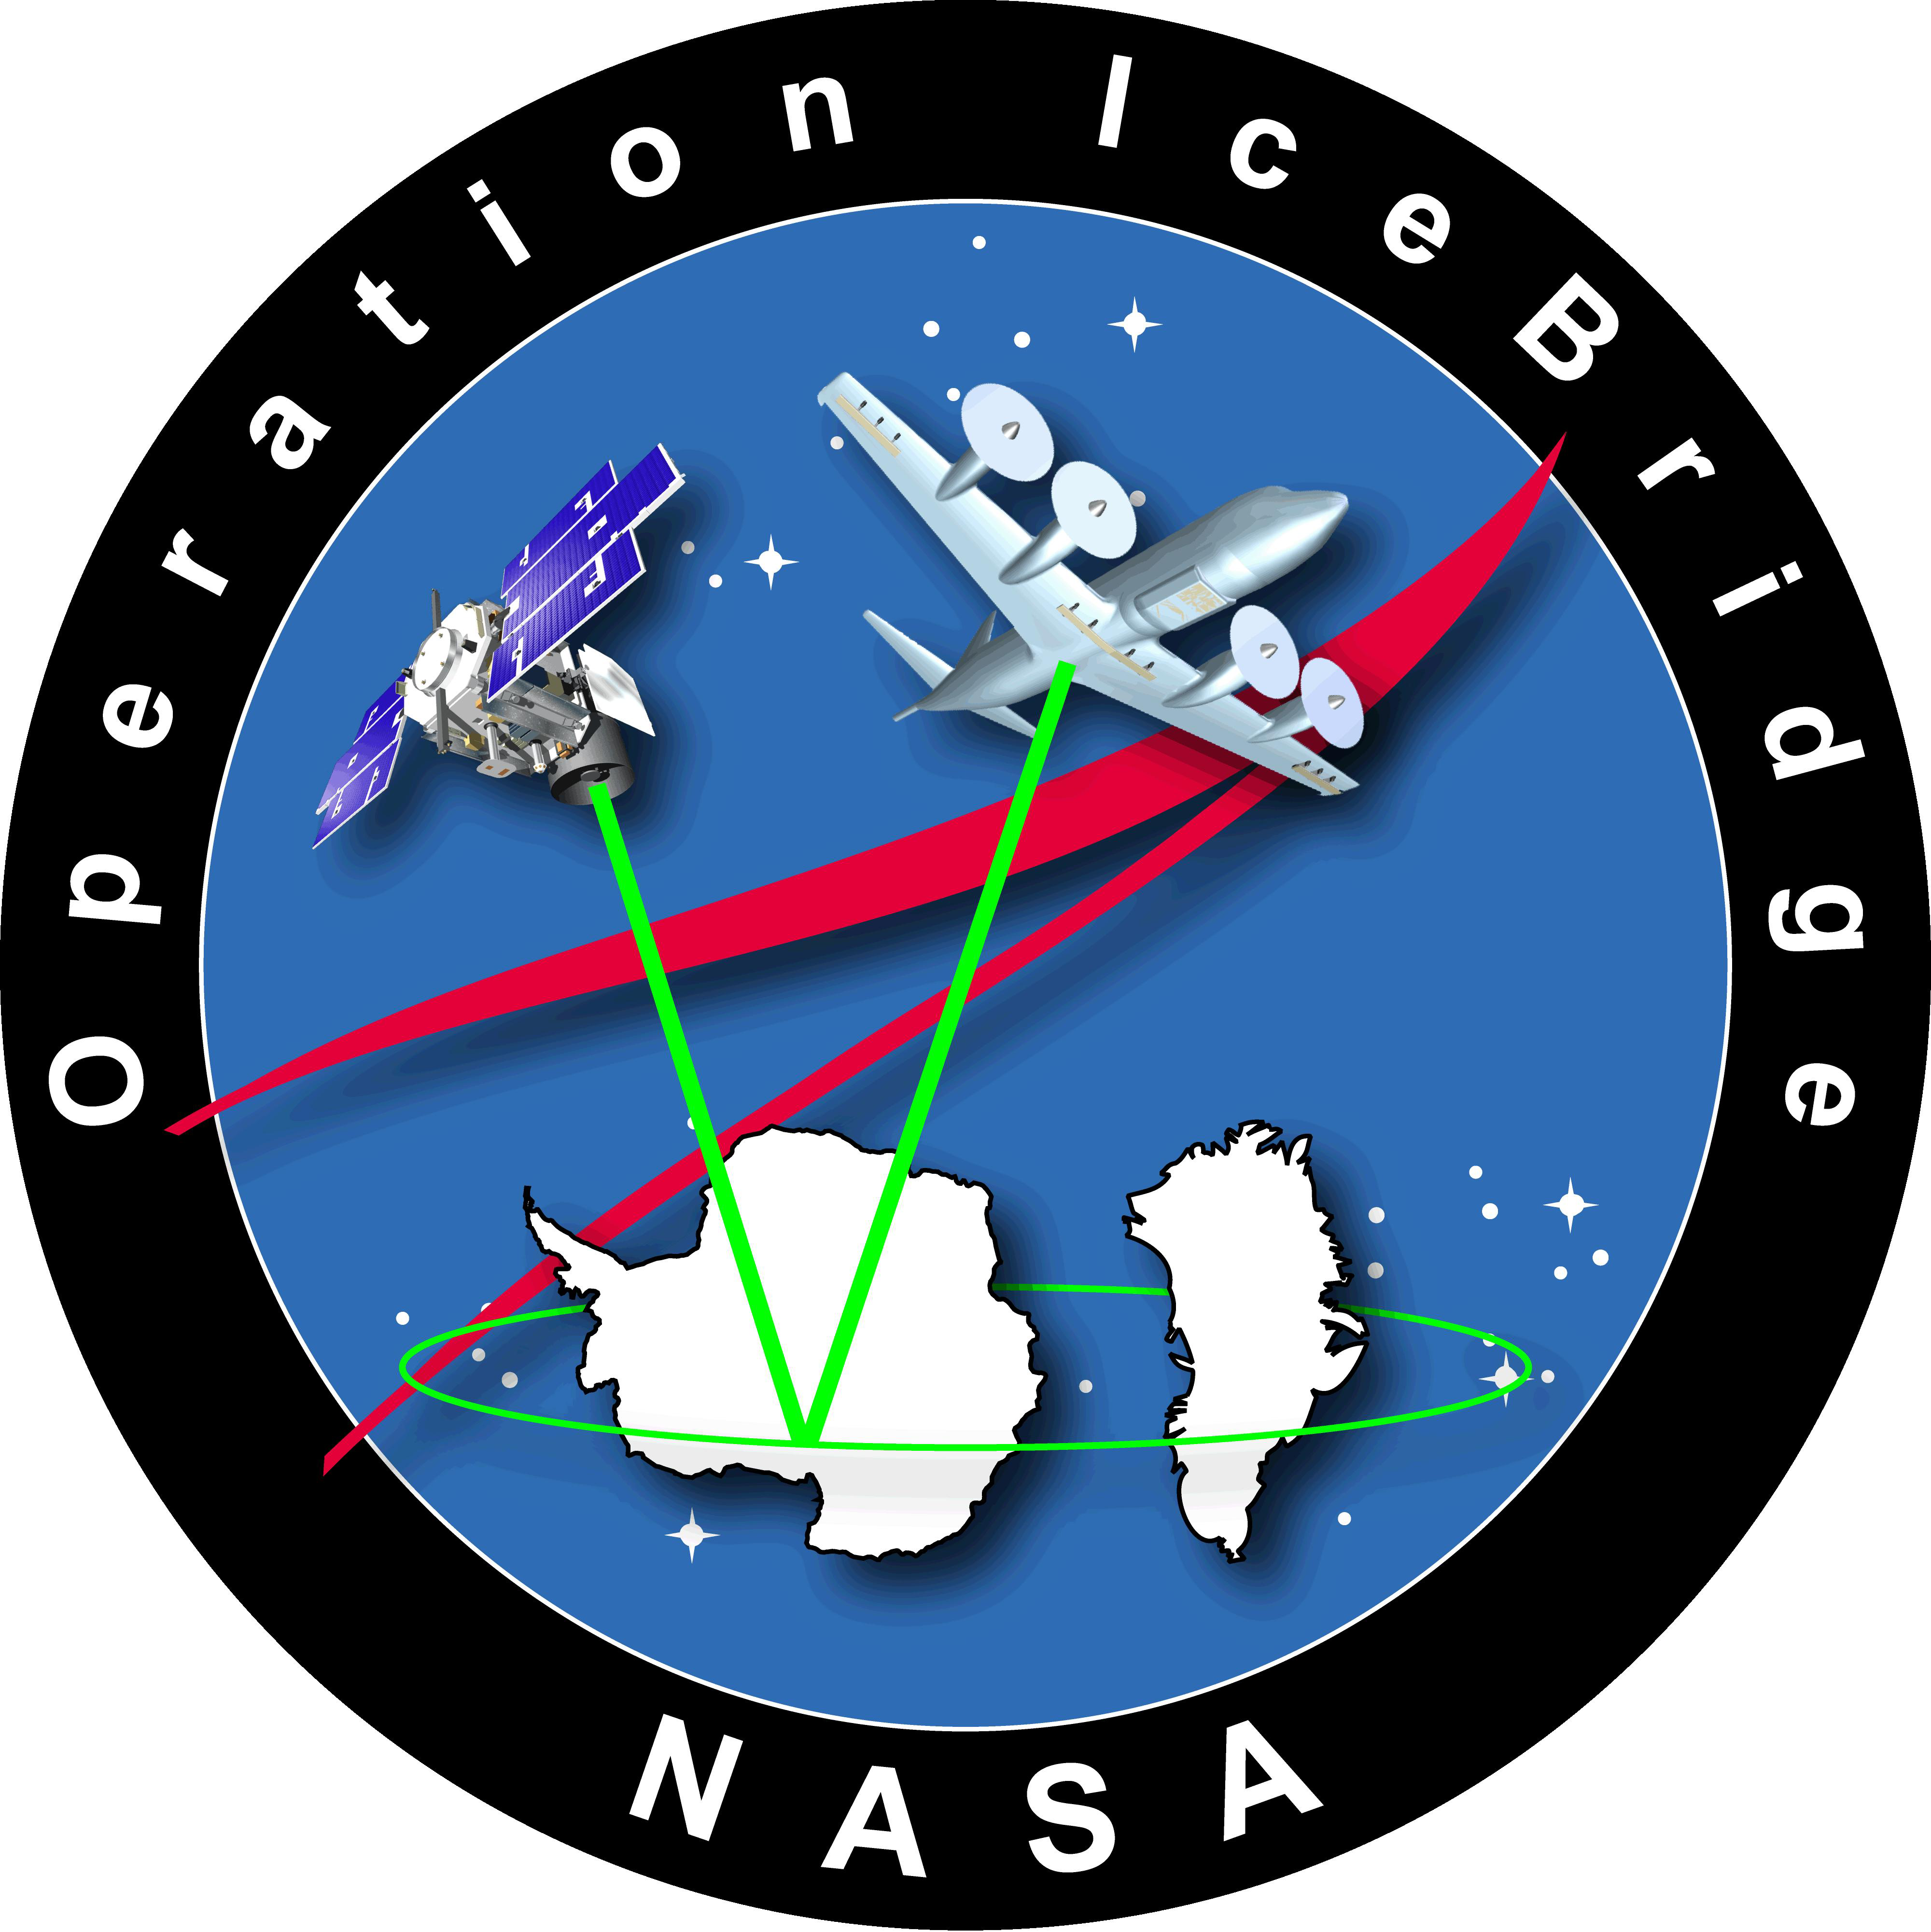
\includegraphics[height=2.5cm]{oib} \qquad
%%     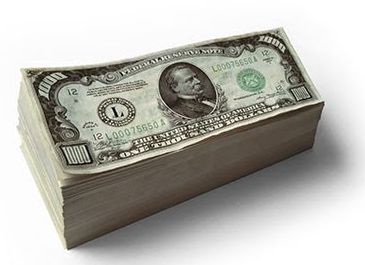
\includegraphics[height=2.5cm]{1000-dollar-bills}
%%   \end{figure}
%%   \begin{itemize}
%%   \item do NASA's OIB million\$ really make ice sheet models better?
%%   \end{itemize}
%%   \note[item]{so the multi million dollar question is}
%%   \note[item]{does this investment pay off?}
%% \end{frame}


%% \begin{frame}{Observed flow speeds}
%% \vspace{-0.74em}
%%   \begin{columns}
%%     \column[c]{5cm}
%%     \begin{figure}
%%       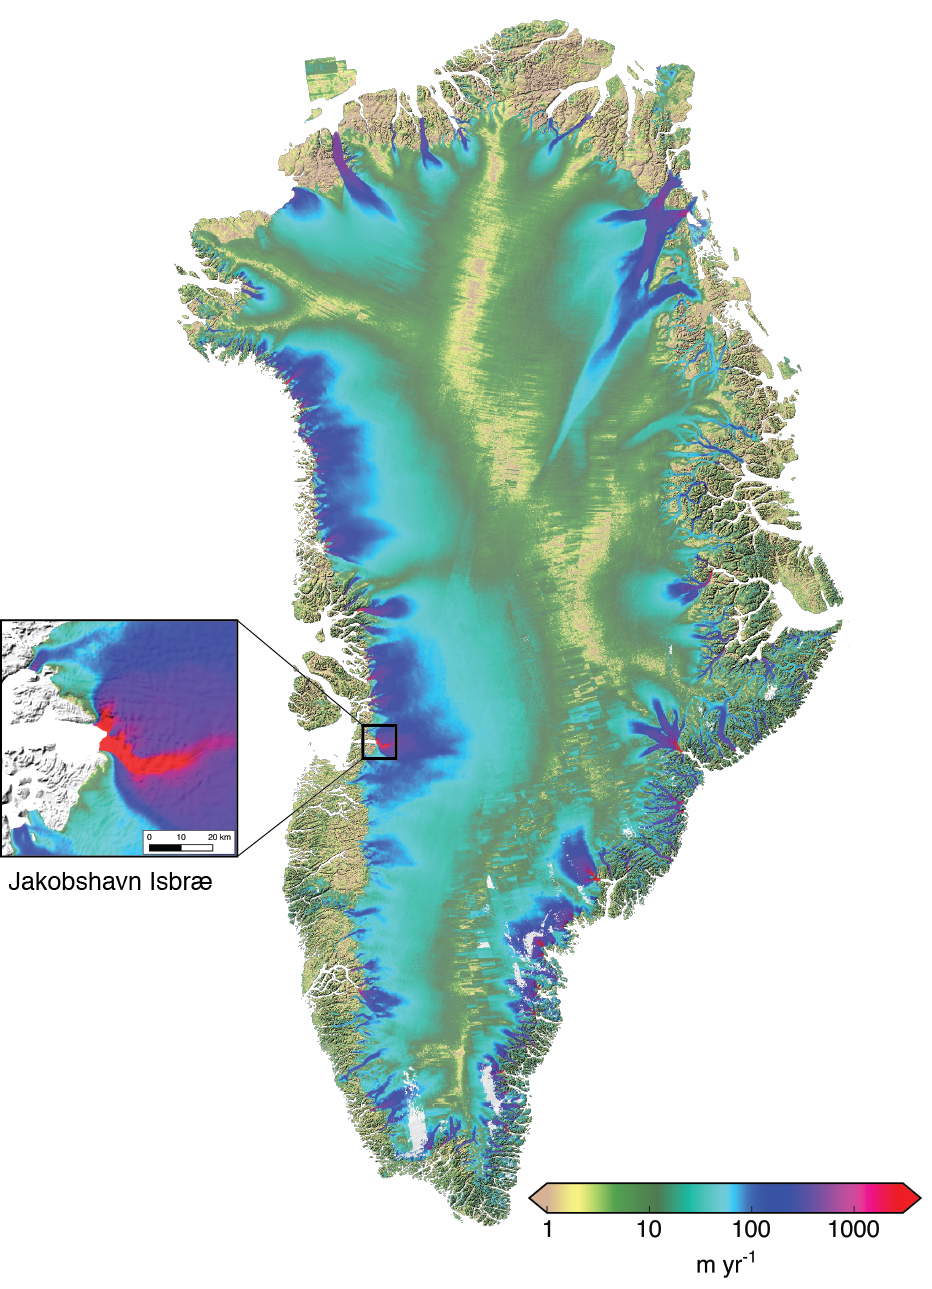
\includegraphics[width=\textwidth]{greenland-obs-overview}
%%     \end{figure}
%%     \column[c]{5cm}
%%     \only<1>{Jakobshavn Isbr{\ae}}
%%     \includegraphics<1>[width=\textwidth]{jakobshavn-obs-nogate}
%%     \only<1>{\\ {} }
%%   \end{columns}
%%   \note[item]{let's look at JIB again}
%%   \note[item]{observations show strongly channelized flow}
%%   \note[item]{with high flow speeds in the center}
%% \end{frame}


%% \begin{frame}{Ice thickness and simulated flow speeds}
%% \vspace{-0.74em}
%%   \begin{columns}
%%     \column[c]{5cm}
%%     \begin{figure}
%%       \includegraphics<1-2>[width=\textwidth]{greenland-obs-basal-overview}%
%%       \includegraphics<3-4>[width=\textwidth]{greenland-obs-basal-overview-mo14}%
%%     \end{figure}
%%     \column[c]{5cm}
%%     \only<1,3>{Jakobshavn Isbr{\ae}}
%%     \only<2>{no fast flow}
%%     \only<4>{fast flow appears}
%%     \includegraphics<1>[width=\textwidth]{jakobshavn-bed-5000m-ba01}%
%%     \includegraphics<2>[width=\textwidth]{jakobshavn-speed-exp-4500m-ba01}%
%%     \includegraphics<3>[width=\textwidth]{jakobshavn-bed-mo14}%
%%     \includegraphics<4>[width=\textwidth]{jakobshavn-speed-exp-600-v1.2-no-scale-no-gate}%
%%     \only<1>{\\ 5\,km, old data set (2001)}
%%     \only<2,4>{\\ simulated surface speed}
%%     \only<3>{\\ 600\,m, new data set (2014)}
%%   \end{columns}
%%   \note<1>[item]{now let's do a simualulation with the old ice thickness data}
%%   \note<2>[item]{there isn't really any fast flow}
%%   \note<3>[item]{now use the new ice thickness}
%%   \note<4>[item]{and we get fast flow}
%% \end{frame}


%% \begin{frame}{Can we capture the present-day flow field?}
%%   \begin{figure}
%%     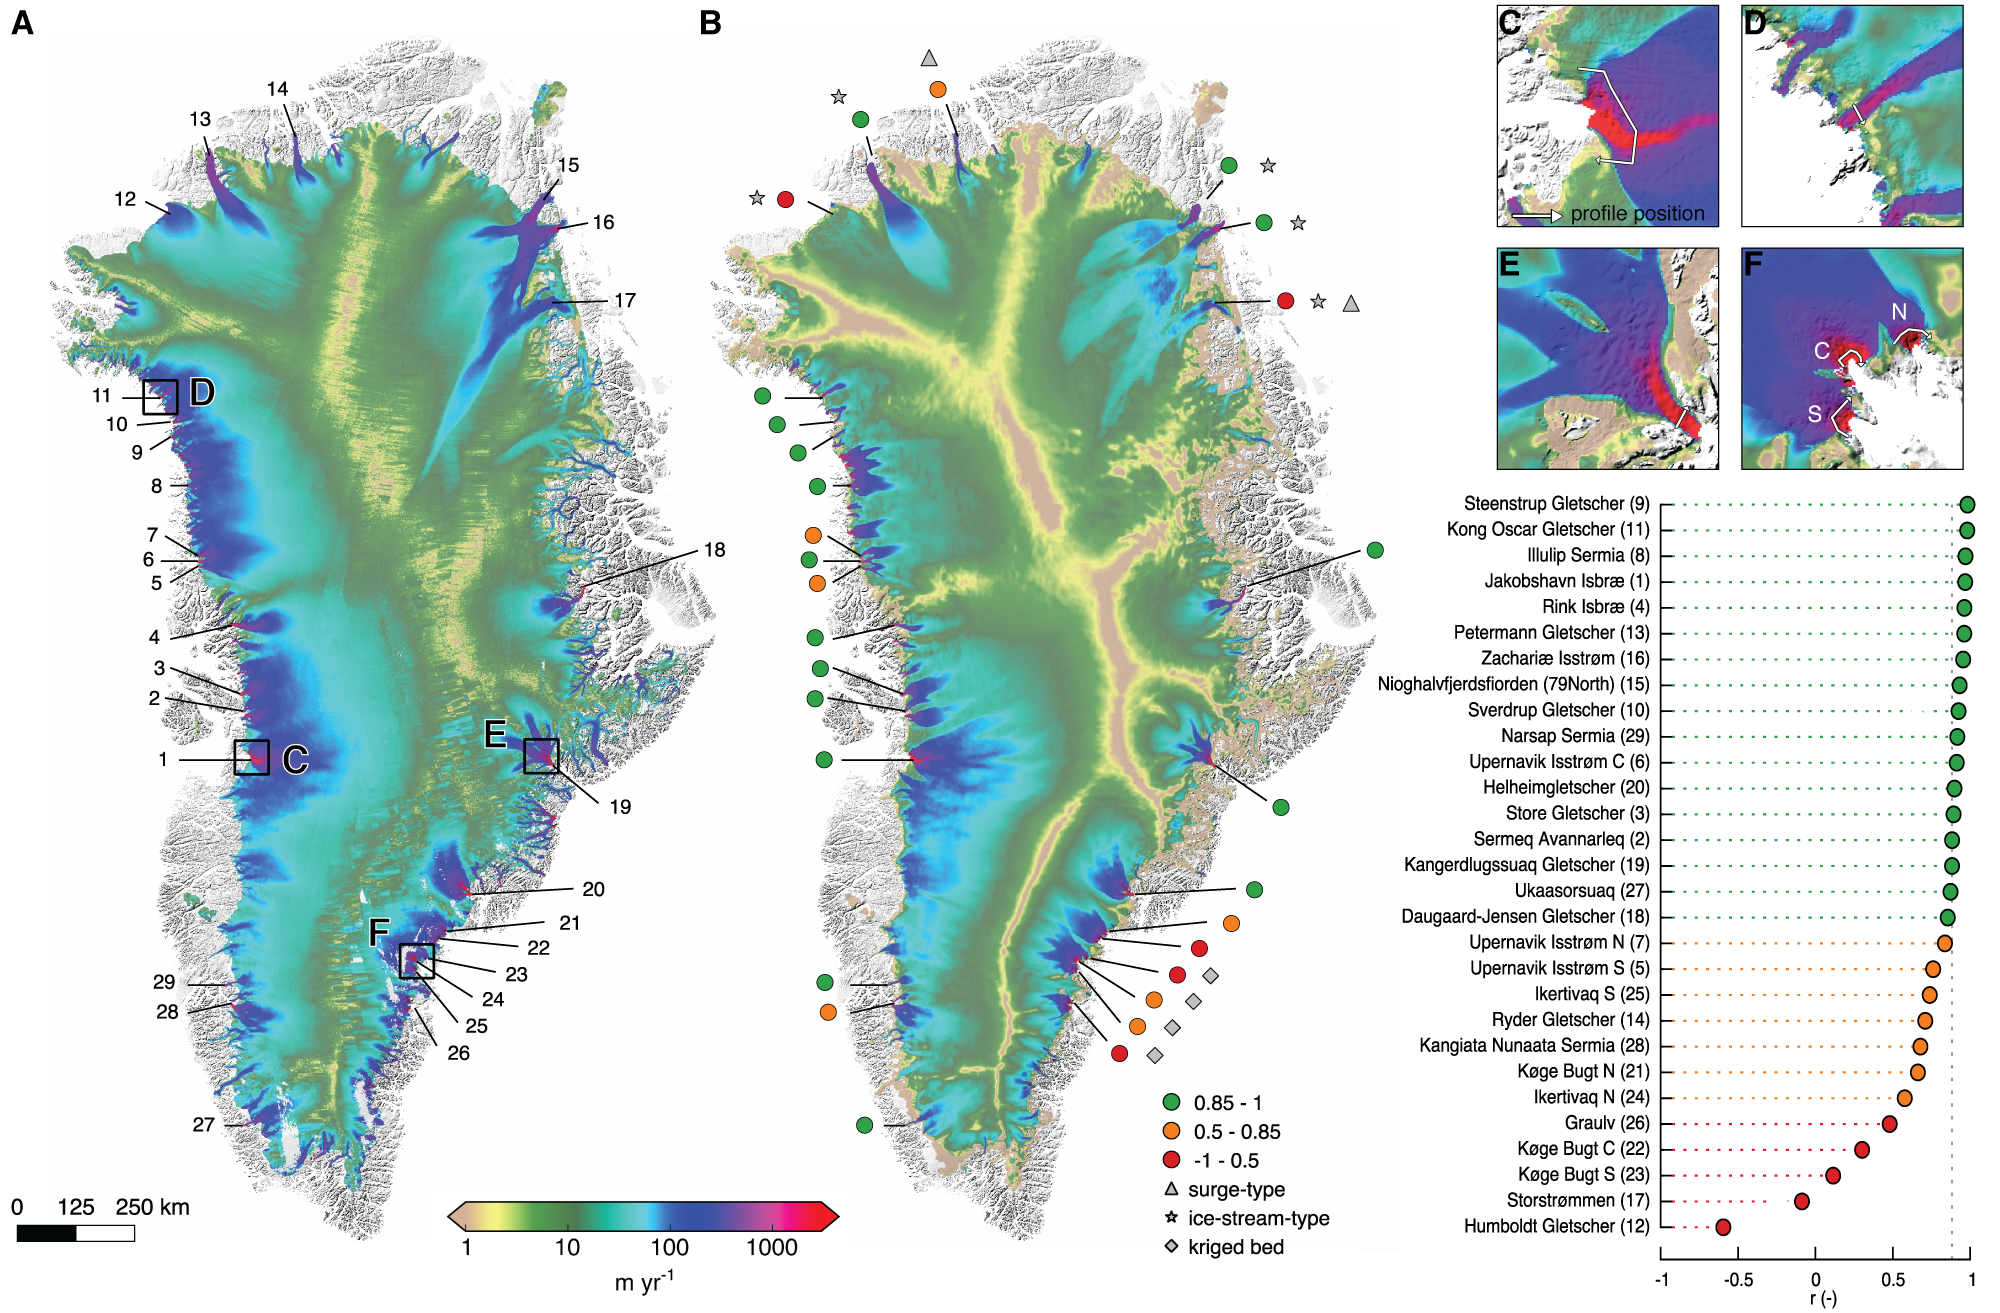
\includegraphics[height=7cm]{greenland-overview-3}
%%   \end{figure}
%%   \note[item]{first time capturing the flow field for the right reason}
%%   \note[item]{this is quite a break through in ice sheet modeling}
%%   \note[item]{though not a surprising one}
%%   \note[item]{it just confirms what students learn in glaciology 100:}
%%   \note[item]{ice flows downhill}
%% \end{frame}

\end{document}
